\documentclass[twoside]{book}

% Packages required by doxygen
\usepackage{fixltx2e}
\usepackage{calc}
\usepackage{doxygen}
\usepackage[export]{adjustbox} % also loads graphicx
\usepackage{graphicx}
\usepackage[utf8]{inputenc}
\usepackage{makeidx}
\usepackage{multicol}
\usepackage{multirow}
\PassOptionsToPackage{warn}{textcomp}
\usepackage{textcomp}
\usepackage[nointegrals]{wasysym}
\usepackage[table]{xcolor}

% Font selection
\usepackage[T1]{fontenc}
\usepackage[scaled=.90]{helvet}
\usepackage{courier}
\usepackage{amssymb}
\usepackage{sectsty}
\renewcommand{\familydefault}{\sfdefault}
\allsectionsfont{%
  \fontseries{bc}\selectfont%
  \color{darkgray}%
}
\renewcommand{\DoxyLabelFont}{%
  \fontseries{bc}\selectfont%
  \color{darkgray}%
}
\newcommand{\+}{\discretionary{\mbox{\scriptsize$\hookleftarrow$}}{}{}}

% Page & text layout
\usepackage{geometry}
\geometry{%
  a4paper,%
  top=2.5cm,%
  bottom=2.5cm,%
  left=2.5cm,%
  right=2.5cm%
}
\tolerance=750
\hfuzz=15pt
\hbadness=750
\setlength{\emergencystretch}{15pt}
\setlength{\parindent}{0cm}
\setlength{\parskip}{3ex plus 2ex minus 2ex}
\makeatletter
\renewcommand{\paragraph}{%
  \@startsection{paragraph}{4}{0ex}{-1.0ex}{1.0ex}{%
    \normalfont\normalsize\bfseries\SS@parafont%
  }%
}
\renewcommand{\subparagraph}{%
  \@startsection{subparagraph}{5}{0ex}{-1.0ex}{1.0ex}{%
    \normalfont\normalsize\bfseries\SS@subparafont%
  }%
}
\makeatother

% Headers & footers
\usepackage{fancyhdr}
\pagestyle{fancyplain}
\fancyhead[LE]{\fancyplain{}{\bfseries\thepage}}
\fancyhead[CE]{\fancyplain{}{}}
\fancyhead[RE]{\fancyplain{}{\bfseries\leftmark}}
\fancyhead[LO]{\fancyplain{}{\bfseries\rightmark}}
\fancyhead[CO]{\fancyplain{}{}}
\fancyhead[RO]{\fancyplain{}{\bfseries\thepage}}
\fancyfoot[LE]{\fancyplain{}{}}
\fancyfoot[CE]{\fancyplain{}{}}
\fancyfoot[RE]{\fancyplain{}{\bfseries\scriptsize Gandhi Games }}
\fancyfoot[LO]{\fancyplain{}{\bfseries\scriptsize Fractal Trees With Springs }}
\fancyfoot[CO]{\fancyplain{}{}}
\fancyfoot[RO]{\fancyplain{}{}}
\renewcommand{\footrulewidth}{0.4pt}
\renewcommand{\chaptermark}[1]{%
  \markboth{#1}{}%
}
\renewcommand{\sectionmark}[1]{%
  \markright{\thesection\ #1}%
}

% Indices & bibliography
\usepackage{natbib}
\usepackage[titles]{tocloft}
\setcounter{tocdepth}{3}
\setcounter{secnumdepth}{5}
\makeindex

% Hyperlinks (required, but should be loaded last)
\usepackage{ifpdf}
\ifpdf
  \usepackage[pdftex,pagebackref=true]{hyperref}
\else
  \usepackage[ps2pdf,pagebackref=true]{hyperref}
\fi
\hypersetup{%
  colorlinks=true,%
  linkcolor=blue,%
  citecolor=blue,%
  unicode%
}

% Custom commands
\newcommand{\clearemptydoublepage}{%
  \newpage{\pagestyle{empty}\cleardoublepage}%
}

\usepackage{caption}
\captionsetup{labelsep=space,justification=centering,font={bf},singlelinecheck=off,skip=4pt,position=top}

%===== C O N T E N T S =====

\begin{document}

% Titlepage & ToC
\hypersetup{pageanchor=false,
             bookmarksnumbered=true,
             pdfencoding=unicode
            }
\pagenumbering{alph}
\begin{titlepage}
\vspace*{7cm}
\begin{center}%
{\Large Fractal Trees With Springs \\[1ex]\large 0.\+1 }\\
\vspace*{1cm}
{\large Gandhi Games}\\
\end{center}
\end{titlepage}
\clearemptydoublepage
\pagenumbering{roman}
\tableofcontents
\clearemptydoublepage
\pagenumbering{arabic}
\hypersetup{pageanchor=true}

%--- Begin generated contents ---
\chapter{Namespace Index}
\section{Packages}
Here are the packages with brief descriptions (if available)\+:\begin{DoxyCompactList}
\item\contentsline{section}{\hyperlink{namespace_fractal_tree}{Fractal\+Tree} }{\pageref{namespace_fractal_tree}}{}
\end{DoxyCompactList}

\chapter{Hierarchical Index}
\section{Class Hierarchy}
This inheritance list is sorted roughly, but not completely, alphabetically\+:\begin{DoxyCompactList}
\item \contentsline{section}{Fractal\+Tree.\+Branch}{\pageref{interface_fractal_tree_1_1_branch}}{}
\begin{DoxyCompactList}
\item \contentsline{section}{Fractal\+Tree.\+Moving\+Branch}{\pageref{interface_fractal_tree_1_1_moving_branch}}{}
\begin{DoxyCompactList}
\item \contentsline{section}{Fractal\+Tree.\+Moving\+Branch\+Impl}{\pageref{class_fractal_tree_1_1_moving_branch_impl}}{}
\end{DoxyCompactList}
\item \contentsline{section}{Fractal\+Tree.\+Stationary\+Branch}{\pageref{class_fractal_tree_1_1_stationary_branch}}{}
\begin{DoxyCompactList}
\item \contentsline{section}{Fractal\+Tree.\+Moving\+Branch\+Impl}{\pageref{class_fractal_tree_1_1_moving_branch_impl}}{}
\end{DoxyCompactList}
\end{DoxyCompactList}
\item Editor\begin{DoxyCompactList}
\item \contentsline{section}{Fractal\+Tree.\+Tree\+Builder\+Editor}{\pageref{class_fractal_tree_1_1_tree_builder_editor}}{}
\begin{DoxyCompactList}
\item \contentsline{section}{Fractal\+Tree.\+Moving\+Tree\+Builder\+Editor}{\pageref{class_fractal_tree_1_1_moving_tree_builder_editor}}{}
\item \contentsline{section}{Fractal\+Tree.\+Stationary\+Tree\+Builder\+Editor}{\pageref{class_fractal_tree_1_1_stationary_tree_builder_editor}}{}
\end{DoxyCompactList}
\end{DoxyCompactList}
\item \contentsline{section}{Fractal\+Tree.\+L\+Rule}{\pageref{class_fractal_tree_1_1_l_rule}}{}
\item Mono\+Behaviour\begin{DoxyCompactList}
\item \contentsline{section}{Fractal\+Tree.\+Colonization\+Leaf}{\pageref{class_fractal_tree_1_1_colonization_leaf}}{}
\item \contentsline{section}{Fractal\+Tree.\+Colonization\+Leaf\+Generator}{\pageref{class_fractal_tree_1_1_colonization_leaf_generator}}{}
\item \contentsline{section}{Fractal\+Tree.\+Demo.\+Demo\+Branch\+Tree\+UI}{\pageref{class_fractal_tree_1_1_demo_1_1_demo_branch_tree_u_i}}{}
\item \contentsline{section}{Fractal\+Tree.\+Demo.\+Demo\+Colonization\+Tree\+UI}{\pageref{class_fractal_tree_1_1_demo_1_1_demo_colonization_tree_u_i}}{}
\item \contentsline{section}{Fractal\+Tree.\+Demo.\+Demo\+Controls}{\pageref{class_fractal_tree_1_1_demo_1_1_demo_controls}}{}
\item \contentsline{section}{Fractal\+Tree.\+Demo.\+Demo\+Force\+Controller}{\pageref{class_fractal_tree_1_1_demo_1_1_demo_force_controller}}{}
\item \contentsline{section}{Fractal\+Tree.\+Demo.\+Demo\+L\+Tree\+UI}{\pageref{class_fractal_tree_1_1_demo_1_1_demo_l_tree_u_i}}{}
\item \contentsline{section}{Fractal\+Tree.\+Demo.\+Demo\+Scene\+Switcher}{\pageref{class_fractal_tree_1_1_demo_1_1_demo_scene_switcher}}{}
\item \contentsline{section}{Fractal\+Tree.\+Demo.\+Demo\+Tree\+Creator}{\pageref{class_fractal_tree_1_1_demo_1_1_demo_tree_creator}}{}
\item \contentsline{section}{Fractal\+Tree.\+Demo.\+Demo\+Tree\+Data}{\pageref{class_fractal_tree_1_1_demo_1_1_demo_tree_data}}{}
\item \contentsline{section}{Fractal\+Tree.\+Demo\+Leaf\+Placement}{\pageref{class_fractal_tree_1_1_demo_leaf_placement}}{}
\item \contentsline{section}{Fractal\+Tree.\+Spring}{\pageref{class_fractal_tree_1_1_spring}}{}
\item \contentsline{section}{Fractal\+Tree.\+Stationary\+Branch}{\pageref{class_fractal_tree_1_1_stationary_branch}}{}
\item \contentsline{section}{Fractal\+Tree.\+Tree\+Builder}{\pageref{class_fractal_tree_1_1_tree_builder}}{}
\begin{DoxyCompactList}
\item \contentsline{section}{Fractal\+Tree.\+Moving\+Tree\+Builder}{\pageref{class_fractal_tree_1_1_moving_tree_builder}}{}
\item \contentsline{section}{Fractal\+Tree.\+Stationary\+Tree\+Builder}{\pageref{class_fractal_tree_1_1_stationary_tree_builder}}{}
\end{DoxyCompactList}
\end{DoxyCompactList}
\item \contentsline{section}{Fractal\+Tree.\+Point\+Mass}{\pageref{class_fractal_tree_1_1_point_mass}}{}
\item \contentsline{section}{Fractal\+Tree.\+Tree}{\pageref{interface_fractal_tree_1_1_tree}}{}
\begin{DoxyCompactList}
\item \contentsline{section}{Fractal\+Tree.\+Colonization\+Tree}{\pageref{class_fractal_tree_1_1_colonization_tree}}{}
\item \contentsline{section}{Fractal\+Tree.\+Default\+Tree}{\pageref{class_fractal_tree_1_1_default_tree}}{}
\item \contentsline{section}{Fractal\+Tree.\+L\+Tree}{\pageref{class_fractal_tree_1_1_l_tree}}{}
\end{DoxyCompactList}
\item \contentsline{section}{Fractal\+Tree.\+Demo.\+Trees\+To\+Demo}{\pageref{class_fractal_tree_1_1_demo_1_1_trees_to_demo}}{}
\end{DoxyCompactList}

\chapter{Class Index}
\section{Class List}
Here are the classes, structs, unions and interfaces with brief descriptions\+:\begin{DoxyCompactList}
\item\contentsline{section}{\hyperlink{interface_fractal_tree_1_1_branch}{Fractal\+Tree.\+Branch} \\*Contract for all fractal tree branches. Includes positional data and initialisation. }{\pageref{interface_fractal_tree_1_1_branch}}{}
\item\contentsline{section}{\hyperlink{class_fractal_tree_1_1_colonization_leaf}{Fractal\+Tree.\+Colonization\+Leaf} \\*Attach to leaf objects for space colonization. The branches move towards the leaves. }{\pageref{class_fractal_tree_1_1_colonization_leaf}}{}
\item\contentsline{section}{\hyperlink{class_fractal_tree_1_1_colonization_leaf_generator}{Fractal\+Tree.\+Colonization\+Leaf\+Generator} \\*Spawns a set number of leaves within a bounds. Used by space colonization. }{\pageref{class_fractal_tree_1_1_colonization_leaf_generator}}{}
\item\contentsline{section}{\hyperlink{class_fractal_tree_1_1_colonization_tree}{Fractal\+Tree.\+Colonization\+Tree} \\*Spawns a fractal tree using space colonization\+: \href{http://algorithmicbotany.org/papers/colonization.egwnp2007.pdf}{\tt http\+://algorithmicbotany.\+org/papers/colonization.\+egwnp2007.\+pdf} }{\pageref{class_fractal_tree_1_1_colonization_tree}}{}
\item\contentsline{section}{\hyperlink{class_fractal_tree_1_1_default_tree}{Fractal\+Tree.\+Default\+Tree} \\*Spawns a fractal tree. }{\pageref{class_fractal_tree_1_1_default_tree}}{}
\item\contentsline{section}{\hyperlink{class_fractal_tree_1_1_demo_1_1_demo_branch_tree_u_i}{Fractal\+Tree.\+Demo.\+Demo\+Branch\+Tree\+UI} \\*For demo purposes. Listens for changes in UI and updates \hyperlink{interface_fractal_tree_1_1_branch}{Branch} variables. }{\pageref{class_fractal_tree_1_1_demo_1_1_demo_branch_tree_u_i}}{}
\item\contentsline{section}{\hyperlink{class_fractal_tree_1_1_demo_1_1_demo_colonization_tree_u_i}{Fractal\+Tree.\+Demo.\+Demo\+Colonization\+Tree\+UI} \\*For demo purposes. Listens for changes in UI and updates Space Colonization variables. }{\pageref{class_fractal_tree_1_1_demo_1_1_demo_colonization_tree_u_i}}{}
\item\contentsline{section}{\hyperlink{class_fractal_tree_1_1_demo_1_1_demo_controls}{Fractal\+Tree.\+Demo.\+Demo\+Controls} }{\pageref{class_fractal_tree_1_1_demo_1_1_demo_controls}}{}
\item\contentsline{section}{\hyperlink{class_fractal_tree_1_1_demo_1_1_demo_force_controller}{Fractal\+Tree.\+Demo.\+Demo\+Force\+Controller} \\*Applies forces to the currently active tree in the demo scene. }{\pageref{class_fractal_tree_1_1_demo_1_1_demo_force_controller}}{}
\item\contentsline{section}{\hyperlink{class_fractal_tree_1_1_demo_leaf_placement}{Fractal\+Tree.\+Demo\+Leaf\+Placement} \\*For demo purposes. Spawns a leaf object (used for space colonization tree algorithm) at mouse position on left-\/click. }{\pageref{class_fractal_tree_1_1_demo_leaf_placement}}{}
\item\contentsline{section}{\hyperlink{class_fractal_tree_1_1_demo_1_1_demo_l_tree_u_i}{Fractal\+Tree.\+Demo.\+Demo\+L\+Tree\+UI} \\*For demo purposes. Listens for changes in UI and updates L-\/\+Tree variables. }{\pageref{class_fractal_tree_1_1_demo_1_1_demo_l_tree_u_i}}{}
\item\contentsline{section}{\hyperlink{class_fractal_tree_1_1_demo_1_1_demo_scene_switcher}{Fractal\+Tree.\+Demo.\+Demo\+Scene\+Switcher} }{\pageref{class_fractal_tree_1_1_demo_1_1_demo_scene_switcher}}{}
\item\contentsline{section}{\hyperlink{class_fractal_tree_1_1_demo_1_1_demo_tree_creator}{Fractal\+Tree.\+Demo.\+Demo\+Tree\+Creator} }{\pageref{class_fractal_tree_1_1_demo_1_1_demo_tree_creator}}{}
\item\contentsline{section}{\hyperlink{class_fractal_tree_1_1_demo_1_1_demo_tree_data}{Fractal\+Tree.\+Demo.\+Demo\+Tree\+Data} }{\pageref{class_fractal_tree_1_1_demo_1_1_demo_tree_data}}{}
\item\contentsline{section}{\hyperlink{class_fractal_tree_1_1_l_rule}{Fractal\+Tree.\+L\+Rule} }{\pageref{class_fractal_tree_1_1_l_rule}}{}
\item\contentsline{section}{\hyperlink{class_fractal_tree_1_1_l_tree}{Fractal\+Tree.\+L\+Tree} \\*Spawns a fractal true using the L-\/system\+: \href{http://www.allenpike.com/modeling-plants-with-l-systems/}{\tt http\+://www.\+allenpike.\+com/modeling-\/plants-\/with-\/l-\/systems/} }{\pageref{class_fractal_tree_1_1_l_tree}}{}
\item\contentsline{section}{\hyperlink{interface_fractal_tree_1_1_moving_branch}{Fractal\+Tree.\+Moving\+Branch} \\*Extends branch with point data for moving branches. }{\pageref{interface_fractal_tree_1_1_moving_branch}}{}
\item\contentsline{section}{\hyperlink{class_fractal_tree_1_1_moving_branch_impl}{Fractal\+Tree.\+Moving\+Branch\+Impl} \\*Extends a normal branch and adds spring functionality. Force can be applied to the start and end point of the branch. }{\pageref{class_fractal_tree_1_1_moving_branch_impl}}{}
\item\contentsline{section}{\hyperlink{class_fractal_tree_1_1_moving_tree_builder}{Fractal\+Tree.\+Moving\+Tree\+Builder} \\*Builds a moving tree and provides methods of applying forces to generated trees. }{\pageref{class_fractal_tree_1_1_moving_tree_builder}}{}
\item\contentsline{section}{\hyperlink{class_fractal_tree_1_1_moving_tree_builder_editor}{Fractal\+Tree.\+Moving\+Tree\+Builder\+Editor} }{\pageref{class_fractal_tree_1_1_moving_tree_builder_editor}}{}
\item\contentsline{section}{\hyperlink{class_fractal_tree_1_1_point_mass}{Fractal\+Tree.\+Point\+Mass} \\*Added to the start and end of movable branches. Used to add spring force to a branch. }{\pageref{class_fractal_tree_1_1_point_mass}}{}
\item\contentsline{section}{\hyperlink{class_fractal_tree_1_1_spring}{Fractal\+Tree.\+Spring} \\*Connects two point masses and apllies a pull force to ensure points stay within a target length. }{\pageref{class_fractal_tree_1_1_spring}}{}
\item\contentsline{section}{\hyperlink{class_fractal_tree_1_1_stationary_branch}{Fractal\+Tree.\+Stationary\+Branch} \\*A stationary branch. Forces cannot be applied to it. It is a line drawn onscreen by rotating and scaling a sprite between a start and end point. }{\pageref{class_fractal_tree_1_1_stationary_branch}}{}
\item\contentsline{section}{\hyperlink{class_fractal_tree_1_1_stationary_tree_builder}{Fractal\+Tree.\+Stationary\+Tree\+Builder} \\*Builds a stationary tree. }{\pageref{class_fractal_tree_1_1_stationary_tree_builder}}{}
\item\contentsline{section}{\hyperlink{class_fractal_tree_1_1_stationary_tree_builder_editor}{Fractal\+Tree.\+Stationary\+Tree\+Builder\+Editor} }{\pageref{class_fractal_tree_1_1_stationary_tree_builder_editor}}{}
\item\contentsline{section}{\hyperlink{interface_fractal_tree_1_1_tree}{Fractal\+Tree.\+Tree} \\*All trees should have a method of generating themselves. }{\pageref{interface_fractal_tree_1_1_tree}}{}
\item\contentsline{section}{\hyperlink{class_fractal_tree_1_1_tree_builder}{Fractal\+Tree.\+Tree\+Builder} \\*The base tree builder class. Provides paramaters for default, L, and colonization tree generation. }{\pageref{class_fractal_tree_1_1_tree_builder}}{}
\item\contentsline{section}{\hyperlink{class_fractal_tree_1_1_tree_builder_editor}{Fractal\+Tree.\+Tree\+Builder\+Editor} \\*Custom editor for tree builder class. Hides variables not in use based on Tree\+Type. }{\pageref{class_fractal_tree_1_1_tree_builder_editor}}{}
\item\contentsline{section}{\hyperlink{class_fractal_tree_1_1_demo_1_1_trees_to_demo}{Fractal\+Tree.\+Demo.\+Trees\+To\+Demo} \\*Trees to demo. Stationary and Moving tree builder pairs. }{\pageref{class_fractal_tree_1_1_demo_1_1_trees_to_demo}}{}
\end{DoxyCompactList}

\chapter{Namespace Documentation}
\hypertarget{namespace_fractal_tree}{}\section{Fractal\+Tree Namespace Reference}
\label{namespace_fractal_tree}\index{Fractal\+Tree@{Fractal\+Tree}}
\subsection*{Namespaces}
\begin{DoxyCompactItemize}
\end{DoxyCompactItemize}
\subsection*{Classes}
\begin{DoxyCompactItemize}
\item 
interface \hyperlink{interface_fractal_tree_1_1_branch}{Branch}
\begin{DoxyCompactList}\small\item\em Contract for all fractal tree branches. Includes positional data and initialisation. \end{DoxyCompactList}\item 
class \hyperlink{class_fractal_tree_1_1_colonization_leaf}{Colonization\+Leaf}
\begin{DoxyCompactList}\small\item\em Attach to leaf objects for space colonization. The branches move towards the leaves. \end{DoxyCompactList}\item 
class \hyperlink{class_fractal_tree_1_1_colonization_leaf_generator}{Colonization\+Leaf\+Generator}
\begin{DoxyCompactList}\small\item\em Spawns a set number of leaves within a bounds. Used by space colonization. \end{DoxyCompactList}\item 
class \hyperlink{class_fractal_tree_1_1_colonization_tree}{Colonization\+Tree}
\begin{DoxyCompactList}\small\item\em Spawns a fractal tree using space colonization\+: \href{http://algorithmicbotany.org/papers/colonization.egwnp2007.pdf}{\tt http\+://algorithmicbotany.\+org/papers/colonization.\+egwnp2007.\+pdf} \end{DoxyCompactList}\item 
class \hyperlink{class_fractal_tree_1_1_default_tree}{Default\+Tree}
\begin{DoxyCompactList}\small\item\em Spawns a fractal tree. \end{DoxyCompactList}\item 
class \hyperlink{class_fractal_tree_1_1_demo_leaf_placement}{Demo\+Leaf\+Placement}
\begin{DoxyCompactList}\small\item\em For demo purposes. Spawns a leaf object (used for space colonization tree algorithm) at mouse position on left-\/click. \end{DoxyCompactList}\item 
class {\bfseries Extensions}
\begin{DoxyCompactList}\small\item\em Extension methods used by the Fractal \hyperlink{interface_fractal_tree_1_1_tree}{Tree} generator. \end{DoxyCompactList}\item 
class \hyperlink{class_fractal_tree_1_1_l_rule}{L\+Rule}
\item 
class \hyperlink{class_fractal_tree_1_1_l_tree}{L\+Tree}
\begin{DoxyCompactList}\small\item\em Spawns a fractal true using the L-\/system\+: \href{http://www.allenpike.com/modeling-plants-with-l-systems/}{\tt http\+://www.\+allenpike.\+com/modeling-\/plants-\/with-\/l-\/systems/} \end{DoxyCompactList}\item 
interface \hyperlink{interface_fractal_tree_1_1_moving_branch}{Moving\+Branch}
\begin{DoxyCompactList}\small\item\em Extends branch with point data for moving branches. \end{DoxyCompactList}\item 
class \hyperlink{class_fractal_tree_1_1_moving_branch_impl}{Moving\+Branch\+Impl}
\begin{DoxyCompactList}\small\item\em Extends a normal branch and adds spring functionality. Force can be applied to the start and end point of the branch. \end{DoxyCompactList}\item 
class \hyperlink{class_fractal_tree_1_1_moving_tree_builder}{Moving\+Tree\+Builder}
\begin{DoxyCompactList}\small\item\em Builds a moving tree and provides methods of applying forces to generated trees. \end{DoxyCompactList}\item 
class \hyperlink{class_fractal_tree_1_1_moving_tree_builder_editor}{Moving\+Tree\+Builder\+Editor}
\item 
class \hyperlink{class_fractal_tree_1_1_point_mass}{Point\+Mass}
\begin{DoxyCompactList}\small\item\em Added to the start and end of movable branches. Used to add spring force to a branch. \end{DoxyCompactList}\item 
class \hyperlink{class_fractal_tree_1_1_spring}{Spring}
\begin{DoxyCompactList}\small\item\em Connects two point masses and apllies a pull force to ensure points stay within a target length. \end{DoxyCompactList}\item 
class \hyperlink{class_fractal_tree_1_1_stationary_branch}{Stationary\+Branch}
\begin{DoxyCompactList}\small\item\em A stationary branch. Forces cannot be applied to it. It is a line drawn onscreen by rotating and scaling a sprite between a start and end point. \end{DoxyCompactList}\item 
class \hyperlink{class_fractal_tree_1_1_stationary_tree_builder}{Stationary\+Tree\+Builder}
\begin{DoxyCompactList}\small\item\em Builds a stationary tree. \end{DoxyCompactList}\item 
class \hyperlink{class_fractal_tree_1_1_stationary_tree_builder_editor}{Stationary\+Tree\+Builder\+Editor}
\item 
interface \hyperlink{interface_fractal_tree_1_1_tree}{Tree}
\begin{DoxyCompactList}\small\item\em All trees should have a method of generating themselves. \end{DoxyCompactList}\item 
class \hyperlink{class_fractal_tree_1_1_tree_builder}{Tree\+Builder}
\begin{DoxyCompactList}\small\item\em The base tree builder class. Provides paramaters for default, L, and colonization tree generation. \end{DoxyCompactList}\item 
class \hyperlink{class_fractal_tree_1_1_tree_builder_editor}{Tree\+Builder\+Editor}
\begin{DoxyCompactList}\small\item\em Custom editor for tree builder class. Hides variables not in use based on Tree\+Type. \end{DoxyCompactList}\end{DoxyCompactItemize}

\hypertarget{namespace_fractal_tree_1_1_demo}{}\section{Fractal\+Tree.\+Demo Namespace Reference}
\label{namespace_fractal_tree_1_1_demo}\index{Fractal\+Tree.\+Demo@{Fractal\+Tree.\+Demo}}
\subsection*{Classes}
\begin{DoxyCompactItemize}
\item 
class \hyperlink{class_fractal_tree_1_1_demo_1_1_demo_branch_tree_u_i}{Demo\+Branch\+Tree\+UI}
\begin{DoxyCompactList}\small\item\em For demo purposes. Listens for changes in UI and updates \hyperlink{interface_fractal_tree_1_1_branch}{Branch} variables. \end{DoxyCompactList}\item 
class \hyperlink{class_fractal_tree_1_1_demo_1_1_demo_colonization_tree_u_i}{Demo\+Colonization\+Tree\+UI}
\begin{DoxyCompactList}\small\item\em For demo purposes. Listens for changes in UI and updates Space Colonization variables. \end{DoxyCompactList}\item 
class \hyperlink{class_fractal_tree_1_1_demo_1_1_demo_controls}{Demo\+Controls}
\item 
class \hyperlink{class_fractal_tree_1_1_demo_1_1_demo_force_controller}{Demo\+Force\+Controller}
\begin{DoxyCompactList}\small\item\em Applies forces to the currently active tree in the demo scene. \end{DoxyCompactList}\item 
class \hyperlink{class_fractal_tree_1_1_demo_1_1_demo_l_tree_u_i}{Demo\+L\+Tree\+UI}
\begin{DoxyCompactList}\small\item\em For demo purposes. Listens for changes in UI and updates L-\/\+Tree variables. \end{DoxyCompactList}\item 
class \hyperlink{class_fractal_tree_1_1_demo_1_1_demo_scene_switcher}{Demo\+Scene\+Switcher}
\item 
class \hyperlink{class_fractal_tree_1_1_demo_1_1_demo_tree_creator}{Demo\+Tree\+Creator}
\item 
class \hyperlink{class_fractal_tree_1_1_demo_1_1_demo_tree_data}{Demo\+Tree\+Data}
\item 
class \hyperlink{class_fractal_tree_1_1_demo_1_1_trees_to_demo}{Trees\+To\+Demo}
\begin{DoxyCompactList}\small\item\em Trees to demo. Stationary and Moving tree builder pairs. \end{DoxyCompactList}\end{DoxyCompactItemize}

\chapter{Class Documentation}
\hypertarget{interface_fractal_tree_1_1_branch}{}\section{Fractal\+Tree.\+Branch Interface Reference}
\label{interface_fractal_tree_1_1_branch}\index{Fractal\+Tree.\+Branch@{Fractal\+Tree.\+Branch}}


Contract for all fractal tree branches. Includes positional data and initialisation.  


Inheritance diagram for Fractal\+Tree.\+Branch\+:\begin{figure}[H]
\begin{center}
\leavevmode
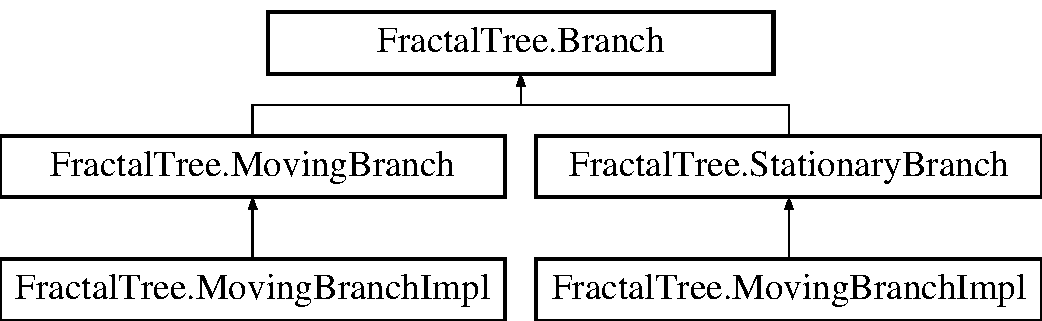
\includegraphics[height=3.000000cm]{interface_fractal_tree_1_1_branch}
\end{center}
\end{figure}
\subsection*{Public Member Functions}
\begin{DoxyCompactItemize}
\item 
void \hyperlink{interface_fractal_tree_1_1_branch_a1bad78362d67435aed4538b207f4155b}{Setup} (\hyperlink{interface_fractal_tree_1_1_branch}{Branch} owner, Vector2 end, float thickness, Color color)
\begin{DoxyCompactList}\small\item\em Setup the specified owner, end, thickness and color. Used to create a branch that is attached to another branch. \end{DoxyCompactList}\item 
void \hyperlink{interface_fractal_tree_1_1_branch_aac4a29be86256dff265190ed0d3ef250}{Setup} (\hyperlink{interface_fractal_tree_1_1_branch}{Branch} owner, Vector2 end, float thickness, Color color, bool auto\+Mass)
\begin{DoxyCompactList}\small\item\em Setup the specified owner, end, thickness and color. Used to create a branch that is attached to another branch that has its mass autogenerated based on line width. \end{DoxyCompactList}\item 
void \hyperlink{interface_fractal_tree_1_1_branch_a6c313c988c603a9d558871bd560a0b70}{Setup} (Vector2 start, Vector2 end, float thickness, Color color)
\begin{DoxyCompactList}\small\item\em Setup the specified start, end, thickness and color. Creates a stand alone branch that is not connected to any other branch. \end{DoxyCompactList}\item 
void \hyperlink{interface_fractal_tree_1_1_branch_ad813c22ae887cf465056d5eee5acb651}{Setup} (Vector2 start, Vector2 end, float width, Color color, bool auto\+Mass)
\begin{DoxyCompactList}\small\item\em Setup the specified start, end, thickness and color. Creates a stand alone branch that is not connected to any other branch that has its mass autogenerated based on line width. \end{DoxyCompactList}\item 
T \hyperlink{interface_fractal_tree_1_1_branch_ad3240d5e5d13df2ee22e55892f9c03cd}{Do\+Branching$<$ T $>$} (float angle)
\begin{DoxyCompactList}\small\item\em Returns a new branch based on current branch angle plus parameter angle. \end{DoxyCompactList}\item 
void \hyperlink{interface_fractal_tree_1_1_branch_a4460379e72ec587f890b1e0cf77dbc3c}{Do\+Colonization\+Reset} ()
\begin{DoxyCompactList}\small\item\em Resets the colonization paramater. Used only for space colonization generation. \end{DoxyCompactList}\end{DoxyCompactItemize}
\subsection*{Properties}
\begin{DoxyCompactItemize}
\item 
Vector2 \hyperlink{interface_fractal_tree_1_1_branch_a52b6d474fb483fb9e37e1c3fb8407ac5}{start\+Pos}\hspace{0.3cm}{\ttfamily  \mbox{[}get\mbox{]}}
\begin{DoxyCompactList}\small\item\em Gets the start position. \end{DoxyCompactList}\item 
Vector2 \hyperlink{interface_fractal_tree_1_1_branch_a5fb0f25128777e86c137a98958f3072b}{end\+Pos}\hspace{0.3cm}{\ttfamily  \mbox{[}get\mbox{]}}
\begin{DoxyCompactList}\small\item\em Gets the end position. \end{DoxyCompactList}\item 
Vector2 \hyperlink{interface_fractal_tree_1_1_branch_a1c83eb986e51a7c77b85b5d8dd68b8fc}{colonization\+Dir}\hspace{0.3cm}{\ttfamily  \mbox{[}get, set\mbox{]}}
\begin{DoxyCompactList}\small\item\em Gets or sets the colonization direction. Used for space colonization tree generation. Defines the direction of the next branch in relation to nearby leaves. \end{DoxyCompactList}\item 
int \hyperlink{interface_fractal_tree_1_1_branch_a218b95e107b90de1f7e0587a95c53afc}{colonization\+Leaf\+Count}\hspace{0.3cm}{\ttfamily  \mbox{[}get, set\mbox{]}}
\begin{DoxyCompactList}\small\item\em Gets or sets the number of nearby colonizaion leaves. \end{DoxyCompactList}\item 
bool \hyperlink{interface_fractal_tree_1_1_branch_a91cf75bd1bfc1d180be42ee4b461f3e8}{has\+Branched}\hspace{0.3cm}{\ttfamily  \mbox{[}get, set\mbox{]}}
\begin{DoxyCompactList}\small\item\em Gets or sets a value indicating whether this \hyperlink{interface_fractal_tree_1_1_branch}{Fractal\+Tree.\+Branch} has branched. \end{DoxyCompactList}\item 
Transform \hyperlink{interface_fractal_tree_1_1_branch_a4063cbfa57dfa91075a67c124ae3a3ac}{transform}\hspace{0.3cm}{\ttfamily  \mbox{[}get\mbox{]}}
\begin{DoxyCompactList}\small\item\em Gets the transform. \end{DoxyCompactList}\end{DoxyCompactItemize}


\subsection{Detailed Description}
Contract for all fractal tree branches. Includes positional data and initialisation. 



\subsection{Member Function Documentation}
\hypertarget{interface_fractal_tree_1_1_branch_ad3240d5e5d13df2ee22e55892f9c03cd}{}\label{interface_fractal_tree_1_1_branch_ad3240d5e5d13df2ee22e55892f9c03cd} 
\index{Fractal\+Tree\+::\+Branch@{Fractal\+Tree\+::\+Branch}!Do\+Branching$<$ T $>$@{Do\+Branching$<$ T $>$}}
\index{Do\+Branching$<$ T $>$@{Do\+Branching$<$ T $>$}!Fractal\+Tree\+::\+Branch@{Fractal\+Tree\+::\+Branch}}
\subsubsection{\texorpdfstring{Do\+Branching$<$ T $>$()}{DoBranching< T >()}}
{\footnotesize\ttfamily T Fractal\+Tree.\+Branch.\+Do\+Branching$<$ T $>$ (\begin{DoxyParamCaption}\item[{float}]{angle }\end{DoxyParamCaption})}



Returns a new branch based on current branch angle plus parameter angle. 

\begin{DoxyReturn}{Returns}
The branching.
\end{DoxyReturn}

\begin{DoxyParams}{Parameters}
{\em angle} & Angle.\\
\hline
\end{DoxyParams}

\begin{DoxyTemplParams}{Template Parameters}
{\em T} & The 1st type parameter.\\
\hline
\end{DoxyTemplParams}


Implemented in \hyperlink{class_fractal_tree_1_1_stationary_branch_a57ff42d0c4793c0c40aa1671905bf222}{Fractal\+Tree.\+Stationary\+Branch}, and \hyperlink{class_fractal_tree_1_1_moving_branch_impl_a7f7776446fa70aac8efb669f9e41a4af}{Fractal\+Tree.\+Moving\+Branch\+Impl}.

\begin{Desc}
\item[Type Constraints]\begin{description}
\item[{\em T} : {\em Branch}]\end{description}
\end{Desc}
\hypertarget{interface_fractal_tree_1_1_branch_a4460379e72ec587f890b1e0cf77dbc3c}{}\label{interface_fractal_tree_1_1_branch_a4460379e72ec587f890b1e0cf77dbc3c} 
\index{Fractal\+Tree\+::\+Branch@{Fractal\+Tree\+::\+Branch}!Do\+Colonization\+Reset@{Do\+Colonization\+Reset}}
\index{Do\+Colonization\+Reset@{Do\+Colonization\+Reset}!Fractal\+Tree\+::\+Branch@{Fractal\+Tree\+::\+Branch}}
\subsubsection{\texorpdfstring{Do\+Colonization\+Reset()}{DoColonizationReset()}}
{\footnotesize\ttfamily void Fractal\+Tree.\+Branch.\+Do\+Colonization\+Reset (\begin{DoxyParamCaption}{ }\end{DoxyParamCaption})}



Resets the colonization paramater. Used only for space colonization generation. 



Implemented in \hyperlink{class_fractal_tree_1_1_stationary_branch_a57a5b1cbc9fd081c5b8cb41b61d24502}{Fractal\+Tree.\+Stationary\+Branch}.

\hypertarget{interface_fractal_tree_1_1_branch_a1bad78362d67435aed4538b207f4155b}{}\label{interface_fractal_tree_1_1_branch_a1bad78362d67435aed4538b207f4155b} 
\index{Fractal\+Tree\+::\+Branch@{Fractal\+Tree\+::\+Branch}!Setup@{Setup}}
\index{Setup@{Setup}!Fractal\+Tree\+::\+Branch@{Fractal\+Tree\+::\+Branch}}
\subsubsection{\texorpdfstring{Setup()}{Setup()}\hspace{0.1cm}{\footnotesize\ttfamily [1/4]}}
{\footnotesize\ttfamily void Fractal\+Tree.\+Branch.\+Setup (\begin{DoxyParamCaption}\item[{\hyperlink{interface_fractal_tree_1_1_branch}{Branch}}]{owner,  }\item[{Vector2}]{end,  }\item[{float}]{thickness,  }\item[{Color}]{color }\end{DoxyParamCaption})}



Setup the specified owner, end, thickness and color. Used to create a branch that is attached to another branch. 


\begin{DoxyParams}{Parameters}
{\em owner} & The attached branch.\\
\hline
{\em end} & End.\\
\hline
{\em thickness} & Thickness.\\
\hline
{\em color} & Color.\\
\hline
\end{DoxyParams}


Implemented in \hyperlink{class_fractal_tree_1_1_stationary_branch_acaa0bef74389db9f1a2f57af38557000}{Fractal\+Tree.\+Stationary\+Branch}, and \hyperlink{class_fractal_tree_1_1_moving_branch_impl_a52861b34bb8a9550c6790bab90509660}{Fractal\+Tree.\+Moving\+Branch\+Impl}.

\hypertarget{interface_fractal_tree_1_1_branch_aac4a29be86256dff265190ed0d3ef250}{}\label{interface_fractal_tree_1_1_branch_aac4a29be86256dff265190ed0d3ef250} 
\index{Fractal\+Tree\+::\+Branch@{Fractal\+Tree\+::\+Branch}!Setup@{Setup}}
\index{Setup@{Setup}!Fractal\+Tree\+::\+Branch@{Fractal\+Tree\+::\+Branch}}
\subsubsection{\texorpdfstring{Setup()}{Setup()}\hspace{0.1cm}{\footnotesize\ttfamily [2/4]}}
{\footnotesize\ttfamily void Fractal\+Tree.\+Branch.\+Setup (\begin{DoxyParamCaption}\item[{\hyperlink{interface_fractal_tree_1_1_branch}{Branch}}]{owner,  }\item[{Vector2}]{end,  }\item[{float}]{thickness,  }\item[{Color}]{color,  }\item[{bool}]{auto\+Mass }\end{DoxyParamCaption})}



Setup the specified owner, end, thickness and color. Used to create a branch that is attached to another branch that has its mass autogenerated based on line width. 


\begin{DoxyParams}{Parameters}
{\em owner} & Owner.\\
\hline
{\em end} & End.\\
\hline
{\em thickness} & Thickness.\\
\hline
{\em color} & Color.\\
\hline
{\em auto\+Mass} & If set to {\ttfamily true} auto mass.\\
\hline
\end{DoxyParams}


Implemented in \hyperlink{class_fractal_tree_1_1_stationary_branch_a262c5810fadbd2c8aea1f2afdca57126}{Fractal\+Tree.\+Stationary\+Branch}, and \hyperlink{class_fractal_tree_1_1_moving_branch_impl_a73649451c7fbfa0793e0a1528e301215}{Fractal\+Tree.\+Moving\+Branch\+Impl}.

\hypertarget{interface_fractal_tree_1_1_branch_a6c313c988c603a9d558871bd560a0b70}{}\label{interface_fractal_tree_1_1_branch_a6c313c988c603a9d558871bd560a0b70} 
\index{Fractal\+Tree\+::\+Branch@{Fractal\+Tree\+::\+Branch}!Setup@{Setup}}
\index{Setup@{Setup}!Fractal\+Tree\+::\+Branch@{Fractal\+Tree\+::\+Branch}}
\subsubsection{\texorpdfstring{Setup()}{Setup()}\hspace{0.1cm}{\footnotesize\ttfamily [3/4]}}
{\footnotesize\ttfamily void Fractal\+Tree.\+Branch.\+Setup (\begin{DoxyParamCaption}\item[{Vector2}]{start,  }\item[{Vector2}]{end,  }\item[{float}]{thickness,  }\item[{Color}]{color }\end{DoxyParamCaption})}



Setup the specified start, end, thickness and color. Creates a stand alone branch that is not connected to any other branch. 


\begin{DoxyParams}{Parameters}
{\em start} & Start.\\
\hline
{\em end} & End.\\
\hline
{\em thickness} & Thickness.\\
\hline
{\em color} & Color.\\
\hline
\end{DoxyParams}


Implemented in \hyperlink{class_fractal_tree_1_1_stationary_branch_a62e1aa7062ef70a8726dfe21a9e28d76}{Fractal\+Tree.\+Stationary\+Branch}, and \hyperlink{class_fractal_tree_1_1_moving_branch_impl_aeea52b05117e613e0dd6c9ee5fbafb58}{Fractal\+Tree.\+Moving\+Branch\+Impl}.

\hypertarget{interface_fractal_tree_1_1_branch_ad813c22ae887cf465056d5eee5acb651}{}\label{interface_fractal_tree_1_1_branch_ad813c22ae887cf465056d5eee5acb651} 
\index{Fractal\+Tree\+::\+Branch@{Fractal\+Tree\+::\+Branch}!Setup@{Setup}}
\index{Setup@{Setup}!Fractal\+Tree\+::\+Branch@{Fractal\+Tree\+::\+Branch}}
\subsubsection{\texorpdfstring{Setup()}{Setup()}\hspace{0.1cm}{\footnotesize\ttfamily [4/4]}}
{\footnotesize\ttfamily void Fractal\+Tree.\+Branch.\+Setup (\begin{DoxyParamCaption}\item[{Vector2}]{start,  }\item[{Vector2}]{end,  }\item[{float}]{width,  }\item[{Color}]{color,  }\item[{bool}]{auto\+Mass }\end{DoxyParamCaption})}



Setup the specified start, end, thickness and color. Creates a stand alone branch that is not connected to any other branch that has its mass autogenerated based on line width. 


\begin{DoxyParams}{Parameters}
{\em start} & Start.\\
\hline
{\em end} & End.\\
\hline
{\em width} & Width.\\
\hline
{\em color} & Color.\\
\hline
{\em auto\+Mass} & If set to {\ttfamily true} auto mass.\\
\hline
\end{DoxyParams}


Implemented in \hyperlink{class_fractal_tree_1_1_stationary_branch_a61cfd43bb83cf63bf1ad25f339866d7a}{Fractal\+Tree.\+Stationary\+Branch}, and \hyperlink{class_fractal_tree_1_1_moving_branch_impl_a4e7cde65899abaf121a906d06874c330}{Fractal\+Tree.\+Moving\+Branch\+Impl}.



\subsection{Property Documentation}
\hypertarget{interface_fractal_tree_1_1_branch_a1c83eb986e51a7c77b85b5d8dd68b8fc}{}\label{interface_fractal_tree_1_1_branch_a1c83eb986e51a7c77b85b5d8dd68b8fc} 
\index{Fractal\+Tree\+::\+Branch@{Fractal\+Tree\+::\+Branch}!colonization\+Dir@{colonization\+Dir}}
\index{colonization\+Dir@{colonization\+Dir}!Fractal\+Tree\+::\+Branch@{Fractal\+Tree\+::\+Branch}}
\subsubsection{\texorpdfstring{colonization\+Dir}{colonizationDir}}
{\footnotesize\ttfamily Vector2 Fractal\+Tree.\+Branch.\+colonization\+Dir\hspace{0.3cm}{\ttfamily [get]}, {\ttfamily [set]}}



Gets or sets the colonization direction. Used for space colonization tree generation. Defines the direction of the next branch in relation to nearby leaves. 

The colonization dir.\hypertarget{interface_fractal_tree_1_1_branch_a218b95e107b90de1f7e0587a95c53afc}{}\label{interface_fractal_tree_1_1_branch_a218b95e107b90de1f7e0587a95c53afc} 
\index{Fractal\+Tree\+::\+Branch@{Fractal\+Tree\+::\+Branch}!colonization\+Leaf\+Count@{colonization\+Leaf\+Count}}
\index{colonization\+Leaf\+Count@{colonization\+Leaf\+Count}!Fractal\+Tree\+::\+Branch@{Fractal\+Tree\+::\+Branch}}
\subsubsection{\texorpdfstring{colonization\+Leaf\+Count}{colonizationLeafCount}}
{\footnotesize\ttfamily int Fractal\+Tree.\+Branch.\+colonization\+Leaf\+Count\hspace{0.3cm}{\ttfamily [get]}, {\ttfamily [set]}}



Gets or sets the number of nearby colonizaion leaves. 

The colonization leaf count.\hypertarget{interface_fractal_tree_1_1_branch_a5fb0f25128777e86c137a98958f3072b}{}\label{interface_fractal_tree_1_1_branch_a5fb0f25128777e86c137a98958f3072b} 
\index{Fractal\+Tree\+::\+Branch@{Fractal\+Tree\+::\+Branch}!end\+Pos@{end\+Pos}}
\index{end\+Pos@{end\+Pos}!Fractal\+Tree\+::\+Branch@{Fractal\+Tree\+::\+Branch}}
\subsubsection{\texorpdfstring{end\+Pos}{endPos}}
{\footnotesize\ttfamily Vector2 Fractal\+Tree.\+Branch.\+end\+Pos\hspace{0.3cm}{\ttfamily [get]}}



Gets the end position. 

The end position.\hypertarget{interface_fractal_tree_1_1_branch_a91cf75bd1bfc1d180be42ee4b461f3e8}{}\label{interface_fractal_tree_1_1_branch_a91cf75bd1bfc1d180be42ee4b461f3e8} 
\index{Fractal\+Tree\+::\+Branch@{Fractal\+Tree\+::\+Branch}!has\+Branched@{has\+Branched}}
\index{has\+Branched@{has\+Branched}!Fractal\+Tree\+::\+Branch@{Fractal\+Tree\+::\+Branch}}
\subsubsection{\texorpdfstring{has\+Branched}{hasBranched}}
{\footnotesize\ttfamily bool Fractal\+Tree.\+Branch.\+has\+Branched\hspace{0.3cm}{\ttfamily [get]}, {\ttfamily [set]}}



Gets or sets a value indicating whether this \hyperlink{interface_fractal_tree_1_1_branch}{Fractal\+Tree.\+Branch} has branched. 

{\ttfamily true} if has branched; otherwise, {\ttfamily false}.\hypertarget{interface_fractal_tree_1_1_branch_a52b6d474fb483fb9e37e1c3fb8407ac5}{}\label{interface_fractal_tree_1_1_branch_a52b6d474fb483fb9e37e1c3fb8407ac5} 
\index{Fractal\+Tree\+::\+Branch@{Fractal\+Tree\+::\+Branch}!start\+Pos@{start\+Pos}}
\index{start\+Pos@{start\+Pos}!Fractal\+Tree\+::\+Branch@{Fractal\+Tree\+::\+Branch}}
\subsubsection{\texorpdfstring{start\+Pos}{startPos}}
{\footnotesize\ttfamily Vector2 Fractal\+Tree.\+Branch.\+start\+Pos\hspace{0.3cm}{\ttfamily [get]}}



Gets the start position. 

The start position.\hypertarget{interface_fractal_tree_1_1_branch_a4063cbfa57dfa91075a67c124ae3a3ac}{}\label{interface_fractal_tree_1_1_branch_a4063cbfa57dfa91075a67c124ae3a3ac} 
\index{Fractal\+Tree\+::\+Branch@{Fractal\+Tree\+::\+Branch}!transform@{transform}}
\index{transform@{transform}!Fractal\+Tree\+::\+Branch@{Fractal\+Tree\+::\+Branch}}
\subsubsection{\texorpdfstring{transform}{transform}}
{\footnotesize\ttfamily Transform Fractal\+Tree.\+Branch.\+transform\hspace{0.3cm}{\ttfamily [get]}}



Gets the transform. 

The transform.

The documentation for this interface was generated from the following file\+:\begin{DoxyCompactItemize}
\item 
Branch.\+cs\end{DoxyCompactItemize}

\hypertarget{class_fractal_tree_1_1_colonization_leaf}{}\section{Fractal\+Tree.\+Colonization\+Leaf Class Reference}
\label{class_fractal_tree_1_1_colonization_leaf}\index{Fractal\+Tree.\+Colonization\+Leaf@{Fractal\+Tree.\+Colonization\+Leaf}}


Attach to leaf objects for space colonization. The branches move towards the leaves.  


Inheritance diagram for Fractal\+Tree.\+Colonization\+Leaf\+:\begin{figure}[H]
\begin{center}
\leavevmode
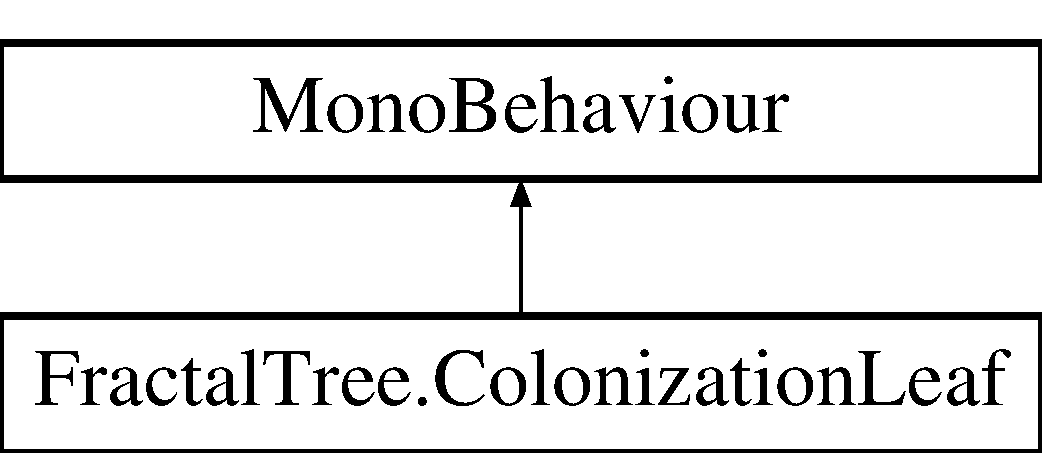
\includegraphics[height=2.000000cm]{class_fractal_tree_1_1_colonization_leaf}
\end{center}
\end{figure}
\subsection*{Properties}
\begin{DoxyCompactItemize}
\item 
bool \hyperlink{class_fractal_tree_1_1_colonization_leaf_ad45a7ad00f87add9c92cd78047e892aa}{has\+Been\+Reached}\hspace{0.3cm}{\ttfamily  \mbox{[}get, set\mbox{]}}
\begin{DoxyCompactList}\small\item\em Within the minimum distance of a branch. To be removed from the simulation. \end{DoxyCompactList}\item 
Vector2 \hyperlink{class_fractal_tree_1_1_colonization_leaf_a3e33ba00c3c7536f51f7f0c71487a091}{position}\hspace{0.3cm}{\ttfamily  \mbox{[}get\mbox{]}}
\begin{DoxyCompactList}\small\item\em Gets the position of the leaf. \end{DoxyCompactList}\end{DoxyCompactItemize}


\subsection{Detailed Description}
Attach to leaf objects for space colonization. The branches move towards the leaves. 



\subsection{Property Documentation}
\mbox{\Hypertarget{class_fractal_tree_1_1_colonization_leaf_ad45a7ad00f87add9c92cd78047e892aa}\label{class_fractal_tree_1_1_colonization_leaf_ad45a7ad00f87add9c92cd78047e892aa}} 
\index{Fractal\+Tree\+::\+Colonization\+Leaf@{Fractal\+Tree\+::\+Colonization\+Leaf}!has\+Been\+Reached@{has\+Been\+Reached}}
\index{has\+Been\+Reached@{has\+Been\+Reached}!Fractal\+Tree\+::\+Colonization\+Leaf@{Fractal\+Tree\+::\+Colonization\+Leaf}}
\subsubsection{\texorpdfstring{has\+Been\+Reached}{hasBeenReached}}
{\footnotesize\ttfamily bool Fractal\+Tree.\+Colonization\+Leaf.\+has\+Been\+Reached\hspace{0.3cm}{\ttfamily [get]}, {\ttfamily [set]}}



Within the minimum distance of a branch. To be removed from the simulation. 

{\ttfamily true} if has been reached; otherwise, {\ttfamily false}.\mbox{\Hypertarget{class_fractal_tree_1_1_colonization_leaf_a3e33ba00c3c7536f51f7f0c71487a091}\label{class_fractal_tree_1_1_colonization_leaf_a3e33ba00c3c7536f51f7f0c71487a091}} 
\index{Fractal\+Tree\+::\+Colonization\+Leaf@{Fractal\+Tree\+::\+Colonization\+Leaf}!position@{position}}
\index{position@{position}!Fractal\+Tree\+::\+Colonization\+Leaf@{Fractal\+Tree\+::\+Colonization\+Leaf}}
\subsubsection{\texorpdfstring{position}{position}}
{\footnotesize\ttfamily Vector2 Fractal\+Tree.\+Colonization\+Leaf.\+position\hspace{0.3cm}{\ttfamily [get]}}



Gets the position of the leaf. 

The position.

The documentation for this class was generated from the following file\+:\begin{DoxyCompactItemize}
\item 
F\+T/\+Scripts/\+Trees/Colonization\+Leaf.\+cs\end{DoxyCompactItemize}

\hypertarget{class_fractal_tree_1_1_colonization_leaf_generator}{}\section{Fractal\+Tree.\+Colonization\+Leaf\+Generator Class Reference}
\label{class_fractal_tree_1_1_colonization_leaf_generator}\index{Fractal\+Tree.\+Colonization\+Leaf\+Generator@{Fractal\+Tree.\+Colonization\+Leaf\+Generator}}


Spawns a set number of leaves within a bounds. Used by space colonization.  


Inheritance diagram for Fractal\+Tree.\+Colonization\+Leaf\+Generator\+:\begin{figure}[H]
\begin{center}
\leavevmode
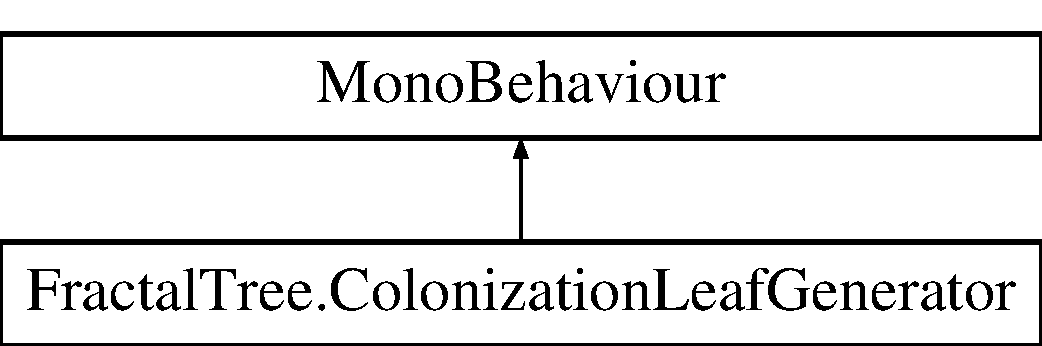
\includegraphics[height=2.000000cm]{class_fractal_tree_1_1_colonization_leaf_generator}
\end{center}
\end{figure}
\subsection*{Public Member Functions}
\begin{DoxyCompactItemize}
\item 
\mbox{\Hypertarget{class_fractal_tree_1_1_colonization_leaf_generator_afd290e9cb003f9b58ad596a1a9920491}\label{class_fractal_tree_1_1_colonization_leaf_generator_afd290e9cb003f9b58ad596a1a9920491}} 
void {\bfseries Generate} ()
\item 
\mbox{\Hypertarget{class_fractal_tree_1_1_colonization_leaf_generator_a01c5ac8c4629f855787aba4cafa6dd57}\label{class_fractal_tree_1_1_colonization_leaf_generator_a01c5ac8c4629f855787aba4cafa6dd57}} 
void {\bfseries Remove} ()
\end{DoxyCompactItemize}
\subsection*{Public Attributes}
\begin{DoxyCompactItemize}
\item 
\mbox{\Hypertarget{class_fractal_tree_1_1_colonization_leaf_generator_aca372b1936473828af2109bae812fd1a}\label{class_fractal_tree_1_1_colonization_leaf_generator_aca372b1936473828af2109bae812fd1a}} 
float {\bfseries radius} = 6f
\item 
int \hyperlink{class_fractal_tree_1_1_colonization_leaf_generator_a8c80eb30ad9f225f5e5d146f8b633e0c}{num\+To\+Create} = 100
\begin{DoxyCompactList}\small\item\em The number of leaves to spawn. \end{DoxyCompactList}\item 
\mbox{\Hypertarget{class_fractal_tree_1_1_colonization_leaf_generator_afff155fcf2579e3aaf074abe59bb0b0f}\label{class_fractal_tree_1_1_colonization_leaf_generator_afff155fcf2579e3aaf074abe59bb0b0f}} 
bool {\bfseries build\+On\+Start} = false
\end{DoxyCompactItemize}


\subsection{Detailed Description}
Spawns a set number of leaves within a bounds. Used by space colonization. 



\subsection{Member Data Documentation}
\mbox{\Hypertarget{class_fractal_tree_1_1_colonization_leaf_generator_a8c80eb30ad9f225f5e5d146f8b633e0c}\label{class_fractal_tree_1_1_colonization_leaf_generator_a8c80eb30ad9f225f5e5d146f8b633e0c}} 
\index{Fractal\+Tree\+::\+Colonization\+Leaf\+Generator@{Fractal\+Tree\+::\+Colonization\+Leaf\+Generator}!num\+To\+Create@{num\+To\+Create}}
\index{num\+To\+Create@{num\+To\+Create}!Fractal\+Tree\+::\+Colonization\+Leaf\+Generator@{Fractal\+Tree\+::\+Colonization\+Leaf\+Generator}}
\subsubsection{\texorpdfstring{num\+To\+Create}{numToCreate}}
{\footnotesize\ttfamily int Fractal\+Tree.\+Colonization\+Leaf\+Generator.\+num\+To\+Create = 100}



The number of leaves to spawn. 



The documentation for this class was generated from the following file\+:\begin{DoxyCompactItemize}
\item 
F\+T/\+Scripts/\+Trees/Colonization\+Leaf\+Generator.\+cs\end{DoxyCompactItemize}

\hypertarget{class_fractal_tree_1_1_colonization_tree}{}\section{Fractal\+Tree.\+Colonization\+Tree Class Reference}
\label{class_fractal_tree_1_1_colonization_tree}\index{Fractal\+Tree.\+Colonization\+Tree@{Fractal\+Tree.\+Colonization\+Tree}}


Spawns a fractal tree using space colonization\+: \href{http://algorithmicbotany.org/papers/colonization.egwnp2007.pdf}{\tt http\+://algorithmicbotany.\+org/papers/colonization.\+egwnp2007.\+pdf}  


Inheritance diagram for Fractal\+Tree.\+Colonization\+Tree\+:\begin{figure}[H]
\begin{center}
\leavevmode
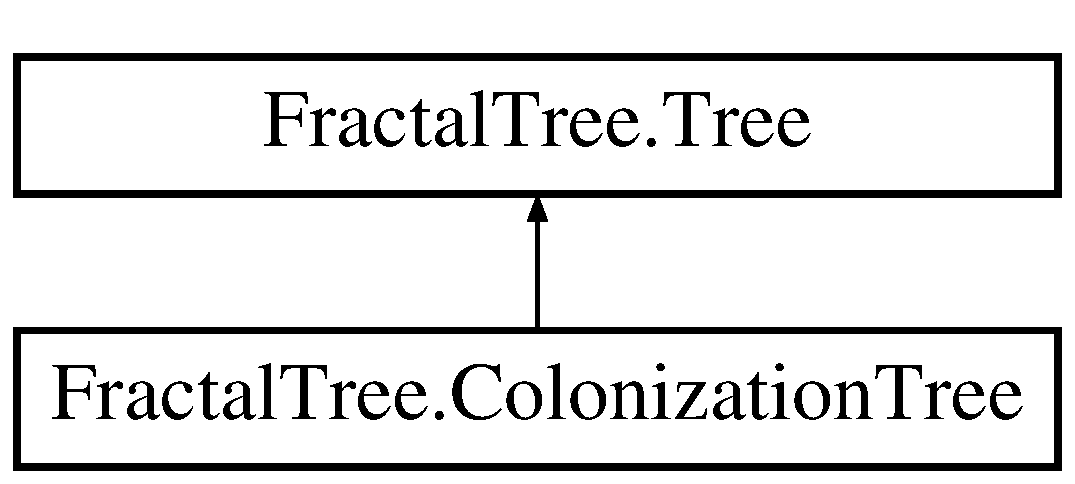
\includegraphics[height=2.000000cm]{class_fractal_tree_1_1_colonization_tree}
\end{center}
\end{figure}
\subsection*{Public Member Functions}
\begin{DoxyCompactItemize}
\item 
\hyperlink{class_fractal_tree_1_1_colonization_tree_acba99f382cef3e5184f0558dd5a089ea}{Colonization\+Tree} (List$<$ \hyperlink{class_fractal_tree_1_1_colonization_leaf}{Colonization\+Leaf} $>$ leaves, Transform owner, float initial\+Length, Game\+Object branch\+Prefab, float width, float min\+Distance, float max\+Distance)
\begin{DoxyCompactList}\small\item\em Initializes a new instance of the \hyperlink{class_fractal_tree_1_1_colonization_tree}{Fractal\+Tree.\+Colonization\+Tree} class. \end{DoxyCompactList}\item 
List$<$ T $>$ \hyperlink{class_fractal_tree_1_1_colonization_tree_ac16d379a8d3c2f2a56ef5e3f1c66df36}{Generate$<$ T $>$} ()
\begin{DoxyCompactList}\small\item\em Generates a tree using space colonization. \end{DoxyCompactList}\end{DoxyCompactItemize}


\subsection{Detailed Description}
Spawns a fractal tree using space colonization\+: \href{http://algorithmicbotany.org/papers/colonization.egwnp2007.pdf}{\tt http\+://algorithmicbotany.\+org/papers/colonization.\+egwnp2007.\+pdf} 



\subsection{Constructor \& Destructor Documentation}
\hypertarget{class_fractal_tree_1_1_colonization_tree_acba99f382cef3e5184f0558dd5a089ea}{}\label{class_fractal_tree_1_1_colonization_tree_acba99f382cef3e5184f0558dd5a089ea} 
\index{Fractal\+Tree\+::\+Colonization\+Tree@{Fractal\+Tree\+::\+Colonization\+Tree}!Colonization\+Tree@{Colonization\+Tree}}
\index{Colonization\+Tree@{Colonization\+Tree}!Fractal\+Tree\+::\+Colonization\+Tree@{Fractal\+Tree\+::\+Colonization\+Tree}}
\subsubsection{\texorpdfstring{Colonization\+Tree()}{ColonizationTree()}}
{\footnotesize\ttfamily Fractal\+Tree.\+Colonization\+Tree.\+Colonization\+Tree (\begin{DoxyParamCaption}\item[{List$<$ \hyperlink{class_fractal_tree_1_1_colonization_leaf}{Colonization\+Leaf} $>$}]{leaves,  }\item[{Transform}]{owner,  }\item[{float}]{initial\+Length,  }\item[{Game\+Object}]{branch\+Prefab,  }\item[{float}]{width,  }\item[{float}]{min\+Distance,  }\item[{float}]{max\+Distance }\end{DoxyParamCaption})}



Initializes a new instance of the \hyperlink{class_fractal_tree_1_1_colonization_tree}{Fractal\+Tree.\+Colonization\+Tree} class. 


\begin{DoxyParams}{Parameters}
{\em leaves} & Leaves.\\
\hline
{\em owner} & Owner.\\
\hline
{\em initial\+Length} & Initial length.\\
\hline
{\em branch\+Prefab} & \hyperlink{interface_fractal_tree_1_1_branch}{Branch} prefab.\\
\hline
{\em width} & Width.\\
\hline
{\em min\+Distance} & Minimum distance.\\
\hline
{\em max\+Distance} & Max distance.\\
\hline
\end{DoxyParams}


\subsection{Member Function Documentation}
\hypertarget{class_fractal_tree_1_1_colonization_tree_ac16d379a8d3c2f2a56ef5e3f1c66df36}{}\label{class_fractal_tree_1_1_colonization_tree_ac16d379a8d3c2f2a56ef5e3f1c66df36} 
\index{Fractal\+Tree\+::\+Colonization\+Tree@{Fractal\+Tree\+::\+Colonization\+Tree}!Generate$<$ T $>$@{Generate$<$ T $>$}}
\index{Generate$<$ T $>$@{Generate$<$ T $>$}!Fractal\+Tree\+::\+Colonization\+Tree@{Fractal\+Tree\+::\+Colonization\+Tree}}
\subsubsection{\texorpdfstring{Generate$<$ T $>$()}{Generate< T >()}}
{\footnotesize\ttfamily List$<$T$>$ Fractal\+Tree.\+Colonization\+Tree.\+Generate$<$ T $>$ (\begin{DoxyParamCaption}{ }\end{DoxyParamCaption})}



Generates a tree using space colonization. 


\begin{DoxyTemplParams}{Template Parameters}
{\em T} & \hyperlink{interface_fractal_tree_1_1_branch}{Branch} type.\\
\hline
\end{DoxyTemplParams}


Implements \hyperlink{interface_fractal_tree_1_1_tree}{Fractal\+Tree.\+Tree}.

\begin{Desc}
\item[Type Constraints]\begin{description}
\item[{\em T} : {\em Branch}]\end{description}
\end{Desc}


The documentation for this class was generated from the following file\+:\begin{DoxyCompactItemize}
\item 
Colonization\+Tree.\+cs\end{DoxyCompactItemize}

\hypertarget{class_fractal_tree_1_1_default_tree}{}\section{Fractal\+Tree.\+Default\+Tree Class Reference}
\label{class_fractal_tree_1_1_default_tree}\index{Fractal\+Tree.\+Default\+Tree@{Fractal\+Tree.\+Default\+Tree}}


Spawns a fractal tree.  


Inheritance diagram for Fractal\+Tree.\+Default\+Tree\+:\begin{figure}[H]
\begin{center}
\leavevmode
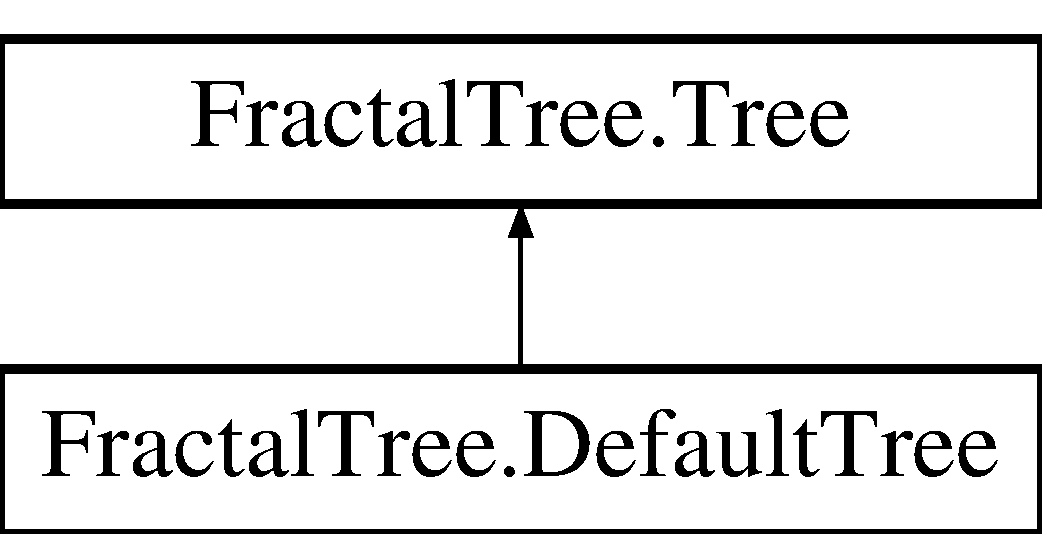
\includegraphics[height=2.000000cm]{class_fractal_tree_1_1_default_tree}
\end{center}
\end{figure}
\subsection*{Public Member Functions}
\begin{DoxyCompactItemize}
\item 
\hyperlink{class_fractal_tree_1_1_default_tree_adf83fe3bdb427d26f3353eaf069906fb}{Default\+Tree} (int growth, float initial\+Length, float length\+Degredation, float angle, float thickness, Game\+Object branch\+Prefab, Color branch\+Color, Transform owner)
\begin{DoxyCompactList}\small\item\em Initializes a new instance of the \hyperlink{class_fractal_tree_1_1_default_tree}{Fractal\+Tree.\+Default\+Tree} class. \end{DoxyCompactList}\item 
List$<$ T $>$ \hyperlink{class_fractal_tree_1_1_default_tree_a99f8ba1f24ba5693f0981be567b236a0}{Generate$<$ T $>$} ()
\begin{DoxyCompactList}\small\item\em Generates a fractal tree. \end{DoxyCompactList}\end{DoxyCompactItemize}


\subsection{Detailed Description}
Spawns a fractal tree. 



\subsection{Constructor \& Destructor Documentation}
\mbox{\Hypertarget{class_fractal_tree_1_1_default_tree_adf83fe3bdb427d26f3353eaf069906fb}\label{class_fractal_tree_1_1_default_tree_adf83fe3bdb427d26f3353eaf069906fb}} 
\index{Fractal\+Tree\+::\+Default\+Tree@{Fractal\+Tree\+::\+Default\+Tree}!Default\+Tree@{Default\+Tree}}
\index{Default\+Tree@{Default\+Tree}!Fractal\+Tree\+::\+Default\+Tree@{Fractal\+Tree\+::\+Default\+Tree}}
\subsubsection{\texorpdfstring{Default\+Tree()}{DefaultTree()}}
{\footnotesize\ttfamily Fractal\+Tree.\+Default\+Tree.\+Default\+Tree (\begin{DoxyParamCaption}\item[{int}]{growth,  }\item[{float}]{initial\+Length,  }\item[{float}]{length\+Degredation,  }\item[{float}]{angle,  }\item[{float}]{thickness,  }\item[{Game\+Object}]{branch\+Prefab,  }\item[{Color}]{branch\+Color,  }\item[{Transform}]{owner }\end{DoxyParamCaption})}



Initializes a new instance of the \hyperlink{class_fractal_tree_1_1_default_tree}{Fractal\+Tree.\+Default\+Tree} class. 


\begin{DoxyParams}{Parameters}
{\em growth} & Growth.\\
\hline
{\em initial\+Length} & Initial length.\\
\hline
{\em length\+Degredation} & Length degredation.\\
\hline
{\em angle} & Angle.\\
\hline
{\em thickness} & Thickness.\\
\hline
{\em branch\+Prefab} & \hyperlink{interface_fractal_tree_1_1_branch}{Branch} prefab.\\
\hline
{\em owner} & Owner.\\
\hline
\end{DoxyParams}


\subsection{Member Function Documentation}
\mbox{\Hypertarget{class_fractal_tree_1_1_default_tree_a99f8ba1f24ba5693f0981be567b236a0}\label{class_fractal_tree_1_1_default_tree_a99f8ba1f24ba5693f0981be567b236a0}} 
\index{Fractal\+Tree\+::\+Default\+Tree@{Fractal\+Tree\+::\+Default\+Tree}!Generate$<$ T $>$@{Generate$<$ T $>$}}
\index{Generate$<$ T $>$@{Generate$<$ T $>$}!Fractal\+Tree\+::\+Default\+Tree@{Fractal\+Tree\+::\+Default\+Tree}}
\subsubsection{\texorpdfstring{Generate$<$ T $>$()}{Generate< T >()}}
{\footnotesize\ttfamily List$<$T$>$ Fractal\+Tree.\+Default\+Tree.\+Generate$<$ T $>$ (\begin{DoxyParamCaption}{ }\end{DoxyParamCaption})}



Generates a fractal tree. 


\begin{DoxyTemplParams}{Template Parameters}
{\em T} & The 1st type parameter.\\
\hline
\end{DoxyTemplParams}


Implements \hyperlink{interface_fractal_tree_1_1_tree}{Fractal\+Tree.\+Tree}.

\begin{Desc}
\item[Type Constraints]\begin{description}
\item[{\em T} : {\em Branch}]\end{description}
\end{Desc}


The documentation for this class was generated from the following file\+:\begin{DoxyCompactItemize}
\item 
F\+T/\+Scripts/\+Trees/Default\+Tree.\+cs\end{DoxyCompactItemize}

\hypertarget{class_fractal_tree_1_1_demo_1_1_demo_branch_tree_u_i}{}\section{Fractal\+Tree.\+Demo.\+Demo\+Branch\+Tree\+UI Class Reference}
\label{class_fractal_tree_1_1_demo_1_1_demo_branch_tree_u_i}\index{Fractal\+Tree.\+Demo.\+Demo\+Branch\+Tree\+UI@{Fractal\+Tree.\+Demo.\+Demo\+Branch\+Tree\+UI}}


For demo purposes. Listens for changes in UI and updates \hyperlink{interface_fractal_tree_1_1_branch}{Branch} variables.  


Inheritance diagram for Fractal\+Tree.\+Demo.\+Demo\+Branch\+Tree\+UI\+:\begin{figure}[H]
\begin{center}
\leavevmode
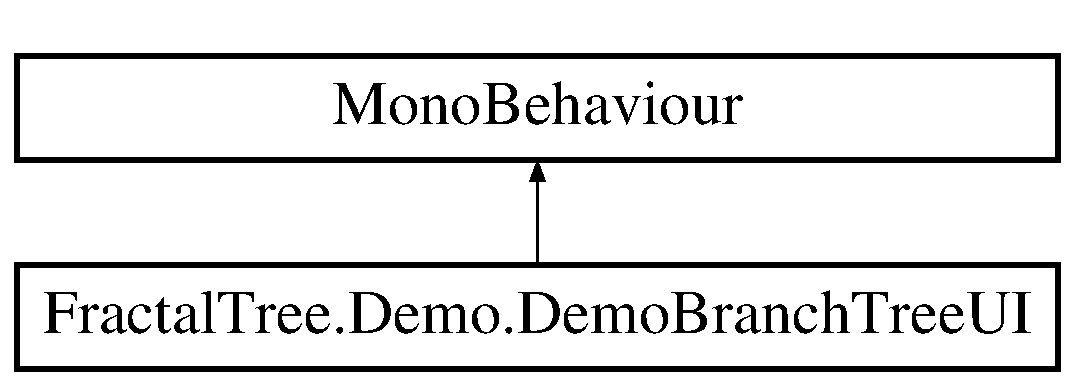
\includegraphics[height=2.000000cm]{class_fractal_tree_1_1_demo_1_1_demo_branch_tree_u_i}
\end{center}
\end{figure}
\subsection*{Public Member Functions}
\begin{DoxyCompactItemize}
\item 
\mbox{\Hypertarget{class_fractal_tree_1_1_demo_1_1_demo_branch_tree_u_i_a88791b1a9f6520af850c66f0f6cc2926}\label{class_fractal_tree_1_1_demo_1_1_demo_branch_tree_u_i_a88791b1a9f6520af850c66f0f6cc2926}} 
void {\bfseries On\+Generation\+Change} (string value)
\item 
\mbox{\Hypertarget{class_fractal_tree_1_1_demo_1_1_demo_branch_tree_u_i_a7ce65993febe8af23be5a5e4981b9d1f}\label{class_fractal_tree_1_1_demo_1_1_demo_branch_tree_u_i_a7ce65993febe8af23be5a5e4981b9d1f}} 
void {\bfseries On\+Length\+Changed} (string value)
\item 
\mbox{\Hypertarget{class_fractal_tree_1_1_demo_1_1_demo_branch_tree_u_i_a3a103511a8943b59384a3c9a3dad76fb}\label{class_fractal_tree_1_1_demo_1_1_demo_branch_tree_u_i_a3a103511a8943b59384a3c9a3dad76fb}} 
void {\bfseries On\+Multiplier\+Changed} (string value)
\item 
\mbox{\Hypertarget{class_fractal_tree_1_1_demo_1_1_demo_branch_tree_u_i_ad018096f974248845022b5db73a30186}\label{class_fractal_tree_1_1_demo_1_1_demo_branch_tree_u_i_ad018096f974248845022b5db73a30186}} 
void {\bfseries On\+Angle\+Changed} (string value)
\item 
\mbox{\Hypertarget{class_fractal_tree_1_1_demo_1_1_demo_branch_tree_u_i_a596eb53e29556c4bbe66612d3451888b}\label{class_fractal_tree_1_1_demo_1_1_demo_branch_tree_u_i_a596eb53e29556c4bbe66612d3451888b}} 
void {\bfseries On\+Width\+Changed} (string value)
\item 
\mbox{\Hypertarget{class_fractal_tree_1_1_demo_1_1_demo_branch_tree_u_i_a2a958e5e762329adb7fe58325aa25bb5}\label{class_fractal_tree_1_1_demo_1_1_demo_branch_tree_u_i_a2a958e5e762329adb7fe58325aa25bb5}} 
void {\bfseries Generate} ()
\end{DoxyCompactItemize}
\subsection*{Public Attributes}
\begin{DoxyCompactItemize}
\item 
\mbox{\Hypertarget{class_fractal_tree_1_1_demo_1_1_demo_branch_tree_u_i_afdab251ab27e57fa924df3baea2d1640}\label{class_fractal_tree_1_1_demo_1_1_demo_branch_tree_u_i_afdab251ab27e57fa924df3baea2d1640}} 
\hyperlink{class_fractal_tree_1_1_tree_builder}{Tree\+Builder} {\bfseries tree\+Builder}
\item 
\mbox{\Hypertarget{class_fractal_tree_1_1_demo_1_1_demo_branch_tree_u_i_ab33f8bffbc27cc63893399be2ac52d7e}\label{class_fractal_tree_1_1_demo_1_1_demo_branch_tree_u_i_ab33f8bffbc27cc63893399be2ac52d7e}} 
Input\+Field {\bfseries gen\+Input}
\item 
\mbox{\Hypertarget{class_fractal_tree_1_1_demo_1_1_demo_branch_tree_u_i_a315ec6a5eb1a262a36cf31f5490b5332}\label{class_fractal_tree_1_1_demo_1_1_demo_branch_tree_u_i_a315ec6a5eb1a262a36cf31f5490b5332}} 
Input\+Field {\bfseries length\+Input}
\item 
\mbox{\Hypertarget{class_fractal_tree_1_1_demo_1_1_demo_branch_tree_u_i_a7f2ff774649678c09c958cc3e1d172f6}\label{class_fractal_tree_1_1_demo_1_1_demo_branch_tree_u_i_a7f2ff774649678c09c958cc3e1d172f6}} 
Input\+Field {\bfseries multiplier\+Input}
\item 
\mbox{\Hypertarget{class_fractal_tree_1_1_demo_1_1_demo_branch_tree_u_i_a034a4b9f32675cf9dd5241964f43db5b}\label{class_fractal_tree_1_1_demo_1_1_demo_branch_tree_u_i_a034a4b9f32675cf9dd5241964f43db5b}} 
Input\+Field {\bfseries angle\+Input}
\item 
\mbox{\Hypertarget{class_fractal_tree_1_1_demo_1_1_demo_branch_tree_u_i_a63ae8866b076ff0b3134c0159079180e}\label{class_fractal_tree_1_1_demo_1_1_demo_branch_tree_u_i_a63ae8866b076ff0b3134c0159079180e}} 
Input\+Field {\bfseries width\+Input}
\end{DoxyCompactItemize}


\subsection{Detailed Description}
For demo purposes. Listens for changes in UI and updates \hyperlink{interface_fractal_tree_1_1_branch}{Branch} variables. 



The documentation for this class was generated from the following file\+:\begin{DoxyCompactItemize}
\item 
F\+T/\+Scripts/\+Demo/Demo\+Branch\+Tree\+U\+I.\+cs\end{DoxyCompactItemize}

\hypertarget{class_fractal_tree_1_1_demo_1_1_demo_colonization_tree_u_i}{}\section{Fractal\+Tree.\+Demo.\+Demo\+Colonization\+Tree\+UI Class Reference}
\label{class_fractal_tree_1_1_demo_1_1_demo_colonization_tree_u_i}\index{Fractal\+Tree.\+Demo.\+Demo\+Colonization\+Tree\+UI@{Fractal\+Tree.\+Demo.\+Demo\+Colonization\+Tree\+UI}}


For demo purposes. Listens for changes in UI and updates Space Colonization variables.  


Inheritance diagram for Fractal\+Tree.\+Demo.\+Demo\+Colonization\+Tree\+UI\+:\begin{figure}[H]
\begin{center}
\leavevmode
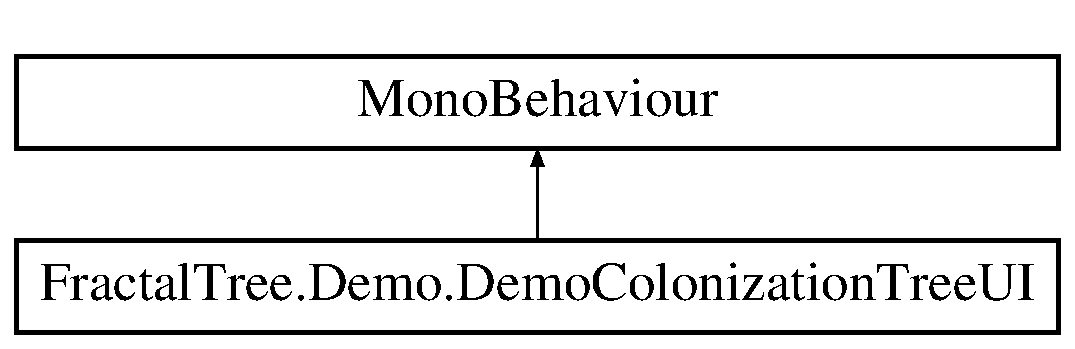
\includegraphics[height=2.000000cm]{class_fractal_tree_1_1_demo_1_1_demo_colonization_tree_u_i}
\end{center}
\end{figure}
\subsection*{Public Attributes}
\begin{DoxyCompactItemize}
\item 
\mbox{\Hypertarget{class_fractal_tree_1_1_demo_1_1_demo_colonization_tree_u_i_a1f35fb4533094cb2405feb983d4f0277}\label{class_fractal_tree_1_1_demo_1_1_demo_colonization_tree_u_i_a1f35fb4533094cb2405feb983d4f0277}} 
\hyperlink{class_fractal_tree_1_1_tree_builder}{Tree\+Builder} {\bfseries tree\+Builder}
\item 
\mbox{\Hypertarget{class_fractal_tree_1_1_demo_1_1_demo_colonization_tree_u_i_a2da328bf5dabb27257f3572b6a88a801}\label{class_fractal_tree_1_1_demo_1_1_demo_colonization_tree_u_i_a2da328bf5dabb27257f3572b6a88a801}} 
\hyperlink{class_fractal_tree_1_1_demo_leaf_placement}{Demo\+Leaf\+Placement} {\bfseries leaf\+Placement}
\item 
\mbox{\Hypertarget{class_fractal_tree_1_1_demo_1_1_demo_colonization_tree_u_i_a28700a0fa2b1d51bbba9f78963df211a}\label{class_fractal_tree_1_1_demo_1_1_demo_colonization_tree_u_i_a28700a0fa2b1d51bbba9f78963df211a}} 
Input\+Field {\bfseries length\+Input}
\item 
\mbox{\Hypertarget{class_fractal_tree_1_1_demo_1_1_demo_colonization_tree_u_i_a2fb1bc5036b68460bdf94fc5389492bf}\label{class_fractal_tree_1_1_demo_1_1_demo_colonization_tree_u_i_a2fb1bc5036b68460bdf94fc5389492bf}} 
Input\+Field {\bfseries width\+Input}
\item 
\mbox{\Hypertarget{class_fractal_tree_1_1_demo_1_1_demo_colonization_tree_u_i_adcb2fbc464c2484fa0e907632f8cd982}\label{class_fractal_tree_1_1_demo_1_1_demo_colonization_tree_u_i_adcb2fbc464c2484fa0e907632f8cd982}} 
Input\+Field {\bfseries min\+Distance\+To\+Leaf\+Input}
\item 
\mbox{\Hypertarget{class_fractal_tree_1_1_demo_1_1_demo_colonization_tree_u_i_a796c6ba7c169dab5f3ea3ae0b2be537c}\label{class_fractal_tree_1_1_demo_1_1_demo_colonization_tree_u_i_a796c6ba7c169dab5f3ea3ae0b2be537c}} 
Input\+Field {\bfseries max\+Distance\+To\+Leaf\+Input}
\item 
\mbox{\Hypertarget{class_fractal_tree_1_1_demo_1_1_demo_colonization_tree_u_i_abad44ab72a6599b2d195cae9f819eb92}\label{class_fractal_tree_1_1_demo_1_1_demo_colonization_tree_u_i_abad44ab72a6599b2d195cae9f819eb92}} 
Button {\bfseries clear\+Button}
\item 
\mbox{\Hypertarget{class_fractal_tree_1_1_demo_1_1_demo_colonization_tree_u_i_af43f21bb3bb65f680710b5e4555438c7}\label{class_fractal_tree_1_1_demo_1_1_demo_colonization_tree_u_i_af43f21bb3bb65f680710b5e4555438c7}} 
Button {\bfseries generate\+Button}
\end{DoxyCompactItemize}


\subsection{Detailed Description}
For demo purposes. Listens for changes in UI and updates Space Colonization variables. 



The documentation for this class was generated from the following file\+:\begin{DoxyCompactItemize}
\item 
F\+T/\+Scripts/\+Demo/Demo\+Colonization\+Tree\+U\+I.\+cs\end{DoxyCompactItemize}

\hypertarget{class_fractal_tree_1_1_demo_1_1_demo_controls}{}\section{Fractal\+Tree.\+Demo.\+Demo\+Controls Class Reference}
\label{class_fractal_tree_1_1_demo_1_1_demo_controls}\index{Fractal\+Tree.\+Demo.\+Demo\+Controls@{Fractal\+Tree.\+Demo.\+Demo\+Controls}}
Inheritance diagram for Fractal\+Tree.\+Demo.\+Demo\+Controls\+:\begin{figure}[H]
\begin{center}
\leavevmode
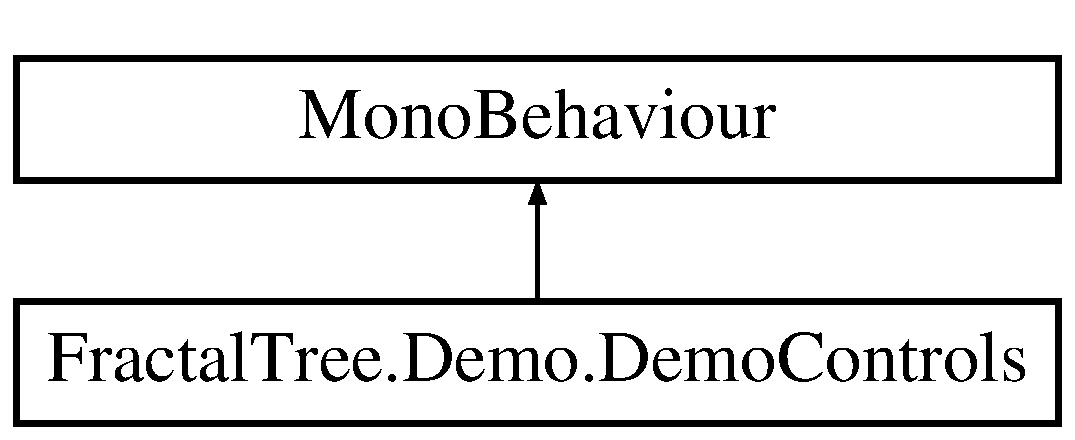
\includegraphics[height=2.000000cm]{class_fractal_tree_1_1_demo_1_1_demo_controls}
\end{center}
\end{figure}
\subsection*{Public Member Functions}
\begin{DoxyCompactItemize}
\item 
\mbox{\Hypertarget{class_fractal_tree_1_1_demo_1_1_demo_controls_a31ca5dcb7e12cf797ec714b78cedd5ef}\label{class_fractal_tree_1_1_demo_1_1_demo_controls_a31ca5dcb7e12cf797ec714b78cedd5ef}} 
void {\bfseries On\+Radius\+Changed} (string value)
\item 
\mbox{\Hypertarget{class_fractal_tree_1_1_demo_1_1_demo_controls_a2b7d31163419af37fb963c3391e96311}\label{class_fractal_tree_1_1_demo_1_1_demo_controls_a2b7d31163419af37fb963c3391e96311}} 
void {\bfseries On\+Push\+Changed} (string value)
\item 
\mbox{\Hypertarget{class_fractal_tree_1_1_demo_1_1_demo_controls_ab58233bc200b04f1c3862fae7bd6181f}\label{class_fractal_tree_1_1_demo_1_1_demo_controls_ab58233bc200b04f1c3862fae7bd6181f}} 
void {\bfseries On\+Pull\+Changed} (string value)
\item 
\mbox{\Hypertarget{class_fractal_tree_1_1_demo_1_1_demo_controls_a626d1d5b1c433eccc4fcddaae5b693ae}\label{class_fractal_tree_1_1_demo_1_1_demo_controls_a626d1d5b1c433eccc4fcddaae5b693ae}} 
void {\bfseries On\+Next\+Tree\+Pressed} ()
\item 
\mbox{\Hypertarget{class_fractal_tree_1_1_demo_1_1_demo_controls_a109d0a017190c30774b0d920edf85d0d}\label{class_fractal_tree_1_1_demo_1_1_demo_controls_a109d0a017190c30774b0d920edf85d0d}} 
void {\bfseries On\+Change\+Tree\+State\+Pressed} ()
\end{DoxyCompactItemize}
\subsection*{Public Attributes}
\begin{DoxyCompactItemize}
\item 
\mbox{\Hypertarget{class_fractal_tree_1_1_demo_1_1_demo_controls_ad8346155d93e759338a769ced6e17fda}\label{class_fractal_tree_1_1_demo_1_1_demo_controls_ad8346155d93e759338a769ced6e17fda}} 
Game\+Object {\bfseries controls}
\item 
\mbox{\Hypertarget{class_fractal_tree_1_1_demo_1_1_demo_controls_ab8bb391b544276436e84a06c4af69295}\label{class_fractal_tree_1_1_demo_1_1_demo_controls_ab8bb391b544276436e84a06c4af69295}} 
\hyperlink{class_fractal_tree_1_1_demo_1_1_demo_force_controller}{Demo\+Force\+Controller} {\bfseries force\+Controller}
\item 
\mbox{\Hypertarget{class_fractal_tree_1_1_demo_1_1_demo_controls_a8ebe734c3cfcbe467e22173777825f6b}\label{class_fractal_tree_1_1_demo_1_1_demo_controls_a8ebe734c3cfcbe467e22173777825f6b}} 
\hyperlink{class_fractal_tree_1_1_demo_1_1_demo_tree_creator}{Demo\+Tree\+Creator} {\bfseries tree\+Creator}
\item 
\mbox{\Hypertarget{class_fractal_tree_1_1_demo_1_1_demo_controls_a368597dd8008c3cc8cc7a5c336b44faa}\label{class_fractal_tree_1_1_demo_1_1_demo_controls_a368597dd8008c3cc8cc7a5c336b44faa}} 
Input\+Field {\bfseries radius\+Input}
\item 
\mbox{\Hypertarget{class_fractal_tree_1_1_demo_1_1_demo_controls_af9fa15fa4782f33b17a87eb230ec7dc1}\label{class_fractal_tree_1_1_demo_1_1_demo_controls_af9fa15fa4782f33b17a87eb230ec7dc1}} 
Input\+Field {\bfseries push\+Input}
\item 
\mbox{\Hypertarget{class_fractal_tree_1_1_demo_1_1_demo_controls_ae1abb5ada8caf9f44f7945f9bfad91d5}\label{class_fractal_tree_1_1_demo_1_1_demo_controls_ae1abb5ada8caf9f44f7945f9bfad91d5}} 
Input\+Field {\bfseries pull\+Input}
\item 
\mbox{\Hypertarget{class_fractal_tree_1_1_demo_1_1_demo_controls_ad2fdbc4da61fcb459f58a11eaf51157c}\label{class_fractal_tree_1_1_demo_1_1_demo_controls_ad2fdbc4da61fcb459f58a11eaf51157c}} 
Text {\bfseries stationary\+Button\+Text}
\item 
\mbox{\Hypertarget{class_fractal_tree_1_1_demo_1_1_demo_controls_a69bea268d002e8fc8c3dc23770bbbbe6}\label{class_fractal_tree_1_1_demo_1_1_demo_controls_a69bea268d002e8fc8c3dc23770bbbbe6}} 
Text {\bfseries warning\+Label}
\end{DoxyCompactItemize}


The documentation for this class was generated from the following file\+:\begin{DoxyCompactItemize}
\item 
F\+T/\+Scripts/\+Demo/Demo\+Controls.\+cs\end{DoxyCompactItemize}

\hypertarget{class_fractal_tree_1_1_demo_1_1_demo_force_controller}{}\section{Fractal\+Tree.\+Demo.\+Demo\+Force\+Controller Class Reference}
\label{class_fractal_tree_1_1_demo_1_1_demo_force_controller}\index{Fractal\+Tree.\+Demo.\+Demo\+Force\+Controller@{Fractal\+Tree.\+Demo.\+Demo\+Force\+Controller}}


Applies forces to the currently active tree in the demo scene.  


Inheritance diagram for Fractal\+Tree.\+Demo.\+Demo\+Force\+Controller\+:\begin{figure}[H]
\begin{center}
\leavevmode
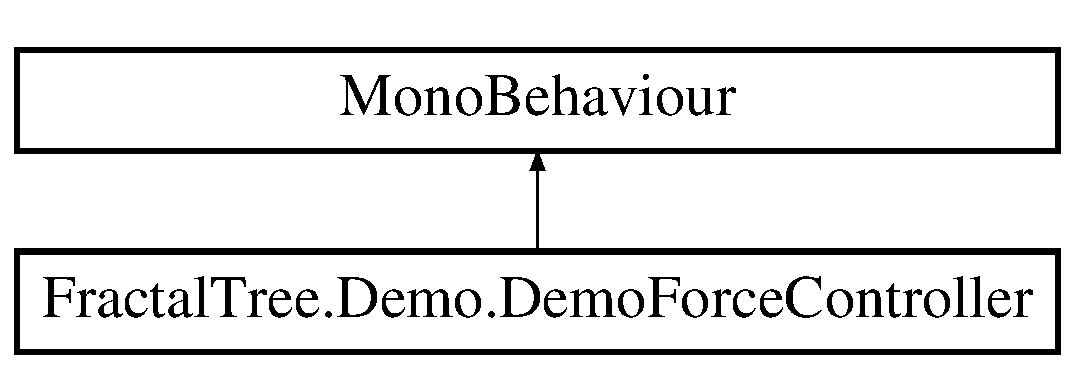
\includegraphics[height=2.000000cm]{class_fractal_tree_1_1_demo_1_1_demo_force_controller}
\end{center}
\end{figure}
\subsection*{Public Attributes}
\begin{DoxyCompactItemize}
\item 
\mbox{\Hypertarget{class_fractal_tree_1_1_demo_1_1_demo_force_controller_ab3ad5eba7a7a4f2d74e543572e2eb052}\label{class_fractal_tree_1_1_demo_1_1_demo_force_controller_ab3ad5eba7a7a4f2d74e543572e2eb052}} 
\hyperlink{class_fractal_tree_1_1_demo_1_1_demo_tree_creator}{Demo\+Tree\+Creator} {\bfseries tree\+Creator}
\item 
\mbox{\Hypertarget{class_fractal_tree_1_1_demo_1_1_demo_force_controller_ad23d270ac91d98230b4b99fe57a31c46}\label{class_fractal_tree_1_1_demo_1_1_demo_force_controller_ad23d270ac91d98230b4b99fe57a31c46}} 
float {\bfseries radius} = 10
\item 
\mbox{\Hypertarget{class_fractal_tree_1_1_demo_1_1_demo_force_controller_acc0f4abc1f05d8de48bf509c51bfd2c2}\label{class_fractal_tree_1_1_demo_1_1_demo_force_controller_acc0f4abc1f05d8de48bf509c51bfd2c2}} 
float {\bfseries push\+Force} = 2f
\item 
\mbox{\Hypertarget{class_fractal_tree_1_1_demo_1_1_demo_force_controller_a05e469959fcc15a37563169ed7d21723}\label{class_fractal_tree_1_1_demo_1_1_demo_force_controller_a05e469959fcc15a37563169ed7d21723}} 
float {\bfseries pull\+Force} = 0.\+1f
\item 
\mbox{\Hypertarget{class_fractal_tree_1_1_demo_1_1_demo_force_controller_aa6e3af65965f03534e7a0a112dbf9c15}\label{class_fractal_tree_1_1_demo_1_1_demo_force_controller_aa6e3af65965f03534e7a0a112dbf9c15}} 
float {\bfseries directed\+Force} = 0.\+5f
\end{DoxyCompactItemize}


\subsection{Detailed Description}
Applies forces to the currently active tree in the demo scene. 



The documentation for this class was generated from the following file\+:\begin{DoxyCompactItemize}
\item 
F\+T/\+Scripts/\+Demo/Demo\+Force\+Controller.\+cs\end{DoxyCompactItemize}

\hypertarget{class_fractal_tree_1_1_demo_leaf_placement}{}\section{Fractal\+Tree.\+Demo\+Leaf\+Placement Class Reference}
\label{class_fractal_tree_1_1_demo_leaf_placement}\index{Fractal\+Tree.\+Demo\+Leaf\+Placement@{Fractal\+Tree.\+Demo\+Leaf\+Placement}}


For demo purposes. Spawns a leaf object (used for space colonization tree algorithm) at mouse position on left-\/click.  


Inheritance diagram for Fractal\+Tree.\+Demo\+Leaf\+Placement\+:\begin{figure}[H]
\begin{center}
\leavevmode
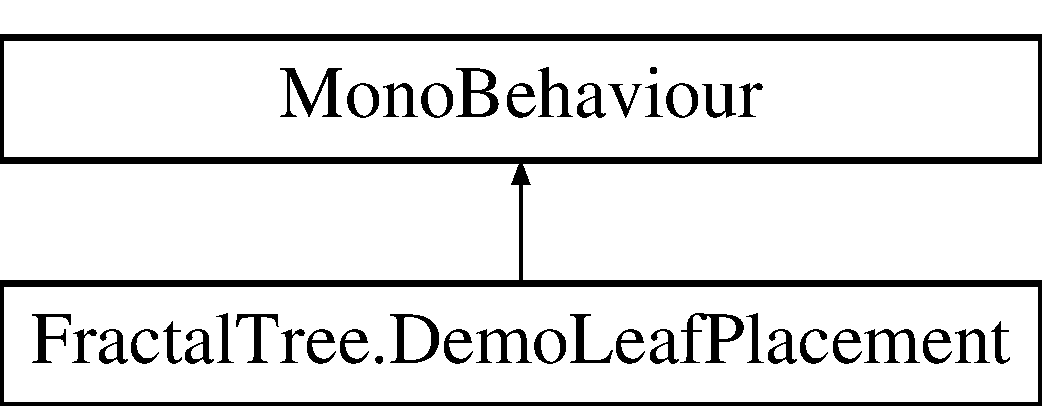
\includegraphics[height=2.000000cm]{class_fractal_tree_1_1_demo_leaf_placement}
\end{center}
\end{figure}
\subsection*{Public Member Functions}
\begin{DoxyCompactItemize}
\item 
void \hyperlink{class_fractal_tree_1_1_demo_leaf_placement_a745d74525906a3177b7ac67ac94280cf}{Clear} ()
\begin{DoxyCompactList}\small\item\em Remove all child leaves. \end{DoxyCompactList}\end{DoxyCompactItemize}
\subsection*{Public Attributes}
\begin{DoxyCompactItemize}
\item 
\mbox{\Hypertarget{class_fractal_tree_1_1_demo_leaf_placement_ad416455c3c21399f1b5cf36dd70ed60b}\label{class_fractal_tree_1_1_demo_leaf_placement_ad416455c3c21399f1b5cf36dd70ed60b}} 
Game\+Object {\bfseries leaf\+Prefab}
\end{DoxyCompactItemize}


\subsection{Detailed Description}
For demo purposes. Spawns a leaf object (used for space colonization tree algorithm) at mouse position on left-\/click. 



\subsection{Member Function Documentation}
\mbox{\Hypertarget{class_fractal_tree_1_1_demo_leaf_placement_a745d74525906a3177b7ac67ac94280cf}\label{class_fractal_tree_1_1_demo_leaf_placement_a745d74525906a3177b7ac67ac94280cf}} 
\index{Fractal\+Tree\+::\+Demo\+Leaf\+Placement@{Fractal\+Tree\+::\+Demo\+Leaf\+Placement}!Clear@{Clear}}
\index{Clear@{Clear}!Fractal\+Tree\+::\+Demo\+Leaf\+Placement@{Fractal\+Tree\+::\+Demo\+Leaf\+Placement}}
\subsubsection{\texorpdfstring{Clear()}{Clear()}}
{\footnotesize\ttfamily void Fractal\+Tree.\+Demo\+Leaf\+Placement.\+Clear (\begin{DoxyParamCaption}{ }\end{DoxyParamCaption})}



Remove all child leaves. 



The documentation for this class was generated from the following file\+:\begin{DoxyCompactItemize}
\item 
F\+T/\+Scripts/\+Demo/Demo\+Leaf\+Placement.\+cs\end{DoxyCompactItemize}

\hypertarget{class_fractal_tree_1_1_demo_1_1_demo_l_tree_u_i}{}\section{Fractal\+Tree.\+Demo.\+Demo\+L\+Tree\+UI Class Reference}
\label{class_fractal_tree_1_1_demo_1_1_demo_l_tree_u_i}\index{Fractal\+Tree.\+Demo.\+Demo\+L\+Tree\+UI@{Fractal\+Tree.\+Demo.\+Demo\+L\+Tree\+UI}}


For demo purposes. Listens for changes in UI and updates L-\/\+Tree variables.  


Inheritance diagram for Fractal\+Tree.\+Demo.\+Demo\+L\+Tree\+UI\+:\begin{figure}[H]
\begin{center}
\leavevmode
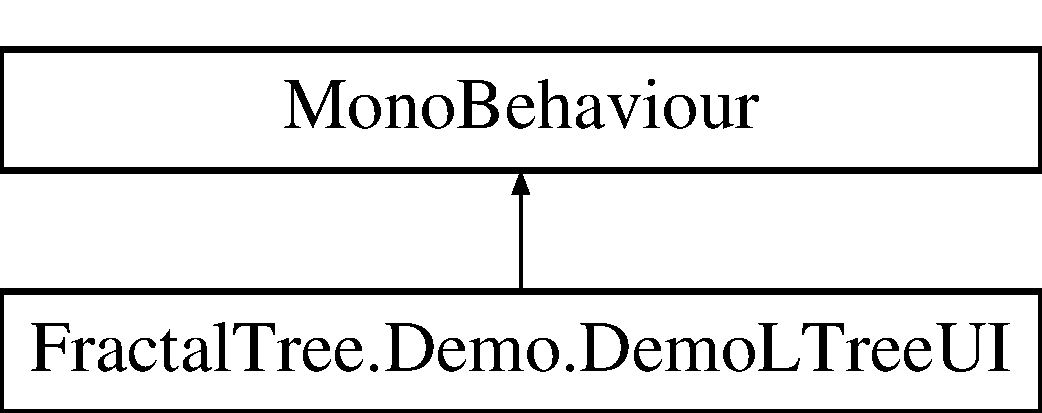
\includegraphics[height=2.000000cm]{class_fractal_tree_1_1_demo_1_1_demo_l_tree_u_i}
\end{center}
\end{figure}
\subsection*{Public Attributes}
\begin{DoxyCompactItemize}
\item 
\mbox{\Hypertarget{class_fractal_tree_1_1_demo_1_1_demo_l_tree_u_i_a29954afb766fe5ef22708acfed0406be}\label{class_fractal_tree_1_1_demo_1_1_demo_l_tree_u_i_a29954afb766fe5ef22708acfed0406be}} 
\hyperlink{class_fractal_tree_1_1_tree_builder}{Tree\+Builder} {\bfseries tree\+Builder}
\item 
\mbox{\Hypertarget{class_fractal_tree_1_1_demo_1_1_demo_l_tree_u_i_a35095cdc2d943f10eebf668a8c89792f}\label{class_fractal_tree_1_1_demo_1_1_demo_l_tree_u_i_a35095cdc2d943f10eebf668a8c89792f}} 
Toggle {\bfseries auto\+Width\+Toggle}
\item 
\mbox{\Hypertarget{class_fractal_tree_1_1_demo_1_1_demo_l_tree_u_i_a8337c29e68c73a086eeff4fd5ceb678e}\label{class_fractal_tree_1_1_demo_1_1_demo_l_tree_u_i_a8337c29e68c73a086eeff4fd5ceb678e}} 
Input\+Field {\bfseries width\+Input}
\item 
\mbox{\Hypertarget{class_fractal_tree_1_1_demo_1_1_demo_l_tree_u_i_aab8a985a8a1f32dab8ba8a764d4b1456}\label{class_fractal_tree_1_1_demo_1_1_demo_l_tree_u_i_aab8a985a8a1f32dab8ba8a764d4b1456}} 
Input\+Field {\bfseries gen\+Input}
\item 
\mbox{\Hypertarget{class_fractal_tree_1_1_demo_1_1_demo_l_tree_u_i_afdb15881135d26460fe1312aa42df550}\label{class_fractal_tree_1_1_demo_1_1_demo_l_tree_u_i_afdb15881135d26460fe1312aa42df550}} 
Input\+Field {\bfseries length\+Input}
\item 
\mbox{\Hypertarget{class_fractal_tree_1_1_demo_1_1_demo_l_tree_u_i_af3631be21ca9d41a4bbdf969f04a458c}\label{class_fractal_tree_1_1_demo_1_1_demo_l_tree_u_i_af3631be21ca9d41a4bbdf969f04a458c}} 
Input\+Field {\bfseries angle\+Input}
\item 
\mbox{\Hypertarget{class_fractal_tree_1_1_demo_1_1_demo_l_tree_u_i_af6fcf8dae21063a705eac204483d0208}\label{class_fractal_tree_1_1_demo_1_1_demo_l_tree_u_i_af6fcf8dae21063a705eac204483d0208}} 
Input\+Field {\bfseries axiom\+Input}
\item 
\mbox{\Hypertarget{class_fractal_tree_1_1_demo_1_1_demo_l_tree_u_i_a27f93ea90e35205c11a963d68f7696d6}\label{class_fractal_tree_1_1_demo_1_1_demo_l_tree_u_i_a27f93ea90e35205c11a963d68f7696d6}} 
Input\+Field \mbox{[}$\,$\mbox{]} {\bfseries rule\+Inputs}
\item 
\mbox{\Hypertarget{class_fractal_tree_1_1_demo_1_1_demo_l_tree_u_i_a0c71d7d0387e939fb5fa7ad9db2dae2c}\label{class_fractal_tree_1_1_demo_1_1_demo_l_tree_u_i_a0c71d7d0387e939fb5fa7ad9db2dae2c}} 
Button {\bfseries generate}
\end{DoxyCompactItemize}


\subsection{Detailed Description}
For demo purposes. Listens for changes in UI and updates L-\/\+Tree variables. 



The documentation for this class was generated from the following file\+:\begin{DoxyCompactItemize}
\item 
F\+T/\+Scripts/\+Demo/Demo\+L\+Tree\+U\+I.\+cs\end{DoxyCompactItemize}

\hypertarget{class_fractal_tree_1_1_demo_1_1_demo_scene_switcher}{}\section{Fractal\+Tree.\+Demo.\+Demo\+Scene\+Switcher Class Reference}
\label{class_fractal_tree_1_1_demo_1_1_demo_scene_switcher}\index{Fractal\+Tree.\+Demo.\+Demo\+Scene\+Switcher@{Fractal\+Tree.\+Demo.\+Demo\+Scene\+Switcher}}
Inheritance diagram for Fractal\+Tree.\+Demo.\+Demo\+Scene\+Switcher\+:\begin{figure}[H]
\begin{center}
\leavevmode
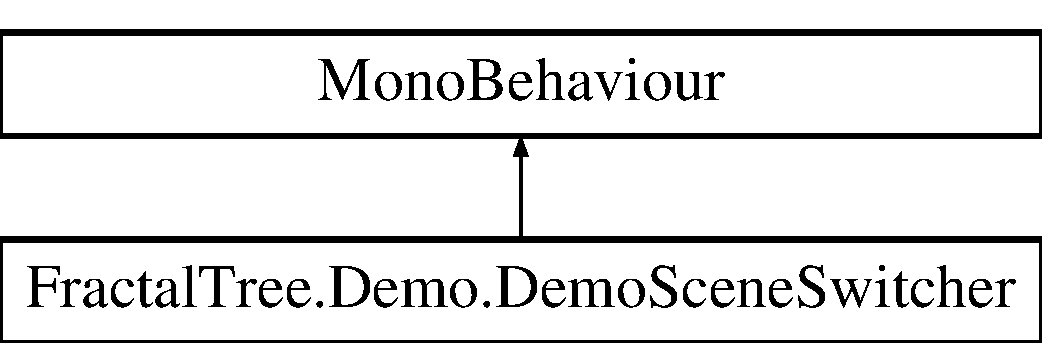
\includegraphics[height=2.000000cm]{class_fractal_tree_1_1_demo_1_1_demo_scene_switcher}
\end{center}
\end{figure}
\subsection*{Public Member Functions}
\begin{DoxyCompactItemize}
\item 
\mbox{\Hypertarget{class_fractal_tree_1_1_demo_1_1_demo_scene_switcher_a2c4499cd9b20b5be784aea61d3ff4cd4}\label{class_fractal_tree_1_1_demo_1_1_demo_scene_switcher_a2c4499cd9b20b5be784aea61d3ff4cd4}} 
void {\bfseries Load\+Next\+Scene} ()
\end{DoxyCompactItemize}
\subsection*{Public Attributes}
\begin{DoxyCompactItemize}
\item 
\mbox{\Hypertarget{class_fractal_tree_1_1_demo_1_1_demo_scene_switcher_a6393450e105e7e68ff2dc67942140593}\label{class_fractal_tree_1_1_demo_1_1_demo_scene_switcher_a6393450e105e7e68ff2dc67942140593}} 
int {\bfseries num\+Of\+Scenes} = 2
\end{DoxyCompactItemize}


The documentation for this class was generated from the following file\+:\begin{DoxyCompactItemize}
\item 
F\+T/\+Scripts/\+Demo/Demo\+Scene\+Switcher.\+cs\end{DoxyCompactItemize}

\hypertarget{class_fractal_tree_1_1_demo_1_1_demo_tree_creator}{}\section{Fractal\+Tree.\+Demo.\+Demo\+Tree\+Creator Class Reference}
\label{class_fractal_tree_1_1_demo_1_1_demo_tree_creator}\index{Fractal\+Tree.\+Demo.\+Demo\+Tree\+Creator@{Fractal\+Tree.\+Demo.\+Demo\+Tree\+Creator}}
Inheritance diagram for Fractal\+Tree.\+Demo.\+Demo\+Tree\+Creator\+:\begin{figure}[H]
\begin{center}
\leavevmode
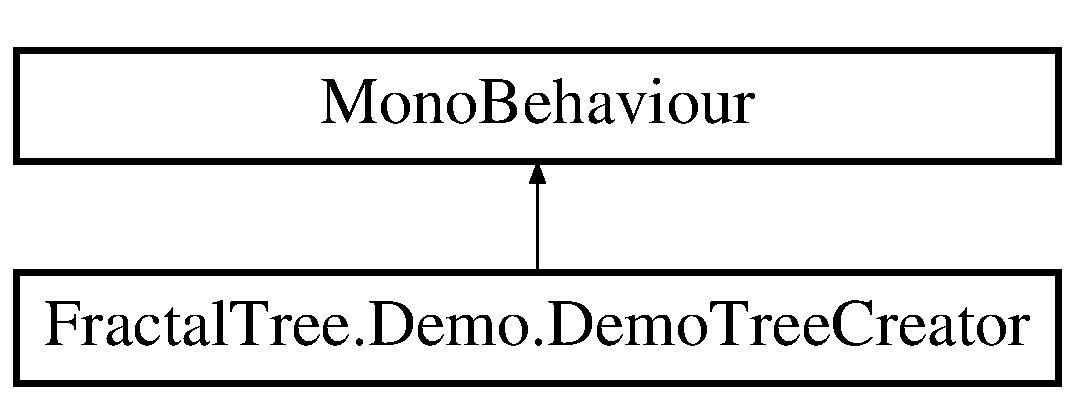
\includegraphics[height=2.000000cm]{class_fractal_tree_1_1_demo_1_1_demo_tree_creator}
\end{center}
\end{figure}
\subsection*{Public Member Functions}
\begin{DoxyCompactItemize}
\item 
\mbox{\Hypertarget{class_fractal_tree_1_1_demo_1_1_demo_tree_creator_a6bacdd305fc4484980730e71d22d8c37}\label{class_fractal_tree_1_1_demo_1_1_demo_tree_creator_a6bacdd305fc4484980730e71d22d8c37}} 
void {\bfseries Show\+Next\+Tree} ()
\item 
\mbox{\Hypertarget{class_fractal_tree_1_1_demo_1_1_demo_tree_creator_a82a2a0699f5bb6e0af8228d98672cf5f}\label{class_fractal_tree_1_1_demo_1_1_demo_tree_creator_a82a2a0699f5bb6e0af8228d98672cf5f}} 
bool {\bfseries Switch\+Tree\+State} ()
\end{DoxyCompactItemize}
\subsection*{Public Attributes}
\begin{DoxyCompactItemize}
\item 
\hyperlink{class_fractal_tree_1_1_demo_1_1_trees_to_demo}{Trees\+To\+Demo} \mbox{[}$\,$\mbox{]} \hyperlink{class_fractal_tree_1_1_demo_1_1_demo_tree_creator_a467fca64d8fc1098bc4684bd9987850c}{tree\+Builders}
\begin{DoxyCompactList}\small\item\em A list of stationary and moving tree pairs with helper methods to switch between them. \end{DoxyCompactList}\item 
\hyperlink{class_fractal_tree_1_1_colonization_leaf_generator}{Colonization\+Leaf\+Generator} \hyperlink{class_fractal_tree_1_1_demo_1_1_demo_tree_creator_aa359c2bdf8c008848518f4c67cb5df53}{leaf\+Generator}
\begin{DoxyCompactList}\small\item\em A leaf generator used for space colonization trees. \end{DoxyCompactList}\item 
bool \hyperlink{class_fractal_tree_1_1_demo_1_1_demo_tree_creator_a17a43b81fc0033481925e700fc2011f4}{showing\+Stationary} = true
\begin{DoxyCompactList}\small\item\em Showing a static or moving version of the tree. \end{DoxyCompactList}\item 
\mbox{\Hypertarget{class_fractal_tree_1_1_demo_1_1_demo_tree_creator_afcb3eaaf09e36ee8030025eca5d31888}\label{class_fractal_tree_1_1_demo_1_1_demo_tree_creator_afcb3eaaf09e36ee8030025eca5d31888}} 
int {\bfseries start\+Index} = 0
\end{DoxyCompactItemize}
\subsection*{Properties}
\begin{DoxyCompactItemize}
\item 
\hyperlink{class_fractal_tree_1_1_tree_builder}{Tree\+Builder} \hyperlink{class_fractal_tree_1_1_demo_1_1_demo_tree_creator_a67e1b37c9ecc60e628533b069c3c0d98}{active\+Tree}\hspace{0.3cm}{\ttfamily  \mbox{[}get\mbox{]}}
\begin{DoxyCompactList}\small\item\em Gets the active tree or null if there is none. \end{DoxyCompactList}\end{DoxyCompactItemize}


\subsection{Member Data Documentation}
\mbox{\Hypertarget{class_fractal_tree_1_1_demo_1_1_demo_tree_creator_aa359c2bdf8c008848518f4c67cb5df53}\label{class_fractal_tree_1_1_demo_1_1_demo_tree_creator_aa359c2bdf8c008848518f4c67cb5df53}} 
\index{Fractal\+Tree\+::\+Demo\+::\+Demo\+Tree\+Creator@{Fractal\+Tree\+::\+Demo\+::\+Demo\+Tree\+Creator}!leaf\+Generator@{leaf\+Generator}}
\index{leaf\+Generator@{leaf\+Generator}!Fractal\+Tree\+::\+Demo\+::\+Demo\+Tree\+Creator@{Fractal\+Tree\+::\+Demo\+::\+Demo\+Tree\+Creator}}
\subsubsection{\texorpdfstring{leaf\+Generator}{leafGenerator}}
{\footnotesize\ttfamily \hyperlink{class_fractal_tree_1_1_colonization_leaf_generator}{Colonization\+Leaf\+Generator} Fractal\+Tree.\+Demo.\+Demo\+Tree\+Creator.\+leaf\+Generator}



A leaf generator used for space colonization trees. 

\mbox{\Hypertarget{class_fractal_tree_1_1_demo_1_1_demo_tree_creator_a17a43b81fc0033481925e700fc2011f4}\label{class_fractal_tree_1_1_demo_1_1_demo_tree_creator_a17a43b81fc0033481925e700fc2011f4}} 
\index{Fractal\+Tree\+::\+Demo\+::\+Demo\+Tree\+Creator@{Fractal\+Tree\+::\+Demo\+::\+Demo\+Tree\+Creator}!showing\+Stationary@{showing\+Stationary}}
\index{showing\+Stationary@{showing\+Stationary}!Fractal\+Tree\+::\+Demo\+::\+Demo\+Tree\+Creator@{Fractal\+Tree\+::\+Demo\+::\+Demo\+Tree\+Creator}}
\subsubsection{\texorpdfstring{showing\+Stationary}{showingStationary}}
{\footnotesize\ttfamily bool Fractal\+Tree.\+Demo.\+Demo\+Tree\+Creator.\+showing\+Stationary = true}



Showing a static or moving version of the tree. 

\mbox{\Hypertarget{class_fractal_tree_1_1_demo_1_1_demo_tree_creator_a467fca64d8fc1098bc4684bd9987850c}\label{class_fractal_tree_1_1_demo_1_1_demo_tree_creator_a467fca64d8fc1098bc4684bd9987850c}} 
\index{Fractal\+Tree\+::\+Demo\+::\+Demo\+Tree\+Creator@{Fractal\+Tree\+::\+Demo\+::\+Demo\+Tree\+Creator}!tree\+Builders@{tree\+Builders}}
\index{tree\+Builders@{tree\+Builders}!Fractal\+Tree\+::\+Demo\+::\+Demo\+Tree\+Creator@{Fractal\+Tree\+::\+Demo\+::\+Demo\+Tree\+Creator}}
\subsubsection{\texorpdfstring{tree\+Builders}{treeBuilders}}
{\footnotesize\ttfamily \hyperlink{class_fractal_tree_1_1_demo_1_1_trees_to_demo}{Trees\+To\+Demo} \mbox{[}$\,$\mbox{]} Fractal\+Tree.\+Demo.\+Demo\+Tree\+Creator.\+tree\+Builders}



A list of stationary and moving tree pairs with helper methods to switch between them. 



\subsection{Property Documentation}
\mbox{\Hypertarget{class_fractal_tree_1_1_demo_1_1_demo_tree_creator_a67e1b37c9ecc60e628533b069c3c0d98}\label{class_fractal_tree_1_1_demo_1_1_demo_tree_creator_a67e1b37c9ecc60e628533b069c3c0d98}} 
\index{Fractal\+Tree\+::\+Demo\+::\+Demo\+Tree\+Creator@{Fractal\+Tree\+::\+Demo\+::\+Demo\+Tree\+Creator}!active\+Tree@{active\+Tree}}
\index{active\+Tree@{active\+Tree}!Fractal\+Tree\+::\+Demo\+::\+Demo\+Tree\+Creator@{Fractal\+Tree\+::\+Demo\+::\+Demo\+Tree\+Creator}}
\subsubsection{\texorpdfstring{active\+Tree}{activeTree}}
{\footnotesize\ttfamily \hyperlink{class_fractal_tree_1_1_tree_builder}{Tree\+Builder} Fractal\+Tree.\+Demo.\+Demo\+Tree\+Creator.\+active\+Tree\hspace{0.3cm}{\ttfamily [get]}}



Gets the active tree or null if there is none. 

The active tree.

The documentation for this class was generated from the following file\+:\begin{DoxyCompactItemize}
\item 
F\+T/\+Scripts/\+Demo/Demo\+Tree\+Creator.\+cs\end{DoxyCompactItemize}

\hypertarget{class_fractal_tree_1_1_demo_1_1_demo_tree_data}{}\section{Fractal\+Tree.\+Demo.\+Demo\+Tree\+Data Class Reference}
\label{class_fractal_tree_1_1_demo_1_1_demo_tree_data}\index{Fractal\+Tree.\+Demo.\+Demo\+Tree\+Data@{Fractal\+Tree.\+Demo.\+Demo\+Tree\+Data}}
Inheritance diagram for Fractal\+Tree.\+Demo.\+Demo\+Tree\+Data\+:\begin{figure}[H]
\begin{center}
\leavevmode
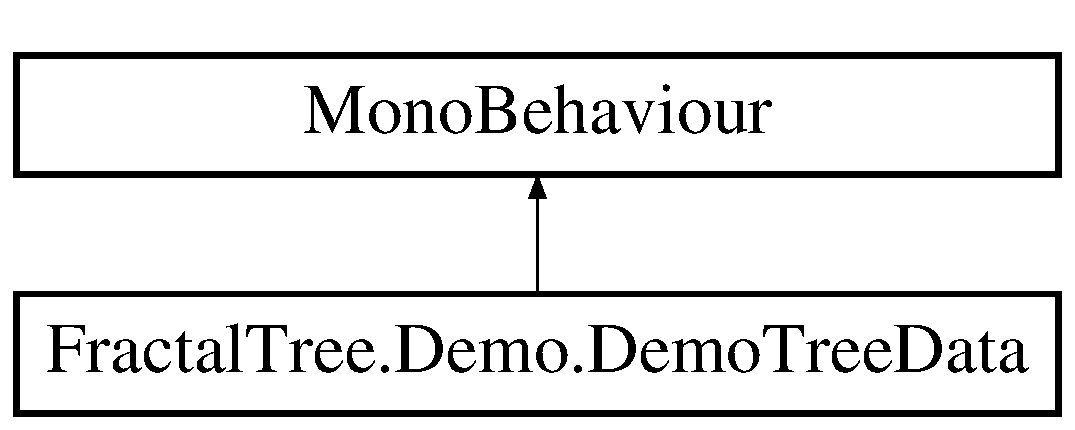
\includegraphics[height=2.000000cm]{class_fractal_tree_1_1_demo_1_1_demo_tree_data}
\end{center}
\end{figure}
\subsection*{Public Attributes}
\begin{DoxyCompactItemize}
\item 
\mbox{\Hypertarget{class_fractal_tree_1_1_demo_1_1_demo_tree_data_a2d91fd17585a79e5389e4b30e12fa9fc}\label{class_fractal_tree_1_1_demo_1_1_demo_tree_data_a2d91fd17585a79e5389e4b30e12fa9fc}} 
\hyperlink{class_fractal_tree_1_1_demo_1_1_demo_tree_creator}{Demo\+Tree\+Creator} {\bfseries tree\+Creator}
\end{DoxyCompactItemize}


The documentation for this class was generated from the following file\+:\begin{DoxyCompactItemize}
\item 
F\+T/\+Scripts/\+Demo/Demo\+Tree\+Data.\+cs\end{DoxyCompactItemize}

\hypertarget{class_fractal_tree_1_1_l_rule}{}\section{Fractal\+Tree.\+L\+Rule Class Reference}
\label{class_fractal_tree_1_1_l_rule}\index{Fractal\+Tree.\+L\+Rule@{Fractal\+Tree.\+L\+Rule}}
\subsection*{Public Member Functions}
\begin{DoxyCompactItemize}
\item 
\hypertarget{class_fractal_tree_1_1_l_rule_a35f380166641f36ee4290895cecc4583}{}\label{class_fractal_tree_1_1_l_rule_a35f380166641f36ee4290895cecc4583} 
{\bfseries L\+Rule} (char from, string to)
\end{DoxyCompactItemize}
\subsection*{Public Attributes}
\begin{DoxyCompactItemize}
\item 
\hypertarget{class_fractal_tree_1_1_l_rule_aa08500e91663051c5da038421de7a5d5}{}\label{class_fractal_tree_1_1_l_rule_aa08500e91663051c5da038421de7a5d5} 
char {\bfseries from}
\item 
\hypertarget{class_fractal_tree_1_1_l_rule_aaa28686eef06632f5c6b0d71ff7c615e}{}\label{class_fractal_tree_1_1_l_rule_aaa28686eef06632f5c6b0d71ff7c615e} 
string {\bfseries to}
\end{DoxyCompactItemize}


The documentation for this class was generated from the following file\+:\begin{DoxyCompactItemize}
\item 
L\+Tree.\+cs\end{DoxyCompactItemize}

\hypertarget{class_fractal_tree_1_1_l_tree}{}\section{Fractal\+Tree.\+L\+Tree Class Reference}
\label{class_fractal_tree_1_1_l_tree}\index{Fractal\+Tree.\+L\+Tree@{Fractal\+Tree.\+L\+Tree}}


Spawns a fractal true using the L-\/system\+: \href{http://www.allenpike.com/modeling-plants-with-l-systems/}{\tt http\+://www.\+allenpike.\+com/modeling-\/plants-\/with-\/l-\/systems/}  


Inheritance diagram for Fractal\+Tree.\+L\+Tree\+:\begin{figure}[H]
\begin{center}
\leavevmode
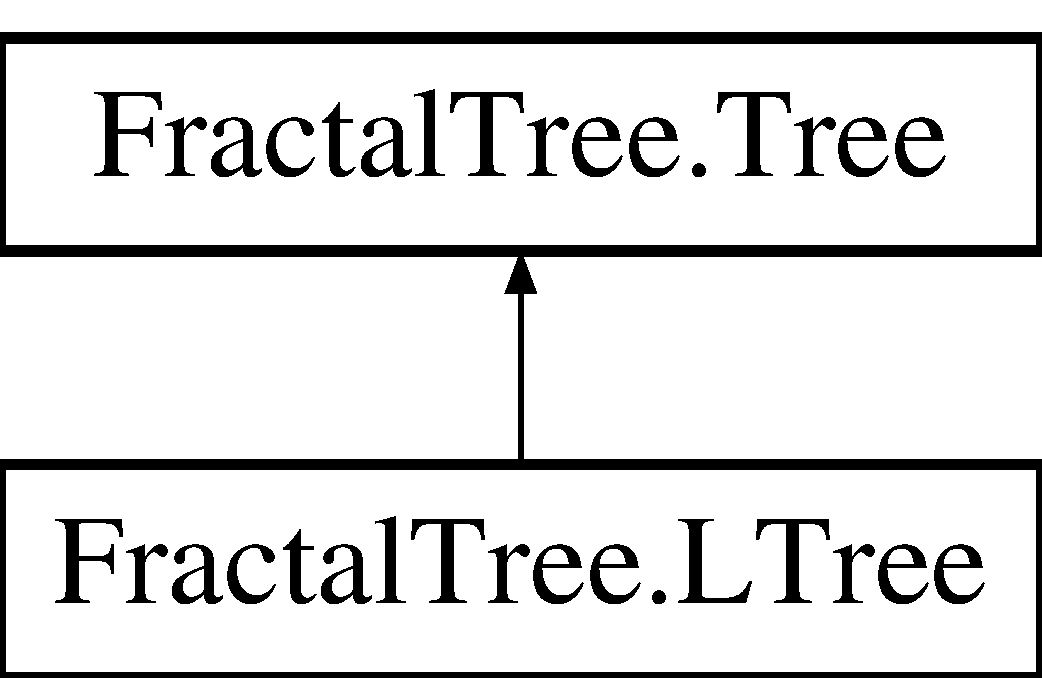
\includegraphics[height=2.000000cm]{class_fractal_tree_1_1_l_tree}
\end{center}
\end{figure}
\subsection*{Public Member Functions}
\begin{DoxyCompactItemize}
\item 
\hyperlink{class_fractal_tree_1_1_l_tree_aac93139ff0e0b365ca88c2ff38ae1595}{L\+Tree} (Game\+Object branch\+Prefab, int steps, string axiom, \hyperlink{class_fractal_tree_1_1_l_rule}{L\+Rule}\mbox{[}$\,$\mbox{]} rules, float branch\+Length, float angle, Transform owner, Color\mbox{[}$\,$\mbox{]} colors, float width, bool auto\+Width, bool auto\+Mass)
\begin{DoxyCompactList}\small\item\em Initializes a new instance of the \hyperlink{class_fractal_tree_1_1_l_tree}{Fractal\+Tree.\+L\+Tree} class. \end{DoxyCompactList}\item 
List$<$ T $>$ \hyperlink{class_fractal_tree_1_1_l_tree_a36b2a48dbb01982a649f8949823464fc}{Generate$<$ T $>$} ()
\begin{DoxyCompactList}\small\item\em Generates the tree. \end{DoxyCompactList}\end{DoxyCompactItemize}


\subsection{Detailed Description}
Spawns a fractal true using the L-\/system\+: \href{http://www.allenpike.com/modeling-plants-with-l-systems/}{\tt http\+://www.\+allenpike.\+com/modeling-\/plants-\/with-\/l-\/systems/} 



\subsection{Constructor \& Destructor Documentation}
\mbox{\Hypertarget{class_fractal_tree_1_1_l_tree_aac93139ff0e0b365ca88c2ff38ae1595}\label{class_fractal_tree_1_1_l_tree_aac93139ff0e0b365ca88c2ff38ae1595}} 
\index{Fractal\+Tree\+::\+L\+Tree@{Fractal\+Tree\+::\+L\+Tree}!L\+Tree@{L\+Tree}}
\index{L\+Tree@{L\+Tree}!Fractal\+Tree\+::\+L\+Tree@{Fractal\+Tree\+::\+L\+Tree}}
\subsubsection{\texorpdfstring{L\+Tree()}{LTree()}}
{\footnotesize\ttfamily Fractal\+Tree.\+L\+Tree.\+L\+Tree (\begin{DoxyParamCaption}\item[{Game\+Object}]{branch\+Prefab,  }\item[{int}]{steps,  }\item[{string}]{axiom,  }\item[{\hyperlink{class_fractal_tree_1_1_l_rule}{L\+Rule} \mbox{[}$\,$\mbox{]}}]{rules,  }\item[{float}]{branch\+Length,  }\item[{float}]{angle,  }\item[{Transform}]{owner,  }\item[{Color \mbox{[}$\,$\mbox{]}}]{colors,  }\item[{float}]{width,  }\item[{bool}]{auto\+Width,  }\item[{bool}]{auto\+Mass }\end{DoxyParamCaption})}



Initializes a new instance of the \hyperlink{class_fractal_tree_1_1_l_tree}{Fractal\+Tree.\+L\+Tree} class. 


\begin{DoxyParams}{Parameters}
{\em branch\+Prefab} & \hyperlink{interface_fractal_tree_1_1_branch}{Branch} prefab.\\
\hline
{\em steps} & Steps.\\
\hline
{\em axiom} & Axiom.\\
\hline
{\em rules} & Rules.\\
\hline
{\em initial\+Length} & Initial length.\\
\hline
{\em angle} & Angle.\\
\hline
{\em owner} & Owner.\\
\hline
{\em colors} & Colors.\\
\hline
{\em width} & Width.\\
\hline
{\em auto\+Width} & If set to {\ttfamily true} auto width.\\
\hline
{\em auto\+Mass} & If set to {\ttfamily true} auto mass.\\
\hline
\end{DoxyParams}


\subsection{Member Function Documentation}
\mbox{\Hypertarget{class_fractal_tree_1_1_l_tree_a36b2a48dbb01982a649f8949823464fc}\label{class_fractal_tree_1_1_l_tree_a36b2a48dbb01982a649f8949823464fc}} 
\index{Fractal\+Tree\+::\+L\+Tree@{Fractal\+Tree\+::\+L\+Tree}!Generate$<$ T $>$@{Generate$<$ T $>$}}
\index{Generate$<$ T $>$@{Generate$<$ T $>$}!Fractal\+Tree\+::\+L\+Tree@{Fractal\+Tree\+::\+L\+Tree}}
\subsubsection{\texorpdfstring{Generate$<$ T $>$()}{Generate< T >()}}
{\footnotesize\ttfamily List$<$T$>$ Fractal\+Tree.\+L\+Tree.\+Generate$<$ T $>$ (\begin{DoxyParamCaption}{ }\end{DoxyParamCaption})}



Generates the tree. 


\begin{DoxyTemplParams}{Template Parameters}
{\em T} & The 1st type parameter.\\
\hline
\end{DoxyTemplParams}


Implements \hyperlink{interface_fractal_tree_1_1_tree}{Fractal\+Tree.\+Tree}.

\begin{Desc}
\item[Type Constraints]\begin{description}
\item[{\em T} : {\em Branch}]\end{description}
\end{Desc}


The documentation for this class was generated from the following file\+:\begin{DoxyCompactItemize}
\item 
F\+T/\+Scripts/\+Trees/L\+Tree.\+cs\end{DoxyCompactItemize}

\hypertarget{interface_fractal_tree_1_1_moving_branch}{}\section{Fractal\+Tree.\+Moving\+Branch Interface Reference}
\label{interface_fractal_tree_1_1_moving_branch}\index{Fractal\+Tree.\+Moving\+Branch@{Fractal\+Tree.\+Moving\+Branch}}


Extends branch with point data for moving branches.  


Inheritance diagram for Fractal\+Tree.\+Moving\+Branch\+:\begin{figure}[H]
\begin{center}
\leavevmode
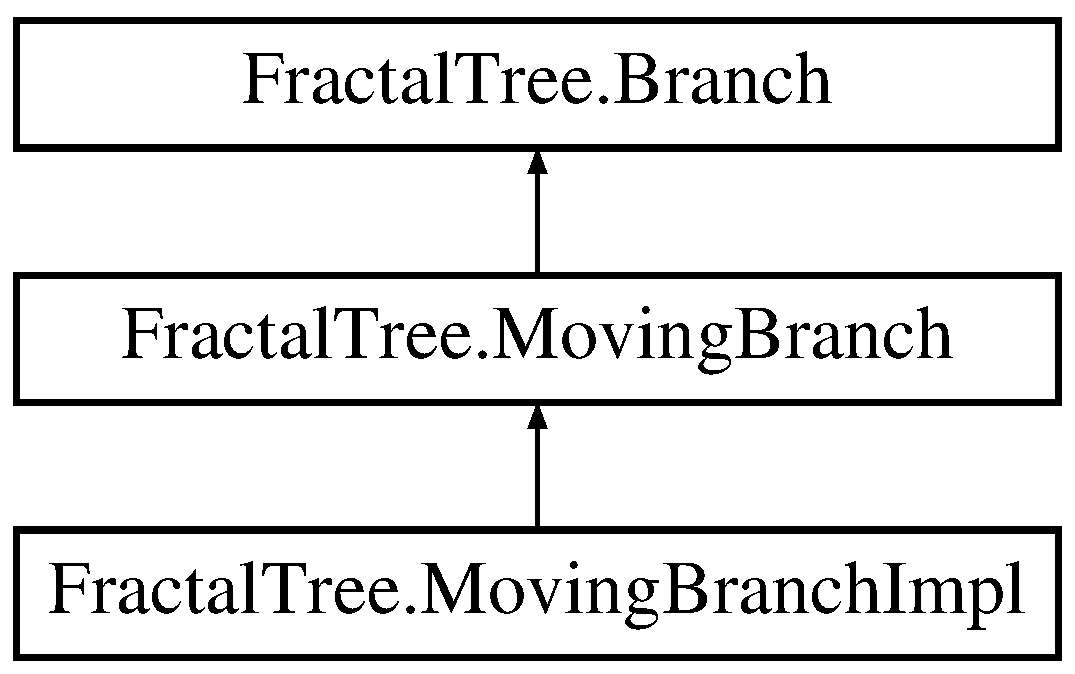
\includegraphics[height=3.000000cm]{interface_fractal_tree_1_1_moving_branch}
\end{center}
\end{figure}
\subsection*{Properties}
\begin{DoxyCompactItemize}
\item 
\hyperlink{class_fractal_tree_1_1_point_mass}{Point\+Mass} \hyperlink{interface_fractal_tree_1_1_moving_branch_afbf74eadb94a987e4f845e77b8d0b964}{start\+Point}\hspace{0.3cm}{\ttfamily  \mbox{[}get\mbox{]}}
\begin{DoxyCompactList}\small\item\em Gets the start point mass. Used to add spring force \end{DoxyCompactList}\item 
\hyperlink{class_fractal_tree_1_1_point_mass}{Point\+Mass} \hyperlink{interface_fractal_tree_1_1_moving_branch_a232ab0d1d87bb5a0abc5c54d4f26fe2b}{end\+Point}\hspace{0.3cm}{\ttfamily  \mbox{[}get\mbox{]}}
\begin{DoxyCompactList}\small\item\em Gets the end point mass. Used to add spring force. \end{DoxyCompactList}\end{DoxyCompactItemize}
\subsection*{Additional Inherited Members}


\subsection{Detailed Description}
Extends branch with point data for moving branches. 



\subsection{Property Documentation}
\mbox{\Hypertarget{interface_fractal_tree_1_1_moving_branch_a232ab0d1d87bb5a0abc5c54d4f26fe2b}\label{interface_fractal_tree_1_1_moving_branch_a232ab0d1d87bb5a0abc5c54d4f26fe2b}} 
\index{Fractal\+Tree\+::\+Moving\+Branch@{Fractal\+Tree\+::\+Moving\+Branch}!end\+Point@{end\+Point}}
\index{end\+Point@{end\+Point}!Fractal\+Tree\+::\+Moving\+Branch@{Fractal\+Tree\+::\+Moving\+Branch}}
\subsubsection{\texorpdfstring{end\+Point}{endPoint}}
{\footnotesize\ttfamily \hyperlink{class_fractal_tree_1_1_point_mass}{Point\+Mass} Fractal\+Tree.\+Moving\+Branch.\+end\+Point\hspace{0.3cm}{\ttfamily [get]}}



Gets the end point mass. Used to add spring force. 

The end point.\mbox{\Hypertarget{interface_fractal_tree_1_1_moving_branch_afbf74eadb94a987e4f845e77b8d0b964}\label{interface_fractal_tree_1_1_moving_branch_afbf74eadb94a987e4f845e77b8d0b964}} 
\index{Fractal\+Tree\+::\+Moving\+Branch@{Fractal\+Tree\+::\+Moving\+Branch}!start\+Point@{start\+Point}}
\index{start\+Point@{start\+Point}!Fractal\+Tree\+::\+Moving\+Branch@{Fractal\+Tree\+::\+Moving\+Branch}}
\subsubsection{\texorpdfstring{start\+Point}{startPoint}}
{\footnotesize\ttfamily \hyperlink{class_fractal_tree_1_1_point_mass}{Point\+Mass} Fractal\+Tree.\+Moving\+Branch.\+start\+Point\hspace{0.3cm}{\ttfamily [get]}}



Gets the start point mass. Used to add spring force 

The start point.

The documentation for this interface was generated from the following file\+:\begin{DoxyCompactItemize}
\item 
F\+T/\+Scripts/\+Branch/Branch.\+cs\end{DoxyCompactItemize}

\hypertarget{class_fractal_tree_1_1_moving_branch_impl}{}\section{Fractal\+Tree.\+Moving\+Branch\+Impl Class Reference}
\label{class_fractal_tree_1_1_moving_branch_impl}\index{Fractal\+Tree.\+Moving\+Branch\+Impl@{Fractal\+Tree.\+Moving\+Branch\+Impl}}


Extends a normal branch and adds spring functionality. Force can be applied to the start and end point of the branch.  


Inheritance diagram for Fractal\+Tree.\+Moving\+Branch\+Impl\+:\begin{figure}[H]
\begin{center}
\leavevmode
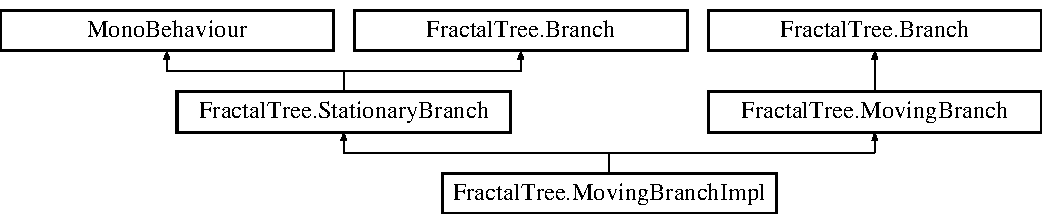
\includegraphics[height=2.871795cm]{class_fractal_tree_1_1_moving_branch_impl}
\end{center}
\end{figure}
\subsection*{Public Member Functions}
\begin{DoxyCompactItemize}
\item 
override void \hyperlink{class_fractal_tree_1_1_moving_branch_impl_a52861b34bb8a9550c6790bab90509660}{Setup} (\hyperlink{interface_fractal_tree_1_1_branch}{Branch} owner, Vector2 end, float thickness, Color \hyperlink{class_fractal_tree_1_1_stationary_branch_a265ca67d50299986adb192386fc7b932}{color})
\begin{DoxyCompactList}\small\item\em Setup the specified owner, end, thickness and color. Used to create a branch that is attached to another branch. \end{DoxyCompactList}\item 
override void \hyperlink{class_fractal_tree_1_1_moving_branch_impl_a73649451c7fbfa0793e0a1528e301215}{Setup} (\hyperlink{interface_fractal_tree_1_1_branch}{Branch} owner, Vector2 end, float thickness, Color \hyperlink{class_fractal_tree_1_1_stationary_branch_a265ca67d50299986adb192386fc7b932}{color}, bool auto\+Mass)
\begin{DoxyCompactList}\small\item\em Setup the specified owner, end, thickness and color. Used to create a branch that is attached to another branch that has its mass autogenerated based on line width. \end{DoxyCompactList}\item 
override void \hyperlink{class_fractal_tree_1_1_moving_branch_impl_aeea52b05117e613e0dd6c9ee5fbafb58}{Setup} (Vector2 start, Vector2 end, float thickness, Color \hyperlink{class_fractal_tree_1_1_stationary_branch_a265ca67d50299986adb192386fc7b932}{color})
\begin{DoxyCompactList}\small\item\em Setup the specified owner, end, thickness and color. Used to create a branch that is attached to another branch. \end{DoxyCompactList}\item 
override void \hyperlink{class_fractal_tree_1_1_moving_branch_impl_a4e7cde65899abaf121a906d06874c330}{Setup} (Vector2 start, Vector2 end, float width, Color \hyperlink{class_fractal_tree_1_1_stationary_branch_a265ca67d50299986adb192386fc7b932}{color}, bool auto\+Mass)
\begin{DoxyCompactList}\small\item\em Setup the specified owner, end, thickness and color. Used to create a branch that is attached to another branch that has its mass autogenerated based on line width. \end{DoxyCompactList}\item 
new T \hyperlink{class_fractal_tree_1_1_moving_branch_impl_a7f7776446fa70aac8efb669f9e41a4af}{Do\+Branching$<$ T $>$} (float angle)
\begin{DoxyCompactList}\small\item\em Returns a new branch based on current branch angle plus parameter angle. \end{DoxyCompactList}\end{DoxyCompactItemize}
\subsection*{Protected Member Functions}
\begin{DoxyCompactItemize}
\item 
\mbox{\Hypertarget{class_fractal_tree_1_1_moving_branch_impl_adf817bef89fca3d8a86c9c6197cb0f95}\label{class_fractal_tree_1_1_moving_branch_impl_adf817bef89fca3d8a86c9c6197cb0f95}} 
override void {\bfseries Awake} ()
\end{DoxyCompactItemize}
\subsection*{Properties}
\begin{DoxyCompactItemize}
\item 
\hyperlink{class_fractal_tree_1_1_point_mass}{Point\+Mass} \hyperlink{class_fractal_tree_1_1_moving_branch_impl_a360370cd5f0fb613596cb8d0fe942ffe}{start\+Point}\hspace{0.3cm}{\ttfamily  \mbox{[}get\mbox{]}}
\begin{DoxyCompactList}\small\item\em Gets the start point mass. Used to add spring force \end{DoxyCompactList}\item 
\hyperlink{class_fractal_tree_1_1_point_mass}{Point\+Mass} \hyperlink{class_fractal_tree_1_1_moving_branch_impl_aa2f492300936b8d8ce786050a5b7f2df}{end\+Point}\hspace{0.3cm}{\ttfamily  \mbox{[}get\mbox{]}}
\begin{DoxyCompactList}\small\item\em Gets the end point mass. Used to add spring force. \end{DoxyCompactList}\item 
override Vector2 \hyperlink{class_fractal_tree_1_1_moving_branch_impl_a520d7fca22147e6a552b4c4f2b946259}{start\+Pos}\hspace{0.3cm}{\ttfamily  \mbox{[}get\mbox{]}}
\begin{DoxyCompactList}\small\item\em Gets the start position. \end{DoxyCompactList}\item 
override Vector2 \hyperlink{class_fractal_tree_1_1_moving_branch_impl_a76ba4f9f3d3cad097bfa39f423775423}{end\+Pos}\hspace{0.3cm}{\ttfamily  \mbox{[}get\mbox{]}}
\begin{DoxyCompactList}\small\item\em Gets the end position. \end{DoxyCompactList}\end{DoxyCompactItemize}
\subsection*{Additional Inherited Members}


\subsection{Detailed Description}
Extends a normal branch and adds spring functionality. Force can be applied to the start and end point of the branch. 



\subsection{Member Function Documentation}
\mbox{\Hypertarget{class_fractal_tree_1_1_moving_branch_impl_a7f7776446fa70aac8efb669f9e41a4af}\label{class_fractal_tree_1_1_moving_branch_impl_a7f7776446fa70aac8efb669f9e41a4af}} 
\index{Fractal\+Tree\+::\+Moving\+Branch\+Impl@{Fractal\+Tree\+::\+Moving\+Branch\+Impl}!Do\+Branching$<$ T $>$@{Do\+Branching$<$ T $>$}}
\index{Do\+Branching$<$ T $>$@{Do\+Branching$<$ T $>$}!Fractal\+Tree\+::\+Moving\+Branch\+Impl@{Fractal\+Tree\+::\+Moving\+Branch\+Impl}}
\subsubsection{\texorpdfstring{Do\+Branching$<$ T $>$()}{DoBranching< T >()}}
{\footnotesize\ttfamily new T Fractal\+Tree.\+Moving\+Branch\+Impl.\+Do\+Branching$<$ T $>$ (\begin{DoxyParamCaption}\item[{float}]{angle }\end{DoxyParamCaption})}



Returns a new branch based on current branch angle plus parameter angle. 

\begin{DoxyReturn}{Returns}
The branching.
\end{DoxyReturn}

\begin{DoxyParams}{Parameters}
{\em angle} & Angle.\\
\hline
\end{DoxyParams}

\begin{DoxyTemplParams}{Template Parameters}
{\em T} & The 1st type parameter.\\
\hline
\end{DoxyTemplParams}


Implements \hyperlink{interface_fractal_tree_1_1_branch_ad3240d5e5d13df2ee22e55892f9c03cd}{Fractal\+Tree.\+Branch}.

\begin{Desc}
\item[Type Constraints]\begin{description}
\item[{\em T} : {\em Branch}]\end{description}
\end{Desc}
\mbox{\Hypertarget{class_fractal_tree_1_1_moving_branch_impl_a52861b34bb8a9550c6790bab90509660}\label{class_fractal_tree_1_1_moving_branch_impl_a52861b34bb8a9550c6790bab90509660}} 
\index{Fractal\+Tree\+::\+Moving\+Branch\+Impl@{Fractal\+Tree\+::\+Moving\+Branch\+Impl}!Setup@{Setup}}
\index{Setup@{Setup}!Fractal\+Tree\+::\+Moving\+Branch\+Impl@{Fractal\+Tree\+::\+Moving\+Branch\+Impl}}
\subsubsection{\texorpdfstring{Setup()}{Setup()}\hspace{0.1cm}{\footnotesize\ttfamily [1/4]}}
{\footnotesize\ttfamily override void Fractal\+Tree.\+Moving\+Branch\+Impl.\+Setup (\begin{DoxyParamCaption}\item[{\hyperlink{interface_fractal_tree_1_1_branch}{Branch}}]{owner,  }\item[{Vector2}]{end,  }\item[{float}]{thickness,  }\item[{Color}]{color }\end{DoxyParamCaption})\hspace{0.3cm}{\ttfamily [virtual]}}



Setup the specified owner, end, thickness and color. Used to create a branch that is attached to another branch. 


\begin{DoxyParams}{Parameters}
{\em owner} & The attached branch.\\
\hline
{\em end} & End.\\
\hline
{\em thickness} & Thickness.\\
\hline
{\em color} & Color.\\
\hline
\end{DoxyParams}


Reimplemented from \hyperlink{class_fractal_tree_1_1_stationary_branch_acaa0bef74389db9f1a2f57af38557000}{Fractal\+Tree.\+Stationary\+Branch}.

\mbox{\Hypertarget{class_fractal_tree_1_1_moving_branch_impl_a73649451c7fbfa0793e0a1528e301215}\label{class_fractal_tree_1_1_moving_branch_impl_a73649451c7fbfa0793e0a1528e301215}} 
\index{Fractal\+Tree\+::\+Moving\+Branch\+Impl@{Fractal\+Tree\+::\+Moving\+Branch\+Impl}!Setup@{Setup}}
\index{Setup@{Setup}!Fractal\+Tree\+::\+Moving\+Branch\+Impl@{Fractal\+Tree\+::\+Moving\+Branch\+Impl}}
\subsubsection{\texorpdfstring{Setup()}{Setup()}\hspace{0.1cm}{\footnotesize\ttfamily [2/4]}}
{\footnotesize\ttfamily override void Fractal\+Tree.\+Moving\+Branch\+Impl.\+Setup (\begin{DoxyParamCaption}\item[{\hyperlink{interface_fractal_tree_1_1_branch}{Branch}}]{owner,  }\item[{Vector2}]{end,  }\item[{float}]{thickness,  }\item[{Color}]{color,  }\item[{bool}]{auto\+Mass }\end{DoxyParamCaption})\hspace{0.3cm}{\ttfamily [virtual]}}



Setup the specified owner, end, thickness and color. Used to create a branch that is attached to another branch that has its mass autogenerated based on line width. 


\begin{DoxyParams}{Parameters}
{\em owner} & Owner.\\
\hline
{\em end} & End.\\
\hline
{\em thickness} & Thickness.\\
\hline
{\em color} & Color.\\
\hline
{\em auto\+Mass} & If set to {\ttfamily true} auto mass.\\
\hline
\end{DoxyParams}


Reimplemented from \hyperlink{class_fractal_tree_1_1_stationary_branch_a262c5810fadbd2c8aea1f2afdca57126}{Fractal\+Tree.\+Stationary\+Branch}.

\mbox{\Hypertarget{class_fractal_tree_1_1_moving_branch_impl_aeea52b05117e613e0dd6c9ee5fbafb58}\label{class_fractal_tree_1_1_moving_branch_impl_aeea52b05117e613e0dd6c9ee5fbafb58}} 
\index{Fractal\+Tree\+::\+Moving\+Branch\+Impl@{Fractal\+Tree\+::\+Moving\+Branch\+Impl}!Setup@{Setup}}
\index{Setup@{Setup}!Fractal\+Tree\+::\+Moving\+Branch\+Impl@{Fractal\+Tree\+::\+Moving\+Branch\+Impl}}
\subsubsection{\texorpdfstring{Setup()}{Setup()}\hspace{0.1cm}{\footnotesize\ttfamily [3/4]}}
{\footnotesize\ttfamily override void Fractal\+Tree.\+Moving\+Branch\+Impl.\+Setup (\begin{DoxyParamCaption}\item[{Vector2}]{start,  }\item[{Vector2}]{end,  }\item[{float}]{thickness,  }\item[{Color}]{color }\end{DoxyParamCaption})\hspace{0.3cm}{\ttfamily [virtual]}}



Setup the specified owner, end, thickness and color. Used to create a branch that is attached to another branch. 


\begin{DoxyParams}{Parameters}
{\em owner} & The attached branch.\\
\hline
{\em end} & End.\\
\hline
{\em thickness} & Thickness.\\
\hline
{\em color} & Color.\\
\hline
{\em start} & Start.\\
\hline
\end{DoxyParams}


Reimplemented from \hyperlink{class_fractal_tree_1_1_stationary_branch_a62e1aa7062ef70a8726dfe21a9e28d76}{Fractal\+Tree.\+Stationary\+Branch}.

\mbox{\Hypertarget{class_fractal_tree_1_1_moving_branch_impl_a4e7cde65899abaf121a906d06874c330}\label{class_fractal_tree_1_1_moving_branch_impl_a4e7cde65899abaf121a906d06874c330}} 
\index{Fractal\+Tree\+::\+Moving\+Branch\+Impl@{Fractal\+Tree\+::\+Moving\+Branch\+Impl}!Setup@{Setup}}
\index{Setup@{Setup}!Fractal\+Tree\+::\+Moving\+Branch\+Impl@{Fractal\+Tree\+::\+Moving\+Branch\+Impl}}
\subsubsection{\texorpdfstring{Setup()}{Setup()}\hspace{0.1cm}{\footnotesize\ttfamily [4/4]}}
{\footnotesize\ttfamily override void Fractal\+Tree.\+Moving\+Branch\+Impl.\+Setup (\begin{DoxyParamCaption}\item[{Vector2}]{start,  }\item[{Vector2}]{end,  }\item[{float}]{width,  }\item[{Color}]{color,  }\item[{bool}]{auto\+Mass }\end{DoxyParamCaption})\hspace{0.3cm}{\ttfamily [virtual]}}



Setup the specified owner, end, thickness and color. Used to create a branch that is attached to another branch that has its mass autogenerated based on line width. 


\begin{DoxyParams}{Parameters}
{\em owner} & Owner.\\
\hline
{\em end} & End.\\
\hline
{\em thickness} & Thickness.\\
\hline
{\em color} & Color.\\
\hline
{\em start} & Start.\\
\hline
{\em width} & Width.\\
\hline
{\em auto\+Mass} & If set to {\ttfamily true} auto mass.\\
\hline
\end{DoxyParams}


Reimplemented from \hyperlink{class_fractal_tree_1_1_stationary_branch_a61cfd43bb83cf63bf1ad25f339866d7a}{Fractal\+Tree.\+Stationary\+Branch}.



\subsection{Property Documentation}
\mbox{\Hypertarget{class_fractal_tree_1_1_moving_branch_impl_aa2f492300936b8d8ce786050a5b7f2df}\label{class_fractal_tree_1_1_moving_branch_impl_aa2f492300936b8d8ce786050a5b7f2df}} 
\index{Fractal\+Tree\+::\+Moving\+Branch\+Impl@{Fractal\+Tree\+::\+Moving\+Branch\+Impl}!end\+Point@{end\+Point}}
\index{end\+Point@{end\+Point}!Fractal\+Tree\+::\+Moving\+Branch\+Impl@{Fractal\+Tree\+::\+Moving\+Branch\+Impl}}
\subsubsection{\texorpdfstring{end\+Point}{endPoint}}
{\footnotesize\ttfamily \hyperlink{class_fractal_tree_1_1_point_mass}{Point\+Mass} Fractal\+Tree.\+Moving\+Branch\+Impl.\+end\+Point\hspace{0.3cm}{\ttfamily [get]}}



Gets the end point mass. Used to add spring force. 

The end point.\mbox{\Hypertarget{class_fractal_tree_1_1_moving_branch_impl_a76ba4f9f3d3cad097bfa39f423775423}\label{class_fractal_tree_1_1_moving_branch_impl_a76ba4f9f3d3cad097bfa39f423775423}} 
\index{Fractal\+Tree\+::\+Moving\+Branch\+Impl@{Fractal\+Tree\+::\+Moving\+Branch\+Impl}!end\+Pos@{end\+Pos}}
\index{end\+Pos@{end\+Pos}!Fractal\+Tree\+::\+Moving\+Branch\+Impl@{Fractal\+Tree\+::\+Moving\+Branch\+Impl}}
\subsubsection{\texorpdfstring{end\+Pos}{endPos}}
{\footnotesize\ttfamily override Vector2 Fractal\+Tree.\+Moving\+Branch\+Impl.\+end\+Pos\hspace{0.3cm}{\ttfamily [get]}}



Gets the end position. 

The end position.\mbox{\Hypertarget{class_fractal_tree_1_1_moving_branch_impl_a360370cd5f0fb613596cb8d0fe942ffe}\label{class_fractal_tree_1_1_moving_branch_impl_a360370cd5f0fb613596cb8d0fe942ffe}} 
\index{Fractal\+Tree\+::\+Moving\+Branch\+Impl@{Fractal\+Tree\+::\+Moving\+Branch\+Impl}!start\+Point@{start\+Point}}
\index{start\+Point@{start\+Point}!Fractal\+Tree\+::\+Moving\+Branch\+Impl@{Fractal\+Tree\+::\+Moving\+Branch\+Impl}}
\subsubsection{\texorpdfstring{start\+Point}{startPoint}}
{\footnotesize\ttfamily \hyperlink{class_fractal_tree_1_1_point_mass}{Point\+Mass} Fractal\+Tree.\+Moving\+Branch\+Impl.\+start\+Point\hspace{0.3cm}{\ttfamily [get]}}



Gets the start point mass. Used to add spring force 

The start point.\mbox{\Hypertarget{class_fractal_tree_1_1_moving_branch_impl_a520d7fca22147e6a552b4c4f2b946259}\label{class_fractal_tree_1_1_moving_branch_impl_a520d7fca22147e6a552b4c4f2b946259}} 
\index{Fractal\+Tree\+::\+Moving\+Branch\+Impl@{Fractal\+Tree\+::\+Moving\+Branch\+Impl}!start\+Pos@{start\+Pos}}
\index{start\+Pos@{start\+Pos}!Fractal\+Tree\+::\+Moving\+Branch\+Impl@{Fractal\+Tree\+::\+Moving\+Branch\+Impl}}
\subsubsection{\texorpdfstring{start\+Pos}{startPos}}
{\footnotesize\ttfamily override Vector2 Fractal\+Tree.\+Moving\+Branch\+Impl.\+start\+Pos\hspace{0.3cm}{\ttfamily [get]}}



Gets the start position. 

The start position.

The documentation for this class was generated from the following file\+:\begin{DoxyCompactItemize}
\item 
F\+T/\+Scripts/\+Branch/Moving\+Branch\+Impl.\+cs\end{DoxyCompactItemize}

\hypertarget{class_fractal_tree_1_1_moving_tree_builder}{}\section{Fractal\+Tree.\+Moving\+Tree\+Builder Class Reference}
\label{class_fractal_tree_1_1_moving_tree_builder}\index{Fractal\+Tree.\+Moving\+Tree\+Builder@{Fractal\+Tree.\+Moving\+Tree\+Builder}}
Inheritance diagram for Fractal\+Tree.\+Moving\+Tree\+Builder\+:\begin{figure}[H]
\begin{center}
\leavevmode
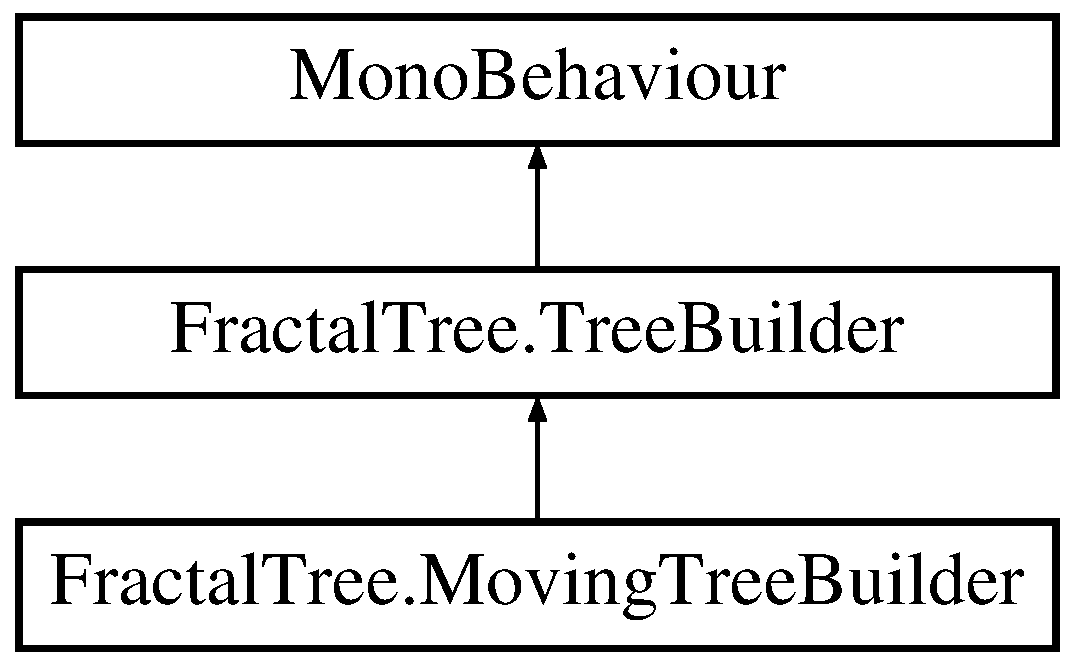
\includegraphics[height=3.000000cm]{class_fractal_tree_1_1_moving_tree_builder}
\end{center}
\end{figure}
\subsection*{Public Member Functions}
\begin{DoxyCompactItemize}
\item 
override void \hyperlink{class_fractal_tree_1_1_moving_tree_builder_a4c58924b1d19c896cd1af1256ce242eb}{Build} ()
\begin{DoxyCompactList}\small\item\em Build this instance. \end{DoxyCompactList}\item 
void \hyperlink{class_fractal_tree_1_1_moving_tree_builder_a7da9440aa0482b959854bb28ff281a9a}{Apply\+Directed\+Force} (Vector2 force, Vector2 position, float radius)
\begin{DoxyCompactList}\small\item\em Applies a directed force to all branches within range. \end{DoxyCompactList}\item 
void \hyperlink{class_fractal_tree_1_1_moving_tree_builder_aac060965e91832c1dfefd94b7c9b152b}{Apply\+Push\+Force} (float force, Vector2 position, float radius)
\begin{DoxyCompactList}\small\item\em Applies a push force to all branches within range. \end{DoxyCompactList}\item 
void \hyperlink{class_fractal_tree_1_1_moving_tree_builder_ace24108b660cb1dcebb609eef51588ed}{Apply\+Pull\+Force} (float force, Vector2 position, float radius)
\begin{DoxyCompactList}\small\item\em Applies a pull force to all branches in range. \end{DoxyCompactList}\end{DoxyCompactItemize}
\subsection*{Properties}
\begin{DoxyCompactItemize}
\item 
List$<$ \hyperlink{interface_fractal_tree_1_1_moving_branch}{Moving\+Branch} $>$ \hyperlink{class_fractal_tree_1_1_moving_tree_builder_aca75f30f0c8170efd0b62eca6eee9e00}{branches}\hspace{0.3cm}{\ttfamily  \mbox{[}get\mbox{]}}
\begin{DoxyCompactList}\small\item\em A list of all branches associated with the tree. \end{DoxyCompactList}\end{DoxyCompactItemize}
\subsection*{Additional Inherited Members}


\subsection{Member Function Documentation}
\hypertarget{class_fractal_tree_1_1_moving_tree_builder_a7da9440aa0482b959854bb28ff281a9a}{}\label{class_fractal_tree_1_1_moving_tree_builder_a7da9440aa0482b959854bb28ff281a9a} 
\index{Fractal\+Tree\+::\+Moving\+Tree\+Builder@{Fractal\+Tree\+::\+Moving\+Tree\+Builder}!Apply\+Directed\+Force@{Apply\+Directed\+Force}}
\index{Apply\+Directed\+Force@{Apply\+Directed\+Force}!Fractal\+Tree\+::\+Moving\+Tree\+Builder@{Fractal\+Tree\+::\+Moving\+Tree\+Builder}}
\subsubsection{\texorpdfstring{Apply\+Directed\+Force()}{ApplyDirectedForce()}}
{\footnotesize\ttfamily void Fractal\+Tree.\+Moving\+Tree\+Builder.\+Apply\+Directed\+Force (\begin{DoxyParamCaption}\item[{Vector2}]{force,  }\item[{Vector2}]{position,  }\item[{float}]{radius }\end{DoxyParamCaption})}



Applies a directed force to all branches within range. 


\begin{DoxyParams}{Parameters}
{\em force} & Force.\\
\hline
{\em position} & Position.\\
\hline
{\em radius} & Radius.\\
\hline
\end{DoxyParams}
\hypertarget{class_fractal_tree_1_1_moving_tree_builder_ace24108b660cb1dcebb609eef51588ed}{}\label{class_fractal_tree_1_1_moving_tree_builder_ace24108b660cb1dcebb609eef51588ed} 
\index{Fractal\+Tree\+::\+Moving\+Tree\+Builder@{Fractal\+Tree\+::\+Moving\+Tree\+Builder}!Apply\+Pull\+Force@{Apply\+Pull\+Force}}
\index{Apply\+Pull\+Force@{Apply\+Pull\+Force}!Fractal\+Tree\+::\+Moving\+Tree\+Builder@{Fractal\+Tree\+::\+Moving\+Tree\+Builder}}
\subsubsection{\texorpdfstring{Apply\+Pull\+Force()}{ApplyPullForce()}}
{\footnotesize\ttfamily void Fractal\+Tree.\+Moving\+Tree\+Builder.\+Apply\+Pull\+Force (\begin{DoxyParamCaption}\item[{float}]{force,  }\item[{Vector2}]{position,  }\item[{float}]{radius }\end{DoxyParamCaption})}



Applies a pull force to all branches in range. 


\begin{DoxyParams}{Parameters}
{\em force} & Force.\\
\hline
{\em position} & Position.\\
\hline
{\em radius} & Radius.\\
\hline
\end{DoxyParams}
\hypertarget{class_fractal_tree_1_1_moving_tree_builder_aac060965e91832c1dfefd94b7c9b152b}{}\label{class_fractal_tree_1_1_moving_tree_builder_aac060965e91832c1dfefd94b7c9b152b} 
\index{Fractal\+Tree\+::\+Moving\+Tree\+Builder@{Fractal\+Tree\+::\+Moving\+Tree\+Builder}!Apply\+Push\+Force@{Apply\+Push\+Force}}
\index{Apply\+Push\+Force@{Apply\+Push\+Force}!Fractal\+Tree\+::\+Moving\+Tree\+Builder@{Fractal\+Tree\+::\+Moving\+Tree\+Builder}}
\subsubsection{\texorpdfstring{Apply\+Push\+Force()}{ApplyPushForce()}}
{\footnotesize\ttfamily void Fractal\+Tree.\+Moving\+Tree\+Builder.\+Apply\+Push\+Force (\begin{DoxyParamCaption}\item[{float}]{force,  }\item[{Vector2}]{position,  }\item[{float}]{radius }\end{DoxyParamCaption})}



Applies a push force to all branches within range. 


\begin{DoxyParams}{Parameters}
{\em force} & Force.\\
\hline
{\em position} & Position.\\
\hline
{\em radius} & Radius.\\
\hline
\end{DoxyParams}
\hypertarget{class_fractal_tree_1_1_moving_tree_builder_a4c58924b1d19c896cd1af1256ce242eb}{}\label{class_fractal_tree_1_1_moving_tree_builder_a4c58924b1d19c896cd1af1256ce242eb} 
\index{Fractal\+Tree\+::\+Moving\+Tree\+Builder@{Fractal\+Tree\+::\+Moving\+Tree\+Builder}!Build@{Build}}
\index{Build@{Build}!Fractal\+Tree\+::\+Moving\+Tree\+Builder@{Fractal\+Tree\+::\+Moving\+Tree\+Builder}}
\subsubsection{\texorpdfstring{Build()}{Build()}}
{\footnotesize\ttfamily override void Fractal\+Tree.\+Moving\+Tree\+Builder.\+Build (\begin{DoxyParamCaption}{ }\end{DoxyParamCaption})\hspace{0.3cm}{\ttfamily [virtual]}}



Build this instance. 



Implements \hyperlink{class_fractal_tree_1_1_tree_builder}{Fractal\+Tree.\+Tree\+Builder}.



\subsection{Property Documentation}
\hypertarget{class_fractal_tree_1_1_moving_tree_builder_aca75f30f0c8170efd0b62eca6eee9e00}{}\label{class_fractal_tree_1_1_moving_tree_builder_aca75f30f0c8170efd0b62eca6eee9e00} 
\index{Fractal\+Tree\+::\+Moving\+Tree\+Builder@{Fractal\+Tree\+::\+Moving\+Tree\+Builder}!branches@{branches}}
\index{branches@{branches}!Fractal\+Tree\+::\+Moving\+Tree\+Builder@{Fractal\+Tree\+::\+Moving\+Tree\+Builder}}
\subsubsection{\texorpdfstring{branches}{branches}}
{\footnotesize\ttfamily List$<$\hyperlink{interface_fractal_tree_1_1_moving_branch}{Moving\+Branch}$>$ Fractal\+Tree.\+Moving\+Tree\+Builder.\+branches\hspace{0.3cm}{\ttfamily [get]}}



A list of all branches associated with the tree. 

The branches.

The documentation for this class was generated from the following file\+:\begin{DoxyCompactItemize}
\item 
Moving\+Tree\+Builder.\+cs\end{DoxyCompactItemize}

\hypertarget{class_fractal_tree_1_1_moving_tree_builder_editor}{}\section{Fractal\+Tree.\+Moving\+Tree\+Builder\+Editor Class Reference}
\label{class_fractal_tree_1_1_moving_tree_builder_editor}\index{Fractal\+Tree.\+Moving\+Tree\+Builder\+Editor@{Fractal\+Tree.\+Moving\+Tree\+Builder\+Editor}}
Inheritance diagram for Fractal\+Tree.\+Moving\+Tree\+Builder\+Editor\+:\begin{figure}[H]
\begin{center}
\leavevmode
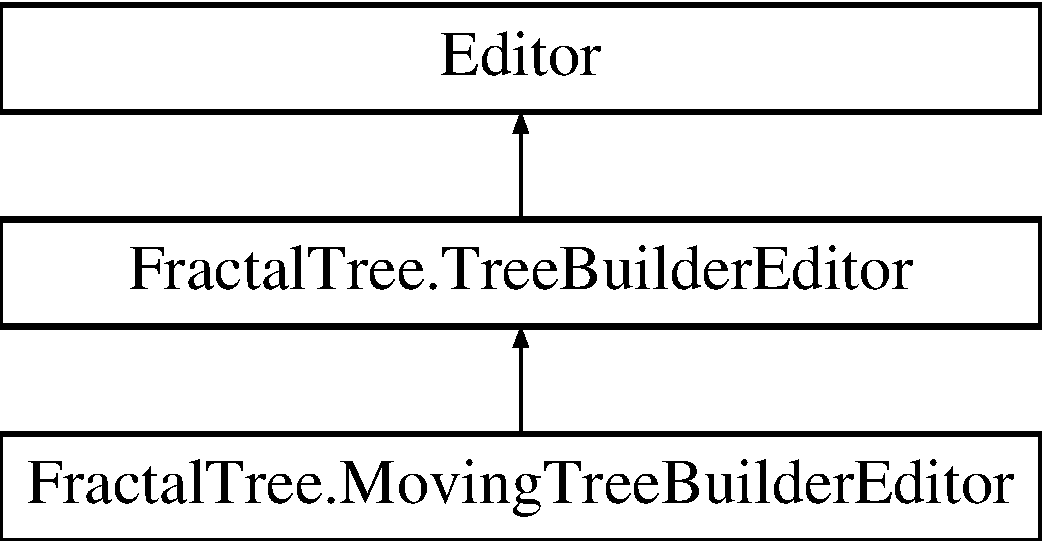
\includegraphics[height=3.000000cm]{class_fractal_tree_1_1_moving_tree_builder_editor}
\end{center}
\end{figure}
\subsection*{Public Member Functions}
\begin{DoxyCompactItemize}
\item 
\mbox{\Hypertarget{class_fractal_tree_1_1_moving_tree_builder_editor_ad14f3f2ae40f63659f883898b910f7aa}\label{class_fractal_tree_1_1_moving_tree_builder_editor_ad14f3f2ae40f63659f883898b910f7aa}} 
override void {\bfseries On\+Inspector\+G\+UI} ()
\end{DoxyCompactItemize}
\subsection*{Additional Inherited Members}


The documentation for this class was generated from the following file\+:\begin{DoxyCompactItemize}
\item 
F\+T/\+Scripts/\+Editor/Moving\+Tree\+Builder\+Editor.\+cs\end{DoxyCompactItemize}

\hypertarget{class_fractal_tree_1_1_point_mass}{}\section{Fractal\+Tree.\+Point\+Mass Class Reference}
\label{class_fractal_tree_1_1_point_mass}\index{Fractal\+Tree.\+Point\+Mass@{Fractal\+Tree.\+Point\+Mass}}


Added to the start and end of movable branches. Used to add spring force to a branch.  


\subsection*{Public Member Functions}
\begin{DoxyCompactItemize}
\item 
\hyperlink{class_fractal_tree_1_1_point_mass_aeae7254d48ee357290cc926783f76232}{Point\+Mass} (Vector2 \hyperlink{class_fractal_tree_1_1_point_mass_a388c55b55d073a8962d8c4e61ce4fd94}{position}, float inv\+Mass, float bounce\+Back\+Force)
\begin{DoxyCompactList}\small\item\em Initializes a new instance of the \hyperlink{class_fractal_tree_1_1_point_mass}{Fractal\+Tree.\+Point\+Mass} class. \end{DoxyCompactList}\item 
void \hyperlink{class_fractal_tree_1_1_point_mass_a6f5491d604a47a8dd4c2c26d349e618f}{Apply\+Force} (Vector2 force)
\begin{DoxyCompactList}\small\item\em Applies a force. \end{DoxyCompactList}\item 
void \hyperlink{class_fractal_tree_1_1_point_mass_aaade3e27a4d89806c8c1357b3c498898}{Increase\+Damping} (float factor)
\begin{DoxyCompactList}\small\item\em Increases the damping factor. This dampens the velocity each step. \end{DoxyCompactList}\item 
void \hyperlink{class_fractal_tree_1_1_point_mass_a376cf6a1c55c15a5ff8c504af6cd1ed7}{Do\+Update} ()
\begin{DoxyCompactList}\small\item\em Updates position based on current force and distance from initial position. \end{DoxyCompactList}\end{DoxyCompactItemize}
\subsection*{Properties}
\begin{DoxyCompactItemize}
\item 
Vector2 \hyperlink{class_fractal_tree_1_1_point_mass_a388c55b55d073a8962d8c4e61ce4fd94}{position}\hspace{0.3cm}{\ttfamily  \mbox{[}get, set\mbox{]}}
\begin{DoxyCompactList}\small\item\em T\+He current position of the branch point. \end{DoxyCompactList}\item 
Vector2 \hyperlink{class_fractal_tree_1_1_point_mass_a1cbd0cc0eacfadb549cbc5fdb87ccbb1}{velocity}\hspace{0.3cm}{\ttfamily  \mbox{[}get\mbox{]}}
\begin{DoxyCompactList}\small\item\em Gets the velocity. \end{DoxyCompactList}\item 
bool \hyperlink{class_fractal_tree_1_1_point_mass_a25ea2ddc370c2cf21b7f376bd8bb2cf6}{force\+Applied}\hspace{0.3cm}{\ttfamily  \mbox{[}get\mbox{]}}
\begin{DoxyCompactList}\small\item\em Gets a value indicating whether this \hyperlink{class_fractal_tree_1_1_point_mass}{Fractal\+Tree.\+Point\+Mass} has had a force applied. \end{DoxyCompactList}\end{DoxyCompactItemize}


\subsection{Detailed Description}
Added to the start and end of movable branches. Used to add spring force to a branch. 



\subsection{Constructor \& Destructor Documentation}
\hypertarget{class_fractal_tree_1_1_point_mass_aeae7254d48ee357290cc926783f76232}{}\label{class_fractal_tree_1_1_point_mass_aeae7254d48ee357290cc926783f76232} 
\index{Fractal\+Tree\+::\+Point\+Mass@{Fractal\+Tree\+::\+Point\+Mass}!Point\+Mass@{Point\+Mass}}
\index{Point\+Mass@{Point\+Mass}!Fractal\+Tree\+::\+Point\+Mass@{Fractal\+Tree\+::\+Point\+Mass}}
\subsubsection{\texorpdfstring{Point\+Mass()}{PointMass()}}
{\footnotesize\ttfamily Fractal\+Tree.\+Point\+Mass.\+Point\+Mass (\begin{DoxyParamCaption}\item[{Vector2}]{position,  }\item[{float}]{inv\+Mass,  }\item[{float}]{bounce\+Back\+Force }\end{DoxyParamCaption})}



Initializes a new instance of the \hyperlink{class_fractal_tree_1_1_point_mass}{Fractal\+Tree.\+Point\+Mass} class. 


\begin{DoxyParams}{Parameters}
{\em position} & Initial position.\\
\hline
{\em inv\+Mass} & Inverse mass, lower numbers result in more force required to move the point.\\
\hline
{\em bounce\+Back\+Force} & Bounce back force. The force applied when moving the spring back to its initial position. \\
\hline
\end{DoxyParams}


\subsection{Member Function Documentation}
\hypertarget{class_fractal_tree_1_1_point_mass_a6f5491d604a47a8dd4c2c26d349e618f}{}\label{class_fractal_tree_1_1_point_mass_a6f5491d604a47a8dd4c2c26d349e618f} 
\index{Fractal\+Tree\+::\+Point\+Mass@{Fractal\+Tree\+::\+Point\+Mass}!Apply\+Force@{Apply\+Force}}
\index{Apply\+Force@{Apply\+Force}!Fractal\+Tree\+::\+Point\+Mass@{Fractal\+Tree\+::\+Point\+Mass}}
\subsubsection{\texorpdfstring{Apply\+Force()}{ApplyForce()}}
{\footnotesize\ttfamily void Fractal\+Tree.\+Point\+Mass.\+Apply\+Force (\begin{DoxyParamCaption}\item[{Vector2}]{force }\end{DoxyParamCaption})}



Applies a force. 


\begin{DoxyParams}{Parameters}
{\em force} & Force.\\
\hline
\end{DoxyParams}
\hypertarget{class_fractal_tree_1_1_point_mass_a376cf6a1c55c15a5ff8c504af6cd1ed7}{}\label{class_fractal_tree_1_1_point_mass_a376cf6a1c55c15a5ff8c504af6cd1ed7} 
\index{Fractal\+Tree\+::\+Point\+Mass@{Fractal\+Tree\+::\+Point\+Mass}!Do\+Update@{Do\+Update}}
\index{Do\+Update@{Do\+Update}!Fractal\+Tree\+::\+Point\+Mass@{Fractal\+Tree\+::\+Point\+Mass}}
\subsubsection{\texorpdfstring{Do\+Update()}{DoUpdate()}}
{\footnotesize\ttfamily void Fractal\+Tree.\+Point\+Mass.\+Do\+Update (\begin{DoxyParamCaption}{ }\end{DoxyParamCaption})}



Updates position based on current force and distance from initial position. 

\hypertarget{class_fractal_tree_1_1_point_mass_aaade3e27a4d89806c8c1357b3c498898}{}\label{class_fractal_tree_1_1_point_mass_aaade3e27a4d89806c8c1357b3c498898} 
\index{Fractal\+Tree\+::\+Point\+Mass@{Fractal\+Tree\+::\+Point\+Mass}!Increase\+Damping@{Increase\+Damping}}
\index{Increase\+Damping@{Increase\+Damping}!Fractal\+Tree\+::\+Point\+Mass@{Fractal\+Tree\+::\+Point\+Mass}}
\subsubsection{\texorpdfstring{Increase\+Damping()}{IncreaseDamping()}}
{\footnotesize\ttfamily void Fractal\+Tree.\+Point\+Mass.\+Increase\+Damping (\begin{DoxyParamCaption}\item[{float}]{factor }\end{DoxyParamCaption})}



Increases the damping factor. This dampens the velocity each step. 


\begin{DoxyParams}{Parameters}
{\em factor} & Factor.\\
\hline
\end{DoxyParams}


\subsection{Property Documentation}
\hypertarget{class_fractal_tree_1_1_point_mass_a25ea2ddc370c2cf21b7f376bd8bb2cf6}{}\label{class_fractal_tree_1_1_point_mass_a25ea2ddc370c2cf21b7f376bd8bb2cf6} 
\index{Fractal\+Tree\+::\+Point\+Mass@{Fractal\+Tree\+::\+Point\+Mass}!force\+Applied@{force\+Applied}}
\index{force\+Applied@{force\+Applied}!Fractal\+Tree\+::\+Point\+Mass@{Fractal\+Tree\+::\+Point\+Mass}}
\subsubsection{\texorpdfstring{force\+Applied}{forceApplied}}
{\footnotesize\ttfamily bool Fractal\+Tree.\+Point\+Mass.\+force\+Applied\hspace{0.3cm}{\ttfamily [get]}}



Gets a value indicating whether this \hyperlink{class_fractal_tree_1_1_point_mass}{Fractal\+Tree.\+Point\+Mass} has had a force applied. 

{\ttfamily true} if force applied; otherwise, {\ttfamily false}.\hypertarget{class_fractal_tree_1_1_point_mass_a388c55b55d073a8962d8c4e61ce4fd94}{}\label{class_fractal_tree_1_1_point_mass_a388c55b55d073a8962d8c4e61ce4fd94} 
\index{Fractal\+Tree\+::\+Point\+Mass@{Fractal\+Tree\+::\+Point\+Mass}!position@{position}}
\index{position@{position}!Fractal\+Tree\+::\+Point\+Mass@{Fractal\+Tree\+::\+Point\+Mass}}
\subsubsection{\texorpdfstring{position}{position}}
{\footnotesize\ttfamily Vector2 Fractal\+Tree.\+Point\+Mass.\+position\hspace{0.3cm}{\ttfamily [get]}, {\ttfamily [set]}}



T\+He current position of the branch point. 

The position.\hypertarget{class_fractal_tree_1_1_point_mass_a1cbd0cc0eacfadb549cbc5fdb87ccbb1}{}\label{class_fractal_tree_1_1_point_mass_a1cbd0cc0eacfadb549cbc5fdb87ccbb1} 
\index{Fractal\+Tree\+::\+Point\+Mass@{Fractal\+Tree\+::\+Point\+Mass}!velocity@{velocity}}
\index{velocity@{velocity}!Fractal\+Tree\+::\+Point\+Mass@{Fractal\+Tree\+::\+Point\+Mass}}
\subsubsection{\texorpdfstring{velocity}{velocity}}
{\footnotesize\ttfamily Vector2 Fractal\+Tree.\+Point\+Mass.\+velocity\hspace{0.3cm}{\ttfamily [get]}}



Gets the velocity. 

The velocity.

The documentation for this class was generated from the following file\+:\begin{DoxyCompactItemize}
\item 
Point\+Mass.\+cs\end{DoxyCompactItemize}

\hypertarget{class_fractal_tree_1_1_spring}{}\section{Fractal\+Tree.\+Spring Class Reference}
\label{class_fractal_tree_1_1_spring}\index{Fractal\+Tree.\+Spring@{Fractal\+Tree.\+Spring}}


Connects two point masses and apllies a pull force to ensure points stay within a target length.  


Inheritance diagram for Fractal\+Tree.\+Spring\+:\begin{figure}[H]
\begin{center}
\leavevmode
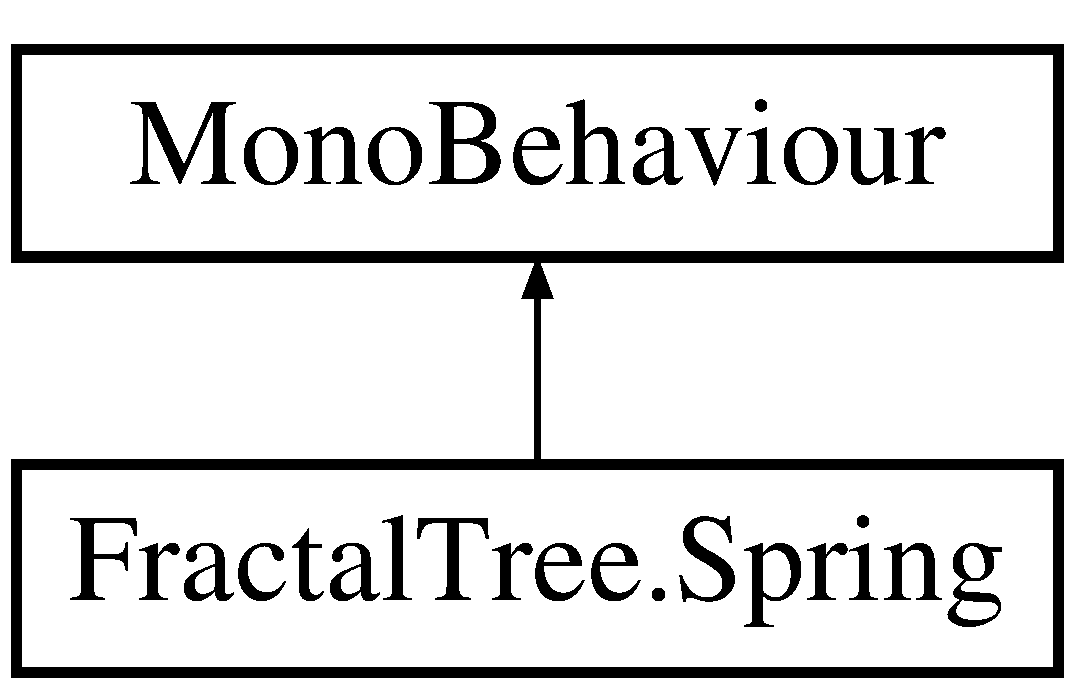
\includegraphics[height=2.000000cm]{class_fractal_tree_1_1_spring}
\end{center}
\end{figure}
\subsection*{Public Member Functions}
\begin{DoxyCompactItemize}
\item 
void \hyperlink{class_fractal_tree_1_1_spring_a49e3b32769c76e626650280f6016996d}{Setup} (\hyperlink{class_fractal_tree_1_1_point_mass}{Point\+Mass} \hyperlink{class_fractal_tree_1_1_spring_a4008f4f4f6404df50062047b0afa2ec8}{start}, \hyperlink{class_fractal_tree_1_1_point_mass}{Point\+Mass} \hyperlink{class_fractal_tree_1_1_spring_a22f6b5200ab129728b9fbb06b5faca1f}{end}, float stiffness, float damping)
\begin{DoxyCompactList}\small\item\em Setup the specified start, end, stiffness and damping. \end{DoxyCompactList}\item 
void \hyperlink{class_fractal_tree_1_1_spring_a38d6d4709c69509ef73c1725a53e470a}{Do\+Update} ()
\begin{DoxyCompactList}\small\item\em Applies force to start and point based on distance between points. \end{DoxyCompactList}\end{DoxyCompactItemize}
\subsection*{Public Attributes}
\begin{DoxyCompactItemize}
\item 
\hyperlink{class_fractal_tree_1_1_point_mass}{Point\+Mass} \hyperlink{class_fractal_tree_1_1_spring_a4008f4f4f6404df50062047b0afa2ec8}{start}
\begin{DoxyCompactList}\small\item\em The start point mass. \end{DoxyCompactList}\item 
\hyperlink{class_fractal_tree_1_1_point_mass}{Point\+Mass} \hyperlink{class_fractal_tree_1_1_spring_a22f6b5200ab129728b9fbb06b5faca1f}{end}
\begin{DoxyCompactList}\small\item\em The end point mass. \end{DoxyCompactList}\end{DoxyCompactItemize}


\subsection{Detailed Description}
Connects two point masses and apllies a pull force to ensure points stay within a target length. 



\subsection{Member Function Documentation}
\hypertarget{class_fractal_tree_1_1_spring_a38d6d4709c69509ef73c1725a53e470a}{}\label{class_fractal_tree_1_1_spring_a38d6d4709c69509ef73c1725a53e470a} 
\index{Fractal\+Tree\+::\+Spring@{Fractal\+Tree\+::\+Spring}!Do\+Update@{Do\+Update}}
\index{Do\+Update@{Do\+Update}!Fractal\+Tree\+::\+Spring@{Fractal\+Tree\+::\+Spring}}
\subsubsection{\texorpdfstring{Do\+Update()}{DoUpdate()}}
{\footnotesize\ttfamily void Fractal\+Tree.\+Spring.\+Do\+Update (\begin{DoxyParamCaption}{ }\end{DoxyParamCaption})}



Applies force to start and point based on distance between points. 

\hypertarget{class_fractal_tree_1_1_spring_a49e3b32769c76e626650280f6016996d}{}\label{class_fractal_tree_1_1_spring_a49e3b32769c76e626650280f6016996d} 
\index{Fractal\+Tree\+::\+Spring@{Fractal\+Tree\+::\+Spring}!Setup@{Setup}}
\index{Setup@{Setup}!Fractal\+Tree\+::\+Spring@{Fractal\+Tree\+::\+Spring}}
\subsubsection{\texorpdfstring{Setup()}{Setup()}}
{\footnotesize\ttfamily void Fractal\+Tree.\+Spring.\+Setup (\begin{DoxyParamCaption}\item[{\hyperlink{class_fractal_tree_1_1_point_mass}{Point\+Mass}}]{start,  }\item[{\hyperlink{class_fractal_tree_1_1_point_mass}{Point\+Mass}}]{end,  }\item[{float}]{stiffness,  }\item[{float}]{damping }\end{DoxyParamCaption})}



Setup the specified start, end, stiffness and damping. 


\begin{DoxyParams}{Parameters}
{\em start} & Start.\\
\hline
{\em end} & End.\\
\hline
{\em stiffness} & Stiffness.\\
\hline
{\em damping} & Damping.\\
\hline
\end{DoxyParams}


\subsection{Member Data Documentation}
\hypertarget{class_fractal_tree_1_1_spring_a22f6b5200ab129728b9fbb06b5faca1f}{}\label{class_fractal_tree_1_1_spring_a22f6b5200ab129728b9fbb06b5faca1f} 
\index{Fractal\+Tree\+::\+Spring@{Fractal\+Tree\+::\+Spring}!end@{end}}
\index{end@{end}!Fractal\+Tree\+::\+Spring@{Fractal\+Tree\+::\+Spring}}
\subsubsection{\texorpdfstring{end}{end}}
{\footnotesize\ttfamily \hyperlink{class_fractal_tree_1_1_point_mass}{Point\+Mass} Fractal\+Tree.\+Spring.\+end}



The end point mass. 

\hypertarget{class_fractal_tree_1_1_spring_a4008f4f4f6404df50062047b0afa2ec8}{}\label{class_fractal_tree_1_1_spring_a4008f4f4f6404df50062047b0afa2ec8} 
\index{Fractal\+Tree\+::\+Spring@{Fractal\+Tree\+::\+Spring}!start@{start}}
\index{start@{start}!Fractal\+Tree\+::\+Spring@{Fractal\+Tree\+::\+Spring}}
\subsubsection{\texorpdfstring{start}{start}}
{\footnotesize\ttfamily \hyperlink{class_fractal_tree_1_1_point_mass}{Point\+Mass} Fractal\+Tree.\+Spring.\+start}



The start point mass. 



The documentation for this class was generated from the following file\+:\begin{DoxyCompactItemize}
\item 
Spring.\+cs\end{DoxyCompactItemize}

\hypertarget{class_fractal_tree_1_1_stationary_branch}{}\section{Fractal\+Tree.\+Stationary\+Branch Class Reference}
\label{class_fractal_tree_1_1_stationary_branch}\index{Fractal\+Tree.\+Stationary\+Branch@{Fractal\+Tree.\+Stationary\+Branch}}


A stationary branch. Forces cannot be applied to it. It is a line drawn onscreen by rotating and scaling a sprite between a start and end point.  


Inheritance diagram for Fractal\+Tree.\+Stationary\+Branch\+:\begin{figure}[H]
\begin{center}
\leavevmode
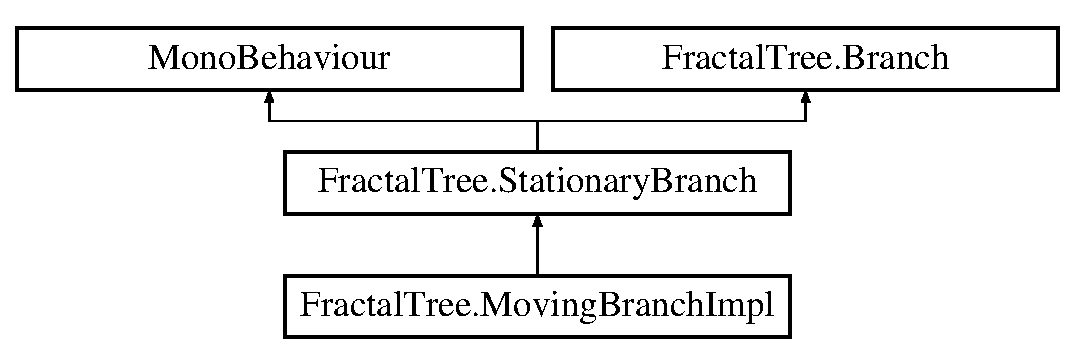
\includegraphics[height=3.000000cm]{class_fractal_tree_1_1_stationary_branch}
\end{center}
\end{figure}
\subsection*{Public Member Functions}
\begin{DoxyCompactItemize}
\item 
virtual void \hyperlink{class_fractal_tree_1_1_stationary_branch_acaa0bef74389db9f1a2f57af38557000}{Setup} (\hyperlink{interface_fractal_tree_1_1_branch}{Branch} owner, Vector2 end, float thickness, Color \hyperlink{class_fractal_tree_1_1_stationary_branch_a265ca67d50299986adb192386fc7b932}{color})
\begin{DoxyCompactList}\small\item\em Setup the specified owner, end, thickness and color. Used to create a branch that is attached to another branch. \end{DoxyCompactList}\item 
virtual void \hyperlink{class_fractal_tree_1_1_stationary_branch_a262c5810fadbd2c8aea1f2afdca57126}{Setup} (\hyperlink{interface_fractal_tree_1_1_branch}{Branch} owner, Vector2 end, float thickness, Color \hyperlink{class_fractal_tree_1_1_stationary_branch_a265ca67d50299986adb192386fc7b932}{color}, bool auto\+Mass)
\begin{DoxyCompactList}\small\item\em Setup the specified owner, end, thickness and color. Used to create a branch that is attached to another branch that has its mass autogenerated based on line width. \end{DoxyCompactList}\item 
virtual void \hyperlink{class_fractal_tree_1_1_stationary_branch_a62e1aa7062ef70a8726dfe21a9e28d76}{Setup} (Vector2 start, Vector2 end, float thickness, Color \hyperlink{class_fractal_tree_1_1_stationary_branch_a265ca67d50299986adb192386fc7b932}{color})
\begin{DoxyCompactList}\small\item\em Setup the specified owner, end, thickness and color. Used to create a branch that is attached to another branch. \end{DoxyCompactList}\item 
virtual void \hyperlink{class_fractal_tree_1_1_stationary_branch_a61cfd43bb83cf63bf1ad25f339866d7a}{Setup} (Vector2 start, Vector2 end, float thickness, Color \hyperlink{class_fractal_tree_1_1_stationary_branch_a265ca67d50299986adb192386fc7b932}{color}, bool auto\+Mass)
\begin{DoxyCompactList}\small\item\em Setup the specified owner, end, thickness and color. Used to create a branch that is attached to another branch that has its mass autogenerated based on line width. \end{DoxyCompactList}\item 
T \hyperlink{class_fractal_tree_1_1_stationary_branch_a57ff42d0c4793c0c40aa1671905bf222}{Do\+Branching$<$ T $>$} (float angle)
\begin{DoxyCompactList}\small\item\em Returns a new branch based on current branch angle plus parameter angle. \end{DoxyCompactList}\item 
void \hyperlink{class_fractal_tree_1_1_stationary_branch_a57a5b1cbc9fd081c5b8cb41b61d24502}{Do\+Colonization\+Reset} ()
\begin{DoxyCompactList}\small\item\em Resets the colonization paramater. Used only for space colonization generation. \end{DoxyCompactList}\end{DoxyCompactItemize}
\subsection*{Static Public Attributes}
\begin{DoxyCompactItemize}
\item 
static float \hyperlink{class_fractal_tree_1_1_stationary_branch_a406e104be242fe61b1c1c1ea7d67f167}{Length\+Degradation} = 0.\+67f
\begin{DoxyCompactList}\small\item\em Used by the default tree algorithm. Each branchings length is multiplied by this value. \end{DoxyCompactList}\end{DoxyCompactItemize}
\subsection*{Protected Member Functions}
\begin{DoxyCompactItemize}
\item 
\mbox{\Hypertarget{class_fractal_tree_1_1_stationary_branch_a295c6b57b1040dac71a8195a6759ec92}\label{class_fractal_tree_1_1_stationary_branch_a295c6b57b1040dac71a8195a6759ec92}} 
virtual void {\bfseries Awake} ()
\item 
void \hyperlink{class_fractal_tree_1_1_stationary_branch_a79b077e778c1d8aa92f3f4ad9a516058}{Update\+Sprite} ()
\begin{DoxyCompactList}\small\item\em Updates the sprite position, rotation, and scale in relation to the start and point. \end{DoxyCompactList}\item 
void \hyperlink{class_fractal_tree_1_1_stationary_branch_ae80389d3859645e0023dd11533b06e83}{Update\+Color} (Color \hyperlink{class_fractal_tree_1_1_stationary_branch_a265ca67d50299986adb192386fc7b932}{color})
\begin{DoxyCompactList}\small\item\em Updates the sprite renderer color. \end{DoxyCompactList}\end{DoxyCompactItemize}
\subsection*{Protected Attributes}
\begin{DoxyCompactItemize}
\item 
float \hyperlink{class_fractal_tree_1_1_stationary_branch_ad29fc34a0ab42c6bf44277d38816c568}{m\+\_\+\+Width}
\begin{DoxyCompactList}\small\item\em The width of the branch. \end{DoxyCompactList}\item 
Sprite\+Renderer \hyperlink{class_fractal_tree_1_1_stationary_branch_a395acf767c2156a0f203d00322e71512}{m\+\_\+\+Renderer}
\begin{DoxyCompactList}\small\item\em The renderer associated with the branch. \end{DoxyCompactList}\end{DoxyCompactItemize}
\subsection*{Static Protected Attributes}
\begin{DoxyCompactItemize}
\item 
static readonly float \hyperlink{class_fractal_tree_1_1_stationary_branch_aa1486b3c67665c24e3fa10eabbb30197}{S\+P\+R\+I\+T\+E\+\_\+\+S\+I\+ZE} = 100f / 100f
\begin{DoxyCompactList}\small\item\em Pixels of line sprite / pixels per units. \end{DoxyCompactList}\end{DoxyCompactItemize}
\subsection*{Properties}
\begin{DoxyCompactItemize}
\item 
Vector2 \hyperlink{class_fractal_tree_1_1_stationary_branch_a723f9bad6ef25d1b3cb215484b7a3e76}{colonization\+Dir}\hspace{0.3cm}{\ttfamily  \mbox{[}get, set\mbox{]}}
\begin{DoxyCompactList}\small\item\em Gets or sets the colonization direction. Used for space colonization tree generation. Defines the direction of the next branch in relation to nearby leaves. \end{DoxyCompactList}\item 
int \hyperlink{class_fractal_tree_1_1_stationary_branch_a8b1373ac7c9a1445f3670c6f8539b431}{colonization\+Leaf\+Count}\hspace{0.3cm}{\ttfamily  \mbox{[}get, set\mbox{]}}
\begin{DoxyCompactList}\small\item\em Gets or sets the number of nearby colonizaion leaves. \end{DoxyCompactList}\item 
virtual Vector2 \hyperlink{class_fractal_tree_1_1_stationary_branch_a536f1353b6c082d193a12efa88ed3239}{start\+Pos}\hspace{0.3cm}{\ttfamily  \mbox{[}get\mbox{]}}
\begin{DoxyCompactList}\small\item\em Gets the start position. \end{DoxyCompactList}\item 
virtual Vector2 \hyperlink{class_fractal_tree_1_1_stationary_branch_a0119dcc7bb419191c909cd1ae2f04f34}{end\+Pos}\hspace{0.3cm}{\ttfamily  \mbox{[}get\mbox{]}}
\begin{DoxyCompactList}\small\item\em Gets the end position. \end{DoxyCompactList}\item 
bool \hyperlink{class_fractal_tree_1_1_stationary_branch_aabe8c4ecdd2bcfda07911f37f171e399}{has\+Branched}\hspace{0.3cm}{\ttfamily  \mbox{[}get, set\mbox{]}}
\begin{DoxyCompactList}\small\item\em Gets or sets a value indicating whether this \hyperlink{class_fractal_tree_1_1_stationary_branch}{Fractal\+Tree.\+Stationary\+Branch} has branched. \end{DoxyCompactList}\item 
Color \hyperlink{class_fractal_tree_1_1_stationary_branch_a265ca67d50299986adb192386fc7b932}{color}\hspace{0.3cm}{\ttfamily  \mbox{[}set\mbox{]}}
\begin{DoxyCompactList}\small\item\em Sets the color of the branch sprite and updates the sprite renderer. \end{DoxyCompactList}\end{DoxyCompactItemize}


\subsection{Detailed Description}
A stationary branch. Forces cannot be applied to it. It is a line drawn onscreen by rotating and scaling a sprite between a start and end point. 



\subsection{Member Function Documentation}
\mbox{\Hypertarget{class_fractal_tree_1_1_stationary_branch_a57ff42d0c4793c0c40aa1671905bf222}\label{class_fractal_tree_1_1_stationary_branch_a57ff42d0c4793c0c40aa1671905bf222}} 
\index{Fractal\+Tree\+::\+Stationary\+Branch@{Fractal\+Tree\+::\+Stationary\+Branch}!Do\+Branching$<$ T $>$@{Do\+Branching$<$ T $>$}}
\index{Do\+Branching$<$ T $>$@{Do\+Branching$<$ T $>$}!Fractal\+Tree\+::\+Stationary\+Branch@{Fractal\+Tree\+::\+Stationary\+Branch}}
\subsubsection{\texorpdfstring{Do\+Branching$<$ T $>$()}{DoBranching< T >()}}
{\footnotesize\ttfamily T Fractal\+Tree.\+Stationary\+Branch.\+Do\+Branching$<$ T $>$ (\begin{DoxyParamCaption}\item[{float}]{angle }\end{DoxyParamCaption})}



Returns a new branch based on current branch angle plus parameter angle. 

\begin{DoxyReturn}{Returns}
The branching.
\end{DoxyReturn}

\begin{DoxyParams}{Parameters}
{\em angle} & Angle.\\
\hline
\end{DoxyParams}

\begin{DoxyTemplParams}{Template Parameters}
{\em T} & The 1st type parameter.\\
\hline
\end{DoxyTemplParams}


Implements \hyperlink{interface_fractal_tree_1_1_branch_ad3240d5e5d13df2ee22e55892f9c03cd}{Fractal\+Tree.\+Branch}.

\begin{Desc}
\item[Type Constraints]\begin{description}
\item[{\em T} : {\em Branch}]\end{description}
\end{Desc}
\mbox{\Hypertarget{class_fractal_tree_1_1_stationary_branch_a57a5b1cbc9fd081c5b8cb41b61d24502}\label{class_fractal_tree_1_1_stationary_branch_a57a5b1cbc9fd081c5b8cb41b61d24502}} 
\index{Fractal\+Tree\+::\+Stationary\+Branch@{Fractal\+Tree\+::\+Stationary\+Branch}!Do\+Colonization\+Reset@{Do\+Colonization\+Reset}}
\index{Do\+Colonization\+Reset@{Do\+Colonization\+Reset}!Fractal\+Tree\+::\+Stationary\+Branch@{Fractal\+Tree\+::\+Stationary\+Branch}}
\subsubsection{\texorpdfstring{Do\+Colonization\+Reset()}{DoColonizationReset()}}
{\footnotesize\ttfamily void Fractal\+Tree.\+Stationary\+Branch.\+Do\+Colonization\+Reset (\begin{DoxyParamCaption}{ }\end{DoxyParamCaption})}



Resets the colonization paramater. Used only for space colonization generation. 



Implements \hyperlink{interface_fractal_tree_1_1_branch_a4460379e72ec587f890b1e0cf77dbc3c}{Fractal\+Tree.\+Branch}.

\mbox{\Hypertarget{class_fractal_tree_1_1_stationary_branch_acaa0bef74389db9f1a2f57af38557000}\label{class_fractal_tree_1_1_stationary_branch_acaa0bef74389db9f1a2f57af38557000}} 
\index{Fractal\+Tree\+::\+Stationary\+Branch@{Fractal\+Tree\+::\+Stationary\+Branch}!Setup@{Setup}}
\index{Setup@{Setup}!Fractal\+Tree\+::\+Stationary\+Branch@{Fractal\+Tree\+::\+Stationary\+Branch}}
\subsubsection{\texorpdfstring{Setup()}{Setup()}\hspace{0.1cm}{\footnotesize\ttfamily [1/4]}}
{\footnotesize\ttfamily virtual void Fractal\+Tree.\+Stationary\+Branch.\+Setup (\begin{DoxyParamCaption}\item[{\hyperlink{interface_fractal_tree_1_1_branch}{Branch}}]{owner,  }\item[{Vector2}]{end,  }\item[{float}]{thickness,  }\item[{Color}]{color }\end{DoxyParamCaption})\hspace{0.3cm}{\ttfamily [virtual]}}



Setup the specified owner, end, thickness and color. Used to create a branch that is attached to another branch. 


\begin{DoxyParams}{Parameters}
{\em owner} & The attached branch.\\
\hline
{\em end} & End.\\
\hline
{\em thickness} & Thickness.\\
\hline
{\em color} & Color.\\
\hline
\end{DoxyParams}


Implements \hyperlink{interface_fractal_tree_1_1_branch_a1bad78362d67435aed4538b207f4155b}{Fractal\+Tree.\+Branch}.



Reimplemented in \hyperlink{class_fractal_tree_1_1_moving_branch_impl_a52861b34bb8a9550c6790bab90509660}{Fractal\+Tree.\+Moving\+Branch\+Impl}.

\mbox{\Hypertarget{class_fractal_tree_1_1_stationary_branch_a262c5810fadbd2c8aea1f2afdca57126}\label{class_fractal_tree_1_1_stationary_branch_a262c5810fadbd2c8aea1f2afdca57126}} 
\index{Fractal\+Tree\+::\+Stationary\+Branch@{Fractal\+Tree\+::\+Stationary\+Branch}!Setup@{Setup}}
\index{Setup@{Setup}!Fractal\+Tree\+::\+Stationary\+Branch@{Fractal\+Tree\+::\+Stationary\+Branch}}
\subsubsection{\texorpdfstring{Setup()}{Setup()}\hspace{0.1cm}{\footnotesize\ttfamily [2/4]}}
{\footnotesize\ttfamily virtual void Fractal\+Tree.\+Stationary\+Branch.\+Setup (\begin{DoxyParamCaption}\item[{\hyperlink{interface_fractal_tree_1_1_branch}{Branch}}]{owner,  }\item[{Vector2}]{end,  }\item[{float}]{thickness,  }\item[{Color}]{color,  }\item[{bool}]{auto\+Mass }\end{DoxyParamCaption})\hspace{0.3cm}{\ttfamily [virtual]}}



Setup the specified owner, end, thickness and color. Used to create a branch that is attached to another branch that has its mass autogenerated based on line width. 


\begin{DoxyParams}{Parameters}
{\em owner} & Owner.\\
\hline
{\em end} & End.\\
\hline
{\em thickness} & Thickness.\\
\hline
{\em color} & Color.\\
\hline
{\em auto\+Mass} & If set to {\ttfamily true} auto mass.\\
\hline
\end{DoxyParams}


Implements \hyperlink{interface_fractal_tree_1_1_branch_aac4a29be86256dff265190ed0d3ef250}{Fractal\+Tree.\+Branch}.



Reimplemented in \hyperlink{class_fractal_tree_1_1_moving_branch_impl_a73649451c7fbfa0793e0a1528e301215}{Fractal\+Tree.\+Moving\+Branch\+Impl}.

\mbox{\Hypertarget{class_fractal_tree_1_1_stationary_branch_a62e1aa7062ef70a8726dfe21a9e28d76}\label{class_fractal_tree_1_1_stationary_branch_a62e1aa7062ef70a8726dfe21a9e28d76}} 
\index{Fractal\+Tree\+::\+Stationary\+Branch@{Fractal\+Tree\+::\+Stationary\+Branch}!Setup@{Setup}}
\index{Setup@{Setup}!Fractal\+Tree\+::\+Stationary\+Branch@{Fractal\+Tree\+::\+Stationary\+Branch}}
\subsubsection{\texorpdfstring{Setup()}{Setup()}\hspace{0.1cm}{\footnotesize\ttfamily [3/4]}}
{\footnotesize\ttfamily virtual void Fractal\+Tree.\+Stationary\+Branch.\+Setup (\begin{DoxyParamCaption}\item[{Vector2}]{start,  }\item[{Vector2}]{end,  }\item[{float}]{thickness,  }\item[{Color}]{color }\end{DoxyParamCaption})\hspace{0.3cm}{\ttfamily [virtual]}}



Setup the specified owner, end, thickness and color. Used to create a branch that is attached to another branch. 


\begin{DoxyParams}{Parameters}
{\em owner} & The attached branch.\\
\hline
{\em end} & End.\\
\hline
{\em thickness} & Thickness.\\
\hline
{\em color} & Color.\\
\hline
{\em start} & Start.\\
\hline
\end{DoxyParams}


Implements \hyperlink{interface_fractal_tree_1_1_branch_a6c313c988c603a9d558871bd560a0b70}{Fractal\+Tree.\+Branch}.



Reimplemented in \hyperlink{class_fractal_tree_1_1_moving_branch_impl_aeea52b05117e613e0dd6c9ee5fbafb58}{Fractal\+Tree.\+Moving\+Branch\+Impl}.

\mbox{\Hypertarget{class_fractal_tree_1_1_stationary_branch_a61cfd43bb83cf63bf1ad25f339866d7a}\label{class_fractal_tree_1_1_stationary_branch_a61cfd43bb83cf63bf1ad25f339866d7a}} 
\index{Fractal\+Tree\+::\+Stationary\+Branch@{Fractal\+Tree\+::\+Stationary\+Branch}!Setup@{Setup}}
\index{Setup@{Setup}!Fractal\+Tree\+::\+Stationary\+Branch@{Fractal\+Tree\+::\+Stationary\+Branch}}
\subsubsection{\texorpdfstring{Setup()}{Setup()}\hspace{0.1cm}{\footnotesize\ttfamily [4/4]}}
{\footnotesize\ttfamily virtual void Fractal\+Tree.\+Stationary\+Branch.\+Setup (\begin{DoxyParamCaption}\item[{Vector2}]{start,  }\item[{Vector2}]{end,  }\item[{float}]{thickness,  }\item[{Color}]{color,  }\item[{bool}]{auto\+Mass }\end{DoxyParamCaption})\hspace{0.3cm}{\ttfamily [virtual]}}



Setup the specified owner, end, thickness and color. Used to create a branch that is attached to another branch that has its mass autogenerated based on line width. 


\begin{DoxyParams}{Parameters}
{\em owner} & Owner.\\
\hline
{\em end} & End.\\
\hline
{\em thickness} & Thickness.\\
\hline
{\em color} & Color.\\
\hline
{\em start} & Start.\\
\hline
{\em auto\+Mass} & If set to {\ttfamily true} auto mass.\\
\hline
\end{DoxyParams}


Implements \hyperlink{interface_fractal_tree_1_1_branch_ad813c22ae887cf465056d5eee5acb651}{Fractal\+Tree.\+Branch}.



Reimplemented in \hyperlink{class_fractal_tree_1_1_moving_branch_impl_a4e7cde65899abaf121a906d06874c330}{Fractal\+Tree.\+Moving\+Branch\+Impl}.

\mbox{\Hypertarget{class_fractal_tree_1_1_stationary_branch_ae80389d3859645e0023dd11533b06e83}\label{class_fractal_tree_1_1_stationary_branch_ae80389d3859645e0023dd11533b06e83}} 
\index{Fractal\+Tree\+::\+Stationary\+Branch@{Fractal\+Tree\+::\+Stationary\+Branch}!Update\+Color@{Update\+Color}}
\index{Update\+Color@{Update\+Color}!Fractal\+Tree\+::\+Stationary\+Branch@{Fractal\+Tree\+::\+Stationary\+Branch}}
\subsubsection{\texorpdfstring{Update\+Color()}{UpdateColor()}}
{\footnotesize\ttfamily void Fractal\+Tree.\+Stationary\+Branch.\+Update\+Color (\begin{DoxyParamCaption}\item[{Color}]{color }\end{DoxyParamCaption})\hspace{0.3cm}{\ttfamily [protected]}}



Updates the sprite renderer color. 


\begin{DoxyParams}{Parameters}
{\em color} & Color.\\
\hline
\end{DoxyParams}
\mbox{\Hypertarget{class_fractal_tree_1_1_stationary_branch_a79b077e778c1d8aa92f3f4ad9a516058}\label{class_fractal_tree_1_1_stationary_branch_a79b077e778c1d8aa92f3f4ad9a516058}} 
\index{Fractal\+Tree\+::\+Stationary\+Branch@{Fractal\+Tree\+::\+Stationary\+Branch}!Update\+Sprite@{Update\+Sprite}}
\index{Update\+Sprite@{Update\+Sprite}!Fractal\+Tree\+::\+Stationary\+Branch@{Fractal\+Tree\+::\+Stationary\+Branch}}
\subsubsection{\texorpdfstring{Update\+Sprite()}{UpdateSprite()}}
{\footnotesize\ttfamily void Fractal\+Tree.\+Stationary\+Branch.\+Update\+Sprite (\begin{DoxyParamCaption}{ }\end{DoxyParamCaption})\hspace{0.3cm}{\ttfamily [protected]}}



Updates the sprite position, rotation, and scale in relation to the start and point. 



\subsection{Member Data Documentation}
\mbox{\Hypertarget{class_fractal_tree_1_1_stationary_branch_a406e104be242fe61b1c1c1ea7d67f167}\label{class_fractal_tree_1_1_stationary_branch_a406e104be242fe61b1c1c1ea7d67f167}} 
\index{Fractal\+Tree\+::\+Stationary\+Branch@{Fractal\+Tree\+::\+Stationary\+Branch}!Length\+Degradation@{Length\+Degradation}}
\index{Length\+Degradation@{Length\+Degradation}!Fractal\+Tree\+::\+Stationary\+Branch@{Fractal\+Tree\+::\+Stationary\+Branch}}
\subsubsection{\texorpdfstring{Length\+Degradation}{LengthDegradation}}
{\footnotesize\ttfamily float Fractal\+Tree.\+Stationary\+Branch.\+Length\+Degradation = 0.\+67f\hspace{0.3cm}{\ttfamily [static]}}



Used by the default tree algorithm. Each branchings length is multiplied by this value. 

\mbox{\Hypertarget{class_fractal_tree_1_1_stationary_branch_a395acf767c2156a0f203d00322e71512}\label{class_fractal_tree_1_1_stationary_branch_a395acf767c2156a0f203d00322e71512}} 
\index{Fractal\+Tree\+::\+Stationary\+Branch@{Fractal\+Tree\+::\+Stationary\+Branch}!m\+\_\+\+Renderer@{m\+\_\+\+Renderer}}
\index{m\+\_\+\+Renderer@{m\+\_\+\+Renderer}!Fractal\+Tree\+::\+Stationary\+Branch@{Fractal\+Tree\+::\+Stationary\+Branch}}
\subsubsection{\texorpdfstring{m\+\_\+\+Renderer}{m\_Renderer}}
{\footnotesize\ttfamily Sprite\+Renderer Fractal\+Tree.\+Stationary\+Branch.\+m\+\_\+\+Renderer\hspace{0.3cm}{\ttfamily [protected]}}



The renderer associated with the branch. 

\mbox{\Hypertarget{class_fractal_tree_1_1_stationary_branch_ad29fc34a0ab42c6bf44277d38816c568}\label{class_fractal_tree_1_1_stationary_branch_ad29fc34a0ab42c6bf44277d38816c568}} 
\index{Fractal\+Tree\+::\+Stationary\+Branch@{Fractal\+Tree\+::\+Stationary\+Branch}!m\+\_\+\+Width@{m\+\_\+\+Width}}
\index{m\+\_\+\+Width@{m\+\_\+\+Width}!Fractal\+Tree\+::\+Stationary\+Branch@{Fractal\+Tree\+::\+Stationary\+Branch}}
\subsubsection{\texorpdfstring{m\+\_\+\+Width}{m\_Width}}
{\footnotesize\ttfamily float Fractal\+Tree.\+Stationary\+Branch.\+m\+\_\+\+Width\hspace{0.3cm}{\ttfamily [protected]}}



The width of the branch. 

\mbox{\Hypertarget{class_fractal_tree_1_1_stationary_branch_aa1486b3c67665c24e3fa10eabbb30197}\label{class_fractal_tree_1_1_stationary_branch_aa1486b3c67665c24e3fa10eabbb30197}} 
\index{Fractal\+Tree\+::\+Stationary\+Branch@{Fractal\+Tree\+::\+Stationary\+Branch}!S\+P\+R\+I\+T\+E\+\_\+\+S\+I\+ZE@{S\+P\+R\+I\+T\+E\+\_\+\+S\+I\+ZE}}
\index{S\+P\+R\+I\+T\+E\+\_\+\+S\+I\+ZE@{S\+P\+R\+I\+T\+E\+\_\+\+S\+I\+ZE}!Fractal\+Tree\+::\+Stationary\+Branch@{Fractal\+Tree\+::\+Stationary\+Branch}}
\subsubsection{\texorpdfstring{S\+P\+R\+I\+T\+E\+\_\+\+S\+I\+ZE}{SPRITE\_SIZE}}
{\footnotesize\ttfamily readonly float Fractal\+Tree.\+Stationary\+Branch.\+S\+P\+R\+I\+T\+E\+\_\+\+S\+I\+ZE = 100f / 100f\hspace{0.3cm}{\ttfamily [static]}, {\ttfamily [protected]}}



Pixels of line sprite / pixels per units. 



\subsection{Property Documentation}
\mbox{\Hypertarget{class_fractal_tree_1_1_stationary_branch_a723f9bad6ef25d1b3cb215484b7a3e76}\label{class_fractal_tree_1_1_stationary_branch_a723f9bad6ef25d1b3cb215484b7a3e76}} 
\index{Fractal\+Tree\+::\+Stationary\+Branch@{Fractal\+Tree\+::\+Stationary\+Branch}!colonization\+Dir@{colonization\+Dir}}
\index{colonization\+Dir@{colonization\+Dir}!Fractal\+Tree\+::\+Stationary\+Branch@{Fractal\+Tree\+::\+Stationary\+Branch}}
\subsubsection{\texorpdfstring{colonization\+Dir}{colonizationDir}}
{\footnotesize\ttfamily Vector2 Fractal\+Tree.\+Stationary\+Branch.\+colonization\+Dir\hspace{0.3cm}{\ttfamily [get]}, {\ttfamily [set]}}



Gets or sets the colonization direction. Used for space colonization tree generation. Defines the direction of the next branch in relation to nearby leaves. 

The colonization dir.\mbox{\Hypertarget{class_fractal_tree_1_1_stationary_branch_a8b1373ac7c9a1445f3670c6f8539b431}\label{class_fractal_tree_1_1_stationary_branch_a8b1373ac7c9a1445f3670c6f8539b431}} 
\index{Fractal\+Tree\+::\+Stationary\+Branch@{Fractal\+Tree\+::\+Stationary\+Branch}!colonization\+Leaf\+Count@{colonization\+Leaf\+Count}}
\index{colonization\+Leaf\+Count@{colonization\+Leaf\+Count}!Fractal\+Tree\+::\+Stationary\+Branch@{Fractal\+Tree\+::\+Stationary\+Branch}}
\subsubsection{\texorpdfstring{colonization\+Leaf\+Count}{colonizationLeafCount}}
{\footnotesize\ttfamily int Fractal\+Tree.\+Stationary\+Branch.\+colonization\+Leaf\+Count\hspace{0.3cm}{\ttfamily [get]}, {\ttfamily [set]}}



Gets or sets the number of nearby colonizaion leaves. 

The colonization leaf count.\mbox{\Hypertarget{class_fractal_tree_1_1_stationary_branch_a265ca67d50299986adb192386fc7b932}\label{class_fractal_tree_1_1_stationary_branch_a265ca67d50299986adb192386fc7b932}} 
\index{Fractal\+Tree\+::\+Stationary\+Branch@{Fractal\+Tree\+::\+Stationary\+Branch}!color@{color}}
\index{color@{color}!Fractal\+Tree\+::\+Stationary\+Branch@{Fractal\+Tree\+::\+Stationary\+Branch}}
\subsubsection{\texorpdfstring{color}{color}}
{\footnotesize\ttfamily Color Fractal\+Tree.\+Stationary\+Branch.\+color\hspace{0.3cm}{\ttfamily [set]}}



Sets the color of the branch sprite and updates the sprite renderer. 

The color.\mbox{\Hypertarget{class_fractal_tree_1_1_stationary_branch_a0119dcc7bb419191c909cd1ae2f04f34}\label{class_fractal_tree_1_1_stationary_branch_a0119dcc7bb419191c909cd1ae2f04f34}} 
\index{Fractal\+Tree\+::\+Stationary\+Branch@{Fractal\+Tree\+::\+Stationary\+Branch}!end\+Pos@{end\+Pos}}
\index{end\+Pos@{end\+Pos}!Fractal\+Tree\+::\+Stationary\+Branch@{Fractal\+Tree\+::\+Stationary\+Branch}}
\subsubsection{\texorpdfstring{end\+Pos}{endPos}}
{\footnotesize\ttfamily virtual Vector2 Fractal\+Tree.\+Stationary\+Branch.\+end\+Pos\hspace{0.3cm}{\ttfamily [get]}}



Gets the end position. 

The end position.\mbox{\Hypertarget{class_fractal_tree_1_1_stationary_branch_aabe8c4ecdd2bcfda07911f37f171e399}\label{class_fractal_tree_1_1_stationary_branch_aabe8c4ecdd2bcfda07911f37f171e399}} 
\index{Fractal\+Tree\+::\+Stationary\+Branch@{Fractal\+Tree\+::\+Stationary\+Branch}!has\+Branched@{has\+Branched}}
\index{has\+Branched@{has\+Branched}!Fractal\+Tree\+::\+Stationary\+Branch@{Fractal\+Tree\+::\+Stationary\+Branch}}
\subsubsection{\texorpdfstring{has\+Branched}{hasBranched}}
{\footnotesize\ttfamily bool Fractal\+Tree.\+Stationary\+Branch.\+has\+Branched\hspace{0.3cm}{\ttfamily [get]}, {\ttfamily [set]}}



Gets or sets a value indicating whether this \hyperlink{class_fractal_tree_1_1_stationary_branch}{Fractal\+Tree.\+Stationary\+Branch} has branched. 

{\ttfamily true} if has branched; otherwise, {\ttfamily false}.\mbox{\Hypertarget{class_fractal_tree_1_1_stationary_branch_a536f1353b6c082d193a12efa88ed3239}\label{class_fractal_tree_1_1_stationary_branch_a536f1353b6c082d193a12efa88ed3239}} 
\index{Fractal\+Tree\+::\+Stationary\+Branch@{Fractal\+Tree\+::\+Stationary\+Branch}!start\+Pos@{start\+Pos}}
\index{start\+Pos@{start\+Pos}!Fractal\+Tree\+::\+Stationary\+Branch@{Fractal\+Tree\+::\+Stationary\+Branch}}
\subsubsection{\texorpdfstring{start\+Pos}{startPos}}
{\footnotesize\ttfamily virtual Vector2 Fractal\+Tree.\+Stationary\+Branch.\+start\+Pos\hspace{0.3cm}{\ttfamily [get]}}



Gets the start position. 

The start position.

The documentation for this class was generated from the following file\+:\begin{DoxyCompactItemize}
\item 
F\+T/\+Scripts/\+Branch/Stationary\+Branch.\+cs\end{DoxyCompactItemize}

\hypertarget{class_fractal_tree_1_1_stationary_tree_builder}{}\section{Fractal\+Tree.\+Stationary\+Tree\+Builder Class Reference}
\label{class_fractal_tree_1_1_stationary_tree_builder}\index{Fractal\+Tree.\+Stationary\+Tree\+Builder@{Fractal\+Tree.\+Stationary\+Tree\+Builder}}


Builds a stationary tree.  


Inheritance diagram for Fractal\+Tree.\+Stationary\+Tree\+Builder\+:\begin{figure}[H]
\begin{center}
\leavevmode
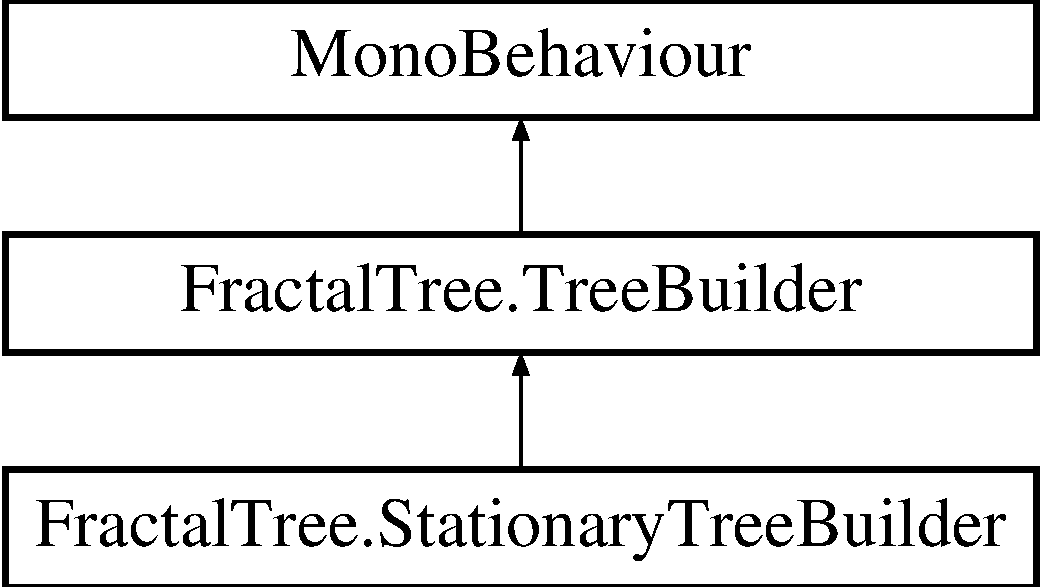
\includegraphics[height=3.000000cm]{class_fractal_tree_1_1_stationary_tree_builder}
\end{center}
\end{figure}
\subsection*{Public Member Functions}
\begin{DoxyCompactItemize}
\item 
override void \hyperlink{class_fractal_tree_1_1_stationary_tree_builder_ab11cfafdc3a0e6c29fe4eef3318331b7}{Build} ()
\begin{DoxyCompactList}\small\item\em Build this instance. \end{DoxyCompactList}\item 
override void \hyperlink{class_fractal_tree_1_1_stationary_tree_builder_a6f7254b5a4ef6ebbdd88abadfc221b4c}{Remove} ()
\begin{DoxyCompactList}\small\item\em Deletes all child branches and clears branch list. \end{DoxyCompactList}\end{DoxyCompactItemize}
\subsection*{Properties}
\begin{DoxyCompactItemize}
\item 
List$<$ \hyperlink{interface_fractal_tree_1_1_branch}{Branch} $>$ \hyperlink{class_fractal_tree_1_1_stationary_tree_builder_a103e903dbfba82226ab6cbb08fff382a}{branches}\hspace{0.3cm}{\ttfamily  \mbox{[}get\mbox{]}}
\begin{DoxyCompactList}\small\item\em A list of all branches associated with the tree. \end{DoxyCompactList}\end{DoxyCompactItemize}
\subsection*{Additional Inherited Members}


\subsection{Detailed Description}
Builds a stationary tree. 



\subsection{Member Function Documentation}
\mbox{\Hypertarget{class_fractal_tree_1_1_stationary_tree_builder_ab11cfafdc3a0e6c29fe4eef3318331b7}\label{class_fractal_tree_1_1_stationary_tree_builder_ab11cfafdc3a0e6c29fe4eef3318331b7}} 
\index{Fractal\+Tree\+::\+Stationary\+Tree\+Builder@{Fractal\+Tree\+::\+Stationary\+Tree\+Builder}!Build@{Build}}
\index{Build@{Build}!Fractal\+Tree\+::\+Stationary\+Tree\+Builder@{Fractal\+Tree\+::\+Stationary\+Tree\+Builder}}
\subsubsection{\texorpdfstring{Build()}{Build()}}
{\footnotesize\ttfamily override void Fractal\+Tree.\+Stationary\+Tree\+Builder.\+Build (\begin{DoxyParamCaption}{ }\end{DoxyParamCaption})\hspace{0.3cm}{\ttfamily [virtual]}}



Build this instance. 



Implements \hyperlink{class_fractal_tree_1_1_tree_builder}{Fractal\+Tree.\+Tree\+Builder}.

\mbox{\Hypertarget{class_fractal_tree_1_1_stationary_tree_builder_a6f7254b5a4ef6ebbdd88abadfc221b4c}\label{class_fractal_tree_1_1_stationary_tree_builder_a6f7254b5a4ef6ebbdd88abadfc221b4c}} 
\index{Fractal\+Tree\+::\+Stationary\+Tree\+Builder@{Fractal\+Tree\+::\+Stationary\+Tree\+Builder}!Remove@{Remove}}
\index{Remove@{Remove}!Fractal\+Tree\+::\+Stationary\+Tree\+Builder@{Fractal\+Tree\+::\+Stationary\+Tree\+Builder}}
\subsubsection{\texorpdfstring{Remove()}{Remove()}}
{\footnotesize\ttfamily override void Fractal\+Tree.\+Stationary\+Tree\+Builder.\+Remove (\begin{DoxyParamCaption}{ }\end{DoxyParamCaption})\hspace{0.3cm}{\ttfamily [virtual]}}



Deletes all child branches and clears branch list. 



Implements \hyperlink{class_fractal_tree_1_1_tree_builder}{Fractal\+Tree.\+Tree\+Builder}.



\subsection{Property Documentation}
\mbox{\Hypertarget{class_fractal_tree_1_1_stationary_tree_builder_a103e903dbfba82226ab6cbb08fff382a}\label{class_fractal_tree_1_1_stationary_tree_builder_a103e903dbfba82226ab6cbb08fff382a}} 
\index{Fractal\+Tree\+::\+Stationary\+Tree\+Builder@{Fractal\+Tree\+::\+Stationary\+Tree\+Builder}!branches@{branches}}
\index{branches@{branches}!Fractal\+Tree\+::\+Stationary\+Tree\+Builder@{Fractal\+Tree\+::\+Stationary\+Tree\+Builder}}
\subsubsection{\texorpdfstring{branches}{branches}}
{\footnotesize\ttfamily List$<$\hyperlink{interface_fractal_tree_1_1_branch}{Branch}$>$ Fractal\+Tree.\+Stationary\+Tree\+Builder.\+branches\hspace{0.3cm}{\ttfamily [get]}}



A list of all branches associated with the tree. 

The branches.

The documentation for this class was generated from the following file\+:\begin{DoxyCompactItemize}
\item 
F\+T/\+Scripts/\+Tree Builders/Stationary\+Tree\+Builder.\+cs\end{DoxyCompactItemize}

\hypertarget{class_fractal_tree_1_1_stationary_tree_builder_editor}{}\section{Fractal\+Tree.\+Stationary\+Tree\+Builder\+Editor Class Reference}
\label{class_fractal_tree_1_1_stationary_tree_builder_editor}\index{Fractal\+Tree.\+Stationary\+Tree\+Builder\+Editor@{Fractal\+Tree.\+Stationary\+Tree\+Builder\+Editor}}
Inheritance diagram for Fractal\+Tree.\+Stationary\+Tree\+Builder\+Editor\+:\begin{figure}[H]
\begin{center}
\leavevmode
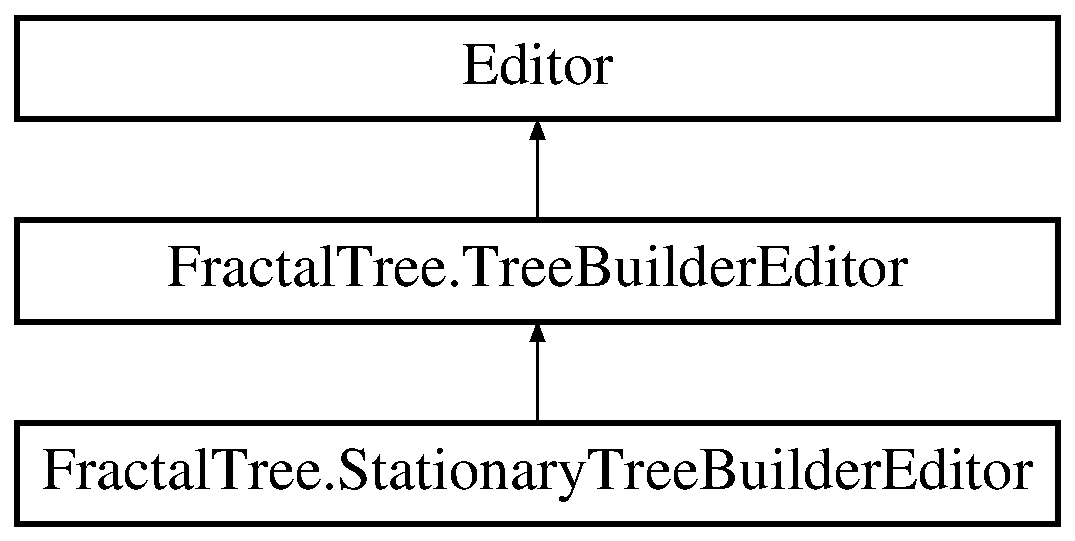
\includegraphics[height=3.000000cm]{class_fractal_tree_1_1_stationary_tree_builder_editor}
\end{center}
\end{figure}
\subsection*{Public Member Functions}
\begin{DoxyCompactItemize}
\item 
\mbox{\Hypertarget{class_fractal_tree_1_1_stationary_tree_builder_editor_a8a98e0bcfbd7f645a7aa4ef051cfb404}\label{class_fractal_tree_1_1_stationary_tree_builder_editor_a8a98e0bcfbd7f645a7aa4ef051cfb404}} 
override void {\bfseries On\+Inspector\+G\+UI} ()
\end{DoxyCompactItemize}
\subsection*{Additional Inherited Members}


The documentation for this class was generated from the following file\+:\begin{DoxyCompactItemize}
\item 
F\+T/\+Scripts/\+Editor/Stationary\+Tree\+Builder\+Editor.\+cs\end{DoxyCompactItemize}

\hypertarget{interface_fractal_tree_1_1_tree}{}\section{Fractal\+Tree.\+Tree Interface Reference}
\label{interface_fractal_tree_1_1_tree}\index{Fractal\+Tree.\+Tree@{Fractal\+Tree.\+Tree}}
Inheritance diagram for Fractal\+Tree.\+Tree\+:\begin{figure}[H]
\begin{center}
\leavevmode
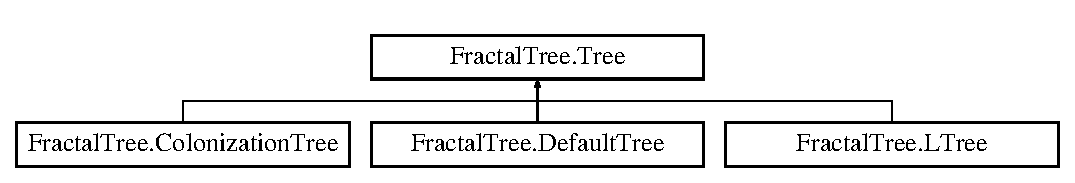
\includegraphics[height=2.000000cm]{interface_fractal_tree_1_1_tree}
\end{center}
\end{figure}
\subsection*{Public Member Functions}
\begin{DoxyCompactItemize}
\item 
\hypertarget{interface_fractal_tree_1_1_tree_a63c5353759447db5034d7ee1c83fbd78}{}\label{interface_fractal_tree_1_1_tree_a63c5353759447db5034d7ee1c83fbd78} 
List$<$ T $>$ {\bfseries Generate$<$ T $>$} ()
\end{DoxyCompactItemize}


The documentation for this interface was generated from the following file\+:\begin{DoxyCompactItemize}
\item 
Moving\+Tree\+Builder.\+cs\end{DoxyCompactItemize}

\hypertarget{class_fractal_tree_1_1_tree_builder}{}\section{Fractal\+Tree.\+Tree\+Builder Class Reference}
\label{class_fractal_tree_1_1_tree_builder}\index{Fractal\+Tree.\+Tree\+Builder@{Fractal\+Tree.\+Tree\+Builder}}


The base tree builder class. Provides paramaters for default, L, and colonization tree generation.  


Inheritance diagram for Fractal\+Tree.\+Tree\+Builder\+:\begin{figure}[H]
\begin{center}
\leavevmode
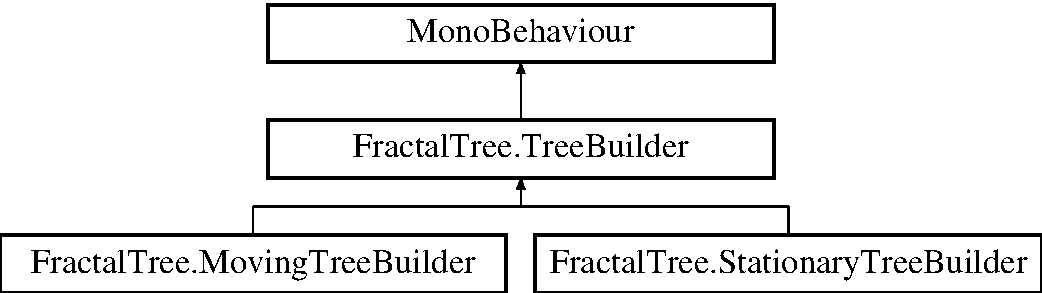
\includegraphics[height=3.000000cm]{class_fractal_tree_1_1_tree_builder}
\end{center}
\end{figure}
\subsection*{Public Types}
\begin{DoxyCompactItemize}
\item 
enum \hyperlink{class_fractal_tree_1_1_tree_builder_a955d67cfa976440cc427e591be74f979}{Tree\+Type} \{ {\bfseries Branching}, 
{\bfseries L\+Tree}, 
{\bfseries Colonization}
 \}\begin{DoxyCompactList}\small\item\em \hyperlink{interface_fractal_tree_1_1_tree}{Tree} type. \end{DoxyCompactList}
\end{DoxyCompactItemize}
\subsection*{Public Member Functions}
\begin{DoxyCompactItemize}
\item 
\mbox{\Hypertarget{class_fractal_tree_1_1_tree_builder_a88adcd333ec7886c37d9810eab7fb8f0}\label{class_fractal_tree_1_1_tree_builder_a88adcd333ec7886c37d9810eab7fb8f0}} 
abstract void {\bfseries Build} ()
\item 
\mbox{\Hypertarget{class_fractal_tree_1_1_tree_builder_a78e204c24a9e5e49734ecaa87d395e53}\label{class_fractal_tree_1_1_tree_builder_a78e204c24a9e5e49734ecaa87d395e53}} 
abstract void {\bfseries Remove} ()
\end{DoxyCompactItemize}
\subsection*{Public Attributes}
\begin{DoxyCompactItemize}
\item 
bool \hyperlink{class_fractal_tree_1_1_tree_builder_a430c3374fd2e1302f232d08bca9558b2}{build\+On\+Start} = true
\begin{DoxyCompactList}\small\item\em If true, builds tree on start. \end{DoxyCompactList}\item 
\hyperlink{class_fractal_tree_1_1_tree_builder_a955d67cfa976440cc427e591be74f979}{Tree\+Type} \hyperlink{class_fractal_tree_1_1_tree_builder_aa2f66ebffbf59d18232884f85e95490d}{tree\+Type} = Tree\+Type.\+Branching
\begin{DoxyCompactList}\small\item\em The tree type to generate. \end{DoxyCompactList}\item 
Game\+Object \hyperlink{class_fractal_tree_1_1_tree_builder_a3cc99e5fd404b3916dc29f5dc5223d8c}{branch\+Prefab}
\begin{DoxyCompactList}\small\item\em The branch prefab. If tree to generate is moving then prefab should have \hyperlink{interface_fractal_tree_1_1_moving_branch}{Moving\+Branch} script attached. \end{DoxyCompactList}\item 
Color \hyperlink{class_fractal_tree_1_1_tree_builder_a5277c397ded85184011c9ccda8f83563}{default\+Branch\+Colour} = Color.\+white
\begin{DoxyCompactList}\small\item\em The branch colour for the default tree. \end{DoxyCompactList}\item 
int \hyperlink{class_fractal_tree_1_1_tree_builder_a6f7229c6652a8d52f4227f5e7dce3123}{default\+Growth\+Count} = 8
\begin{DoxyCompactList}\small\item\em The number of tree generations. \end{DoxyCompactList}\item 
float \hyperlink{class_fractal_tree_1_1_tree_builder_a34195cdf1a552ee1027bfbf42682ea29}{default\+Initial\+Length} = 5f
\begin{DoxyCompactList}\small\item\em The default length of the initial branches for the default tree generation. \end{DoxyCompactList}\item 
float \hyperlink{class_fractal_tree_1_1_tree_builder_a002013c39a026974af2745840d7784bd}{default\+Length\+Reduction\+On\+New\+Generation} = 0.\+67f
\begin{DoxyCompactList}\small\item\em The length degradation for the default tree. Branches are reduced in size by this factor. \end{DoxyCompactList}\item 
float \hyperlink{class_fractal_tree_1_1_tree_builder_a71036891662e482caeb410dadd5bfe65}{default\+Angle} = 45f
\begin{DoxyCompactList}\small\item\em The angle for default tree branching. \end{DoxyCompactList}\item 
float \hyperlink{class_fractal_tree_1_1_tree_builder_a1f60a72d865f9cca5bb155a72ff5f6ef}{default\+Width} = 0.\+04f
\begin{DoxyCompactList}\small\item\em The width of the branches for the default tree generator. \end{DoxyCompactList}\item 
bool \hyperlink{class_fractal_tree_1_1_tree_builder_acc1a7487b339290c552ef136fec40b02}{l\+Tree\+Auto\+Width} = true
\begin{DoxyCompactList}\small\item\em When true, the width of the branches will be set automatically based on the colours. \end{DoxyCompactList}\item 
bool \hyperlink{class_fractal_tree_1_1_tree_builder_a4ba732b60fd74e4db9f5422a7e9ffd82}{l\+Tree\+Mass\+Based\+On\+Width} = true
\begin{DoxyCompactList}\small\item\em When true, the mass of the branches will be set automatically based on colours. Used only when generating a moving tree. \end{DoxyCompactList}\item 
float \hyperlink{class_fractal_tree_1_1_tree_builder_a382d4bba4cac7e05681e75109801dd92}{l\+Tree\+Width} = 0.\+03f
\begin{DoxyCompactList}\small\item\em The max branch width for L trees. \end{DoxyCompactList}\item 
int \hyperlink{class_fractal_tree_1_1_tree_builder_af50b64e86abfc4709fdfc6368ff7504b}{l\+Tree\+Growth\+Count} = 5
\begin{DoxyCompactList}\small\item\em The number of L tree generations. \end{DoxyCompactList}\item 
string \hyperlink{class_fractal_tree_1_1_tree_builder_a0ed6efbc756277236c9b209ebcba829a}{l\+Tree\+Axiom} = \char`\"{}FX\char`\"{}
\begin{DoxyCompactList}\small\item\em The l tree axiom. The initial seed used to generate a L tree. \end{DoxyCompactList}\item 
\hyperlink{class_fractal_tree_1_1_l_rule}{L\+Rule} \mbox{[}$\,$\mbox{]} \hyperlink{class_fractal_tree_1_1_tree_builder_a725a1ff0ebe0fbbc78e22eedea80a50e}{l\+Tree\+Rules}
\begin{DoxyCompactList}\small\item\em The rules applied to the axoim. \end{DoxyCompactList}\item 
float \hyperlink{class_fractal_tree_1_1_tree_builder_a7416e2e2bea136c1406f79a98a8026ee}{l\+Tree\+Branch\+Length} = 0.\+17f
\begin{DoxyCompactList}\small\item\em The length of the l tree branch. \end{DoxyCompactList}\item 
float \hyperlink{class_fractal_tree_1_1_tree_builder_a10a0d2b7b57b98c4232ba414cdfa8436}{l\+Tree\+Angle} = 25f
\begin{DoxyCompactList}\small\item\em The angles used to branch an L tree. \end{DoxyCompactList}\item 
Color \mbox{[}$\,$\mbox{]} \hyperlink{class_fractal_tree_1_1_tree_builder_adf9df8010eaa8ed629b6e5210474b7eb}{l\+Tree\+Colours}
\begin{DoxyCompactList}\small\item\em The L tree colours. \end{DoxyCompactList}\item 
Transform \hyperlink{class_fractal_tree_1_1_tree_builder_a17c8e9ca6955ef3d2eadbf0fc54acfa3}{colonization\+Leaf\+Parent}
\begin{DoxyCompactList}\small\item\em The parent of the game object that holds the colonization leaves. \end{DoxyCompactList}\item 
\mbox{\Hypertarget{class_fractal_tree_1_1_tree_builder_ad49cb5210ad4c146bfb44a2c04f47f36}\label{class_fractal_tree_1_1_tree_builder_ad49cb5210ad4c146bfb44a2c04f47f36}} 
Color {\bfseries colonization\+Branch\+Color} = Color.\+white
\item 
float \hyperlink{class_fractal_tree_1_1_tree_builder_a1cd91a1a14415505680fa2deae9468ca}{colonization\+Initial\+Length} = 1f
\begin{DoxyCompactList}\small\item\em The initial length for a colonization tree trunk. \end{DoxyCompactList}\item 
float \hyperlink{class_fractal_tree_1_1_tree_builder_a22b8c477430d16faa020d724c8573a57}{colonization\+Width} = 0.\+04f
\begin{DoxyCompactList}\small\item\em The width of the colonization tree branches. \end{DoxyCompactList}\item 
float \hyperlink{class_fractal_tree_1_1_tree_builder_ac7abe13cc887bafe266773e33513d69a}{colonization\+Min\+Distance} = 1f
\begin{DoxyCompactList}\small\item\em The minimum distance between the branch and a colonization leaf for it to be registered. \end{DoxyCompactList}\item 
float \hyperlink{class_fractal_tree_1_1_tree_builder_a21cbebdabadaf5d205a038d20db2f702}{colonization\+Max\+Distance} = 10f
\begin{DoxyCompactList}\small\item\em The maximum distance between the branch and a colonization leaf for it to be registered. \end{DoxyCompactList}\end{DoxyCompactItemize}
\subsection*{Protected Member Functions}
\begin{DoxyCompactItemize}
\item 
List$<$ T $>$ \hyperlink{class_fractal_tree_1_1_tree_builder_aa2d0ae2616577e6c0cdf7e68cdf4dffb}{Do\+Build$<$ T $>$} ()
\begin{DoxyCompactList}\small\item\em Build this instance of the tree. \end{DoxyCompactList}\item 
\hyperlink{interface_fractal_tree_1_1_tree}{Tree} \hyperlink{class_fractal_tree_1_1_tree_builder_a8bea11ef52d57a75292efd34e6f40779}{Create\+Tree} ()
\begin{DoxyCompactList}\small\item\em Creates a tree based on tree\+Type. \end{DoxyCompactList}\end{DoxyCompactItemize}


\subsection{Detailed Description}
The base tree builder class. Provides paramaters for default, L, and colonization tree generation. 



\subsection{Member Enumeration Documentation}
\mbox{\Hypertarget{class_fractal_tree_1_1_tree_builder_a955d67cfa976440cc427e591be74f979}\label{class_fractal_tree_1_1_tree_builder_a955d67cfa976440cc427e591be74f979}} 
\index{Fractal\+Tree\+::\+Tree\+Builder@{Fractal\+Tree\+::\+Tree\+Builder}!Tree\+Type@{Tree\+Type}}
\index{Tree\+Type@{Tree\+Type}!Fractal\+Tree\+::\+Tree\+Builder@{Fractal\+Tree\+::\+Tree\+Builder}}
\subsubsection{\texorpdfstring{Tree\+Type}{TreeType}}
{\footnotesize\ttfamily enum \hyperlink{class_fractal_tree_1_1_tree_builder_a955d67cfa976440cc427e591be74f979}{Fractal\+Tree.\+Tree\+Builder.\+Tree\+Type}\hspace{0.3cm}{\ttfamily [strong]}}



\hyperlink{interface_fractal_tree_1_1_tree}{Tree} type. 



\subsection{Member Function Documentation}
\mbox{\Hypertarget{class_fractal_tree_1_1_tree_builder_a8bea11ef52d57a75292efd34e6f40779}\label{class_fractal_tree_1_1_tree_builder_a8bea11ef52d57a75292efd34e6f40779}} 
\index{Fractal\+Tree\+::\+Tree\+Builder@{Fractal\+Tree\+::\+Tree\+Builder}!Create\+Tree@{Create\+Tree}}
\index{Create\+Tree@{Create\+Tree}!Fractal\+Tree\+::\+Tree\+Builder@{Fractal\+Tree\+::\+Tree\+Builder}}
\subsubsection{\texorpdfstring{Create\+Tree()}{CreateTree()}}
{\footnotesize\ttfamily \hyperlink{interface_fractal_tree_1_1_tree}{Tree} Fractal\+Tree.\+Tree\+Builder.\+Create\+Tree (\begin{DoxyParamCaption}{ }\end{DoxyParamCaption})\hspace{0.3cm}{\ttfamily [protected]}}



Creates a tree based on tree\+Type. 

\begin{DoxyReturn}{Returns}
The tree.
\end{DoxyReturn}
\mbox{\Hypertarget{class_fractal_tree_1_1_tree_builder_aa2d0ae2616577e6c0cdf7e68cdf4dffb}\label{class_fractal_tree_1_1_tree_builder_aa2d0ae2616577e6c0cdf7e68cdf4dffb}} 
\index{Fractal\+Tree\+::\+Tree\+Builder@{Fractal\+Tree\+::\+Tree\+Builder}!Do\+Build$<$ T $>$@{Do\+Build$<$ T $>$}}
\index{Do\+Build$<$ T $>$@{Do\+Build$<$ T $>$}!Fractal\+Tree\+::\+Tree\+Builder@{Fractal\+Tree\+::\+Tree\+Builder}}
\subsubsection{\texorpdfstring{Do\+Build$<$ T $>$()}{DoBuild< T >()}}
{\footnotesize\ttfamily List$<$T$>$ Fractal\+Tree.\+Tree\+Builder.\+Do\+Build$<$ T $>$ (\begin{DoxyParamCaption}{ }\end{DoxyParamCaption})\hspace{0.3cm}{\ttfamily [protected]}}



Build this instance of the tree. 

\begin{Desc}
\item[Type Constraints]\begin{description}
\item[{\em T} : {\em Branch}]\end{description}
\end{Desc}


\subsection{Member Data Documentation}
\mbox{\Hypertarget{class_fractal_tree_1_1_tree_builder_a3cc99e5fd404b3916dc29f5dc5223d8c}\label{class_fractal_tree_1_1_tree_builder_a3cc99e5fd404b3916dc29f5dc5223d8c}} 
\index{Fractal\+Tree\+::\+Tree\+Builder@{Fractal\+Tree\+::\+Tree\+Builder}!branch\+Prefab@{branch\+Prefab}}
\index{branch\+Prefab@{branch\+Prefab}!Fractal\+Tree\+::\+Tree\+Builder@{Fractal\+Tree\+::\+Tree\+Builder}}
\subsubsection{\texorpdfstring{branch\+Prefab}{branchPrefab}}
{\footnotesize\ttfamily Game\+Object Fractal\+Tree.\+Tree\+Builder.\+branch\+Prefab}



The branch prefab. If tree to generate is moving then prefab should have \hyperlink{interface_fractal_tree_1_1_moving_branch}{Moving\+Branch} script attached. 

\mbox{\Hypertarget{class_fractal_tree_1_1_tree_builder_a430c3374fd2e1302f232d08bca9558b2}\label{class_fractal_tree_1_1_tree_builder_a430c3374fd2e1302f232d08bca9558b2}} 
\index{Fractal\+Tree\+::\+Tree\+Builder@{Fractal\+Tree\+::\+Tree\+Builder}!build\+On\+Start@{build\+On\+Start}}
\index{build\+On\+Start@{build\+On\+Start}!Fractal\+Tree\+::\+Tree\+Builder@{Fractal\+Tree\+::\+Tree\+Builder}}
\subsubsection{\texorpdfstring{build\+On\+Start}{buildOnStart}}
{\footnotesize\ttfamily bool Fractal\+Tree.\+Tree\+Builder.\+build\+On\+Start = true}



If true, builds tree on start. 

\mbox{\Hypertarget{class_fractal_tree_1_1_tree_builder_a1cd91a1a14415505680fa2deae9468ca}\label{class_fractal_tree_1_1_tree_builder_a1cd91a1a14415505680fa2deae9468ca}} 
\index{Fractal\+Tree\+::\+Tree\+Builder@{Fractal\+Tree\+::\+Tree\+Builder}!colonization\+Initial\+Length@{colonization\+Initial\+Length}}
\index{colonization\+Initial\+Length@{colonization\+Initial\+Length}!Fractal\+Tree\+::\+Tree\+Builder@{Fractal\+Tree\+::\+Tree\+Builder}}
\subsubsection{\texorpdfstring{colonization\+Initial\+Length}{colonizationInitialLength}}
{\footnotesize\ttfamily float Fractal\+Tree.\+Tree\+Builder.\+colonization\+Initial\+Length = 1f}



The initial length for a colonization tree trunk. 

\mbox{\Hypertarget{class_fractal_tree_1_1_tree_builder_a17c8e9ca6955ef3d2eadbf0fc54acfa3}\label{class_fractal_tree_1_1_tree_builder_a17c8e9ca6955ef3d2eadbf0fc54acfa3}} 
\index{Fractal\+Tree\+::\+Tree\+Builder@{Fractal\+Tree\+::\+Tree\+Builder}!colonization\+Leaf\+Parent@{colonization\+Leaf\+Parent}}
\index{colonization\+Leaf\+Parent@{colonization\+Leaf\+Parent}!Fractal\+Tree\+::\+Tree\+Builder@{Fractal\+Tree\+::\+Tree\+Builder}}
\subsubsection{\texorpdfstring{colonization\+Leaf\+Parent}{colonizationLeafParent}}
{\footnotesize\ttfamily Transform Fractal\+Tree.\+Tree\+Builder.\+colonization\+Leaf\+Parent}



The parent of the game object that holds the colonization leaves. 

\mbox{\Hypertarget{class_fractal_tree_1_1_tree_builder_a21cbebdabadaf5d205a038d20db2f702}\label{class_fractal_tree_1_1_tree_builder_a21cbebdabadaf5d205a038d20db2f702}} 
\index{Fractal\+Tree\+::\+Tree\+Builder@{Fractal\+Tree\+::\+Tree\+Builder}!colonization\+Max\+Distance@{colonization\+Max\+Distance}}
\index{colonization\+Max\+Distance@{colonization\+Max\+Distance}!Fractal\+Tree\+::\+Tree\+Builder@{Fractal\+Tree\+::\+Tree\+Builder}}
\subsubsection{\texorpdfstring{colonization\+Max\+Distance}{colonizationMaxDistance}}
{\footnotesize\ttfamily float Fractal\+Tree.\+Tree\+Builder.\+colonization\+Max\+Distance = 10f}



The maximum distance between the branch and a colonization leaf for it to be registered. 

\mbox{\Hypertarget{class_fractal_tree_1_1_tree_builder_ac7abe13cc887bafe266773e33513d69a}\label{class_fractal_tree_1_1_tree_builder_ac7abe13cc887bafe266773e33513d69a}} 
\index{Fractal\+Tree\+::\+Tree\+Builder@{Fractal\+Tree\+::\+Tree\+Builder}!colonization\+Min\+Distance@{colonization\+Min\+Distance}}
\index{colonization\+Min\+Distance@{colonization\+Min\+Distance}!Fractal\+Tree\+::\+Tree\+Builder@{Fractal\+Tree\+::\+Tree\+Builder}}
\subsubsection{\texorpdfstring{colonization\+Min\+Distance}{colonizationMinDistance}}
{\footnotesize\ttfamily float Fractal\+Tree.\+Tree\+Builder.\+colonization\+Min\+Distance = 1f}



The minimum distance between the branch and a colonization leaf for it to be registered. 

\mbox{\Hypertarget{class_fractal_tree_1_1_tree_builder_a22b8c477430d16faa020d724c8573a57}\label{class_fractal_tree_1_1_tree_builder_a22b8c477430d16faa020d724c8573a57}} 
\index{Fractal\+Tree\+::\+Tree\+Builder@{Fractal\+Tree\+::\+Tree\+Builder}!colonization\+Width@{colonization\+Width}}
\index{colonization\+Width@{colonization\+Width}!Fractal\+Tree\+::\+Tree\+Builder@{Fractal\+Tree\+::\+Tree\+Builder}}
\subsubsection{\texorpdfstring{colonization\+Width}{colonizationWidth}}
{\footnotesize\ttfamily float Fractal\+Tree.\+Tree\+Builder.\+colonization\+Width = 0.\+04f}



The width of the colonization tree branches. 

\mbox{\Hypertarget{class_fractal_tree_1_1_tree_builder_a71036891662e482caeb410dadd5bfe65}\label{class_fractal_tree_1_1_tree_builder_a71036891662e482caeb410dadd5bfe65}} 
\index{Fractal\+Tree\+::\+Tree\+Builder@{Fractal\+Tree\+::\+Tree\+Builder}!default\+Angle@{default\+Angle}}
\index{default\+Angle@{default\+Angle}!Fractal\+Tree\+::\+Tree\+Builder@{Fractal\+Tree\+::\+Tree\+Builder}}
\subsubsection{\texorpdfstring{default\+Angle}{defaultAngle}}
{\footnotesize\ttfamily float Fractal\+Tree.\+Tree\+Builder.\+default\+Angle = 45f}



The angle for default tree branching. 

\mbox{\Hypertarget{class_fractal_tree_1_1_tree_builder_a5277c397ded85184011c9ccda8f83563}\label{class_fractal_tree_1_1_tree_builder_a5277c397ded85184011c9ccda8f83563}} 
\index{Fractal\+Tree\+::\+Tree\+Builder@{Fractal\+Tree\+::\+Tree\+Builder}!default\+Branch\+Colour@{default\+Branch\+Colour}}
\index{default\+Branch\+Colour@{default\+Branch\+Colour}!Fractal\+Tree\+::\+Tree\+Builder@{Fractal\+Tree\+::\+Tree\+Builder}}
\subsubsection{\texorpdfstring{default\+Branch\+Colour}{defaultBranchColour}}
{\footnotesize\ttfamily Color Fractal\+Tree.\+Tree\+Builder.\+default\+Branch\+Colour = Color.\+white}



The branch colour for the default tree. 

\mbox{\Hypertarget{class_fractal_tree_1_1_tree_builder_a6f7229c6652a8d52f4227f5e7dce3123}\label{class_fractal_tree_1_1_tree_builder_a6f7229c6652a8d52f4227f5e7dce3123}} 
\index{Fractal\+Tree\+::\+Tree\+Builder@{Fractal\+Tree\+::\+Tree\+Builder}!default\+Growth\+Count@{default\+Growth\+Count}}
\index{default\+Growth\+Count@{default\+Growth\+Count}!Fractal\+Tree\+::\+Tree\+Builder@{Fractal\+Tree\+::\+Tree\+Builder}}
\subsubsection{\texorpdfstring{default\+Growth\+Count}{defaultGrowthCount}}
{\footnotesize\ttfamily int Fractal\+Tree.\+Tree\+Builder.\+default\+Growth\+Count = 8}



The number of tree generations. 

\mbox{\Hypertarget{class_fractal_tree_1_1_tree_builder_a34195cdf1a552ee1027bfbf42682ea29}\label{class_fractal_tree_1_1_tree_builder_a34195cdf1a552ee1027bfbf42682ea29}} 
\index{Fractal\+Tree\+::\+Tree\+Builder@{Fractal\+Tree\+::\+Tree\+Builder}!default\+Initial\+Length@{default\+Initial\+Length}}
\index{default\+Initial\+Length@{default\+Initial\+Length}!Fractal\+Tree\+::\+Tree\+Builder@{Fractal\+Tree\+::\+Tree\+Builder}}
\subsubsection{\texorpdfstring{default\+Initial\+Length}{defaultInitialLength}}
{\footnotesize\ttfamily float Fractal\+Tree.\+Tree\+Builder.\+default\+Initial\+Length = 5f}



The default length of the initial branches for the default tree generation. 

\mbox{\Hypertarget{class_fractal_tree_1_1_tree_builder_a002013c39a026974af2745840d7784bd}\label{class_fractal_tree_1_1_tree_builder_a002013c39a026974af2745840d7784bd}} 
\index{Fractal\+Tree\+::\+Tree\+Builder@{Fractal\+Tree\+::\+Tree\+Builder}!default\+Length\+Reduction\+On\+New\+Generation@{default\+Length\+Reduction\+On\+New\+Generation}}
\index{default\+Length\+Reduction\+On\+New\+Generation@{default\+Length\+Reduction\+On\+New\+Generation}!Fractal\+Tree\+::\+Tree\+Builder@{Fractal\+Tree\+::\+Tree\+Builder}}
\subsubsection{\texorpdfstring{default\+Length\+Reduction\+On\+New\+Generation}{defaultLengthReductionOnNewGeneration}}
{\footnotesize\ttfamily float Fractal\+Tree.\+Tree\+Builder.\+default\+Length\+Reduction\+On\+New\+Generation = 0.\+67f}



The length degradation for the default tree. Branches are reduced in size by this factor. 

\mbox{\Hypertarget{class_fractal_tree_1_1_tree_builder_a1f60a72d865f9cca5bb155a72ff5f6ef}\label{class_fractal_tree_1_1_tree_builder_a1f60a72d865f9cca5bb155a72ff5f6ef}} 
\index{Fractal\+Tree\+::\+Tree\+Builder@{Fractal\+Tree\+::\+Tree\+Builder}!default\+Width@{default\+Width}}
\index{default\+Width@{default\+Width}!Fractal\+Tree\+::\+Tree\+Builder@{Fractal\+Tree\+::\+Tree\+Builder}}
\subsubsection{\texorpdfstring{default\+Width}{defaultWidth}}
{\footnotesize\ttfamily float Fractal\+Tree.\+Tree\+Builder.\+default\+Width = 0.\+04f}



The width of the branches for the default tree generator. 

\mbox{\Hypertarget{class_fractal_tree_1_1_tree_builder_a10a0d2b7b57b98c4232ba414cdfa8436}\label{class_fractal_tree_1_1_tree_builder_a10a0d2b7b57b98c4232ba414cdfa8436}} 
\index{Fractal\+Tree\+::\+Tree\+Builder@{Fractal\+Tree\+::\+Tree\+Builder}!l\+Tree\+Angle@{l\+Tree\+Angle}}
\index{l\+Tree\+Angle@{l\+Tree\+Angle}!Fractal\+Tree\+::\+Tree\+Builder@{Fractal\+Tree\+::\+Tree\+Builder}}
\subsubsection{\texorpdfstring{l\+Tree\+Angle}{lTreeAngle}}
{\footnotesize\ttfamily float Fractal\+Tree.\+Tree\+Builder.\+l\+Tree\+Angle = 25f}



The angles used to branch an L tree. 

\mbox{\Hypertarget{class_fractal_tree_1_1_tree_builder_acc1a7487b339290c552ef136fec40b02}\label{class_fractal_tree_1_1_tree_builder_acc1a7487b339290c552ef136fec40b02}} 
\index{Fractal\+Tree\+::\+Tree\+Builder@{Fractal\+Tree\+::\+Tree\+Builder}!l\+Tree\+Auto\+Width@{l\+Tree\+Auto\+Width}}
\index{l\+Tree\+Auto\+Width@{l\+Tree\+Auto\+Width}!Fractal\+Tree\+::\+Tree\+Builder@{Fractal\+Tree\+::\+Tree\+Builder}}
\subsubsection{\texorpdfstring{l\+Tree\+Auto\+Width}{lTreeAutoWidth}}
{\footnotesize\ttfamily bool Fractal\+Tree.\+Tree\+Builder.\+l\+Tree\+Auto\+Width = true}



When true, the width of the branches will be set automatically based on the colours. 

\mbox{\Hypertarget{class_fractal_tree_1_1_tree_builder_a0ed6efbc756277236c9b209ebcba829a}\label{class_fractal_tree_1_1_tree_builder_a0ed6efbc756277236c9b209ebcba829a}} 
\index{Fractal\+Tree\+::\+Tree\+Builder@{Fractal\+Tree\+::\+Tree\+Builder}!l\+Tree\+Axiom@{l\+Tree\+Axiom}}
\index{l\+Tree\+Axiom@{l\+Tree\+Axiom}!Fractal\+Tree\+::\+Tree\+Builder@{Fractal\+Tree\+::\+Tree\+Builder}}
\subsubsection{\texorpdfstring{l\+Tree\+Axiom}{lTreeAxiom}}
{\footnotesize\ttfamily string Fractal\+Tree.\+Tree\+Builder.\+l\+Tree\+Axiom = \char`\"{}FX\char`\"{}}



The l tree axiom. The initial seed used to generate a L tree. 

\mbox{\Hypertarget{class_fractal_tree_1_1_tree_builder_a7416e2e2bea136c1406f79a98a8026ee}\label{class_fractal_tree_1_1_tree_builder_a7416e2e2bea136c1406f79a98a8026ee}} 
\index{Fractal\+Tree\+::\+Tree\+Builder@{Fractal\+Tree\+::\+Tree\+Builder}!l\+Tree\+Branch\+Length@{l\+Tree\+Branch\+Length}}
\index{l\+Tree\+Branch\+Length@{l\+Tree\+Branch\+Length}!Fractal\+Tree\+::\+Tree\+Builder@{Fractal\+Tree\+::\+Tree\+Builder}}
\subsubsection{\texorpdfstring{l\+Tree\+Branch\+Length}{lTreeBranchLength}}
{\footnotesize\ttfamily float Fractal\+Tree.\+Tree\+Builder.\+l\+Tree\+Branch\+Length = 0.\+17f}



The length of the l tree branch. 

\mbox{\Hypertarget{class_fractal_tree_1_1_tree_builder_adf9df8010eaa8ed629b6e5210474b7eb}\label{class_fractal_tree_1_1_tree_builder_adf9df8010eaa8ed629b6e5210474b7eb}} 
\index{Fractal\+Tree\+::\+Tree\+Builder@{Fractal\+Tree\+::\+Tree\+Builder}!l\+Tree\+Colours@{l\+Tree\+Colours}}
\index{l\+Tree\+Colours@{l\+Tree\+Colours}!Fractal\+Tree\+::\+Tree\+Builder@{Fractal\+Tree\+::\+Tree\+Builder}}
\subsubsection{\texorpdfstring{l\+Tree\+Colours}{lTreeColours}}
{\footnotesize\ttfamily Color \mbox{[}$\,$\mbox{]} Fractal\+Tree.\+Tree\+Builder.\+l\+Tree\+Colours}



The L tree colours. 

\mbox{\Hypertarget{class_fractal_tree_1_1_tree_builder_af50b64e86abfc4709fdfc6368ff7504b}\label{class_fractal_tree_1_1_tree_builder_af50b64e86abfc4709fdfc6368ff7504b}} 
\index{Fractal\+Tree\+::\+Tree\+Builder@{Fractal\+Tree\+::\+Tree\+Builder}!l\+Tree\+Growth\+Count@{l\+Tree\+Growth\+Count}}
\index{l\+Tree\+Growth\+Count@{l\+Tree\+Growth\+Count}!Fractal\+Tree\+::\+Tree\+Builder@{Fractal\+Tree\+::\+Tree\+Builder}}
\subsubsection{\texorpdfstring{l\+Tree\+Growth\+Count}{lTreeGrowthCount}}
{\footnotesize\ttfamily int Fractal\+Tree.\+Tree\+Builder.\+l\+Tree\+Growth\+Count = 5}



The number of L tree generations. 

\mbox{\Hypertarget{class_fractal_tree_1_1_tree_builder_a4ba732b60fd74e4db9f5422a7e9ffd82}\label{class_fractal_tree_1_1_tree_builder_a4ba732b60fd74e4db9f5422a7e9ffd82}} 
\index{Fractal\+Tree\+::\+Tree\+Builder@{Fractal\+Tree\+::\+Tree\+Builder}!l\+Tree\+Mass\+Based\+On\+Width@{l\+Tree\+Mass\+Based\+On\+Width}}
\index{l\+Tree\+Mass\+Based\+On\+Width@{l\+Tree\+Mass\+Based\+On\+Width}!Fractal\+Tree\+::\+Tree\+Builder@{Fractal\+Tree\+::\+Tree\+Builder}}
\subsubsection{\texorpdfstring{l\+Tree\+Mass\+Based\+On\+Width}{lTreeMassBasedOnWidth}}
{\footnotesize\ttfamily bool Fractal\+Tree.\+Tree\+Builder.\+l\+Tree\+Mass\+Based\+On\+Width = true}



When true, the mass of the branches will be set automatically based on colours. Used only when generating a moving tree. 

\mbox{\Hypertarget{class_fractal_tree_1_1_tree_builder_a725a1ff0ebe0fbbc78e22eedea80a50e}\label{class_fractal_tree_1_1_tree_builder_a725a1ff0ebe0fbbc78e22eedea80a50e}} 
\index{Fractal\+Tree\+::\+Tree\+Builder@{Fractal\+Tree\+::\+Tree\+Builder}!l\+Tree\+Rules@{l\+Tree\+Rules}}
\index{l\+Tree\+Rules@{l\+Tree\+Rules}!Fractal\+Tree\+::\+Tree\+Builder@{Fractal\+Tree\+::\+Tree\+Builder}}
\subsubsection{\texorpdfstring{l\+Tree\+Rules}{lTreeRules}}
{\footnotesize\ttfamily \hyperlink{class_fractal_tree_1_1_l_rule}{L\+Rule} \mbox{[}$\,$\mbox{]} Fractal\+Tree.\+Tree\+Builder.\+l\+Tree\+Rules}

{\bfseries Initial value\+:}
\begin{DoxyCode}
= \textcolor{keyword}{new} LRule[] \{
            
            
            
            
            

            \textcolor{keyword}{new} LRule (\textcolor{charliteral}{'F'}, \textcolor{stringliteral}{"C0FF-[C1-F+F]+[C2+F-F]"}),
            \textcolor{keyword}{new} LRule (\textcolor{charliteral}{'X'}, \textcolor{stringliteral}{"C0FF+[C1+F]+[C3-F]"})
        \}
\end{DoxyCode}


The rules applied to the axoim. 

\mbox{\Hypertarget{class_fractal_tree_1_1_tree_builder_a382d4bba4cac7e05681e75109801dd92}\label{class_fractal_tree_1_1_tree_builder_a382d4bba4cac7e05681e75109801dd92}} 
\index{Fractal\+Tree\+::\+Tree\+Builder@{Fractal\+Tree\+::\+Tree\+Builder}!l\+Tree\+Width@{l\+Tree\+Width}}
\index{l\+Tree\+Width@{l\+Tree\+Width}!Fractal\+Tree\+::\+Tree\+Builder@{Fractal\+Tree\+::\+Tree\+Builder}}
\subsubsection{\texorpdfstring{l\+Tree\+Width}{lTreeWidth}}
{\footnotesize\ttfamily float Fractal\+Tree.\+Tree\+Builder.\+l\+Tree\+Width = 0.\+03f}



The max branch width for L trees. 

\mbox{\Hypertarget{class_fractal_tree_1_1_tree_builder_aa2f66ebffbf59d18232884f85e95490d}\label{class_fractal_tree_1_1_tree_builder_aa2f66ebffbf59d18232884f85e95490d}} 
\index{Fractal\+Tree\+::\+Tree\+Builder@{Fractal\+Tree\+::\+Tree\+Builder}!tree\+Type@{tree\+Type}}
\index{tree\+Type@{tree\+Type}!Fractal\+Tree\+::\+Tree\+Builder@{Fractal\+Tree\+::\+Tree\+Builder}}
\subsubsection{\texorpdfstring{tree\+Type}{treeType}}
{\footnotesize\ttfamily \hyperlink{class_fractal_tree_1_1_tree_builder_a955d67cfa976440cc427e591be74f979}{Tree\+Type} Fractal\+Tree.\+Tree\+Builder.\+tree\+Type = Tree\+Type.\+Branching}



The tree type to generate. 



The documentation for this class was generated from the following file\+:\begin{DoxyCompactItemize}
\item 
F\+T/\+Scripts/\+Tree Builders/Tree\+Builder.\+cs\end{DoxyCompactItemize}

\hypertarget{class_fractal_tree_1_1_tree_builder_editor}{}\section{Fractal\+Tree.\+Tree\+Builder\+Editor Class Reference}
\label{class_fractal_tree_1_1_tree_builder_editor}\index{Fractal\+Tree.\+Tree\+Builder\+Editor@{Fractal\+Tree.\+Tree\+Builder\+Editor}}


Custom editor for tree builder class. Hides variables not in use based on Tree\+Type.  


Inheritance diagram for Fractal\+Tree.\+Tree\+Builder\+Editor\+:\begin{figure}[H]
\begin{center}
\leavevmode
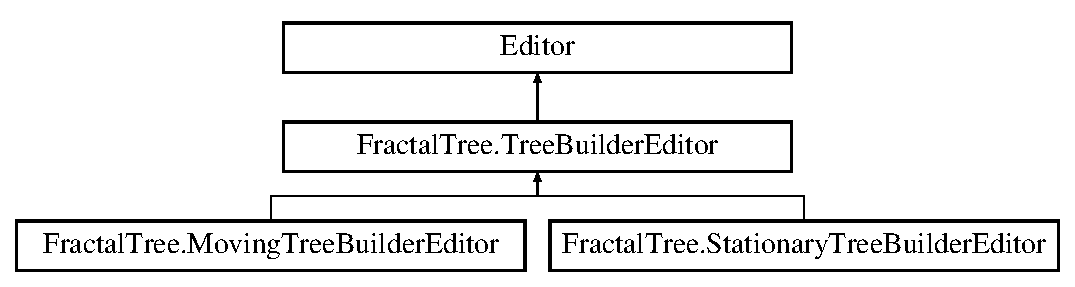
\includegraphics[height=3.000000cm]{class_fractal_tree_1_1_tree_builder_editor}
\end{center}
\end{figure}
\subsection*{Protected Member Functions}
\begin{DoxyCompactItemize}
\item 
\mbox{\Hypertarget{class_fractal_tree_1_1_tree_builder_editor_a5d41488772ecce6513f4fb335ae1e584}\label{class_fractal_tree_1_1_tree_builder_editor_a5d41488772ecce6513f4fb335ae1e584}} 
void {\bfseries Draw\+Editor} ()
\end{DoxyCompactItemize}


\subsection{Detailed Description}
Custom editor for tree builder class. Hides variables not in use based on Tree\+Type. 



The documentation for this class was generated from the following file\+:\begin{DoxyCompactItemize}
\item 
F\+T/\+Scripts/\+Editor/Tree\+Builder\+Editor.\+cs\end{DoxyCompactItemize}

\hypertarget{class_fractal_tree_1_1_demo_1_1_trees_to_demo}{}\section{Fractal\+Tree.\+Demo.\+Trees\+To\+Demo Class Reference}
\label{class_fractal_tree_1_1_demo_1_1_trees_to_demo}\index{Fractal\+Tree.\+Demo.\+Trees\+To\+Demo@{Fractal\+Tree.\+Demo.\+Trees\+To\+Demo}}


Trees to demo. Stationary and Moving tree builder pairs.  


\subsection*{Public Member Functions}
\begin{DoxyCompactItemize}
\item 
void \hyperlink{class_fractal_tree_1_1_demo_1_1_trees_to_demo_a619aeb9379dfe3fdd85c881d7d1703e3}{Build\+Stationary} ()
\begin{DoxyCompactList}\small\item\em Builds the stationary tree and then disables game object. \end{DoxyCompactList}\item 
void \hyperlink{class_fractal_tree_1_1_demo_1_1_trees_to_demo_afad82e3ecd0f549ad278cd912050491d}{Build\+Moving} ()
\begin{DoxyCompactList}\small\item\em Builds the moving tree and then disables game object. \end{DoxyCompactList}\item 
void \hyperlink{class_fractal_tree_1_1_demo_1_1_trees_to_demo_abe09f9d37ec9b04f06abd2bef66aed72}{Show} (bool show\+Stationary)
\begin{DoxyCompactList}\small\item\em Enables either the stationary or moving tree. \end{DoxyCompactList}\item 
void \hyperlink{class_fractal_tree_1_1_demo_1_1_trees_to_demo_a9d6e9bb23591884f3bf2a5957095390e}{Hide} ()
\begin{DoxyCompactList}\small\item\em Disables both trees. \end{DoxyCompactList}\end{DoxyCompactItemize}
\subsection*{Public Attributes}
\begin{DoxyCompactItemize}
\item 
\mbox{\Hypertarget{class_fractal_tree_1_1_demo_1_1_trees_to_demo_a9c065899e43c7cc2a9d84601e39dc4a5}\label{class_fractal_tree_1_1_demo_1_1_trees_to_demo_a9c065899e43c7cc2a9d84601e39dc4a5}} 
bool {\bfseries preload}
\item 
\mbox{\Hypertarget{class_fractal_tree_1_1_demo_1_1_trees_to_demo_a6e9e96dbbfe2710d3c0faf37ccd3ea61}\label{class_fractal_tree_1_1_demo_1_1_trees_to_demo_a6e9e96dbbfe2710d3c0faf37ccd3ea61}} 
bool {\bfseries built}
\item 
\hyperlink{class_fractal_tree_1_1_tree_builder}{Tree\+Builder} \hyperlink{class_fractal_tree_1_1_demo_1_1_trees_to_demo_aa5d13795814c54312725bbe500a0c05b}{stationary\+Tree}
\begin{DoxyCompactList}\small\item\em The stationary tree. \end{DoxyCompactList}\item 
\hyperlink{class_fractal_tree_1_1_tree_builder}{Tree\+Builder} \hyperlink{class_fractal_tree_1_1_demo_1_1_trees_to_demo_a8ebc7052928d860fd758a5ecfbff5710}{moving\+Tree}
\begin{DoxyCompactList}\small\item\em The moving tree. \end{DoxyCompactList}\end{DoxyCompactItemize}
\subsection*{Properties}
\begin{DoxyCompactItemize}
\item 
\hyperlink{class_fractal_tree_1_1_tree_builder}{Tree\+Builder} \hyperlink{class_fractal_tree_1_1_demo_1_1_trees_to_demo_a4c255b3c34a65405fd1c69a81bb9a0a0}{active}\hspace{0.3cm}{\ttfamily  \mbox{[}get\mbox{]}}
\begin{DoxyCompactList}\small\item\em Gets the active tree builder. \end{DoxyCompactList}\end{DoxyCompactItemize}


\subsection{Detailed Description}
Trees to demo. Stationary and Moving tree builder pairs. 



\subsection{Member Function Documentation}
\mbox{\Hypertarget{class_fractal_tree_1_1_demo_1_1_trees_to_demo_afad82e3ecd0f549ad278cd912050491d}\label{class_fractal_tree_1_1_demo_1_1_trees_to_demo_afad82e3ecd0f549ad278cd912050491d}} 
\index{Fractal\+Tree\+::\+Demo\+::\+Trees\+To\+Demo@{Fractal\+Tree\+::\+Demo\+::\+Trees\+To\+Demo}!Build\+Moving@{Build\+Moving}}
\index{Build\+Moving@{Build\+Moving}!Fractal\+Tree\+::\+Demo\+::\+Trees\+To\+Demo@{Fractal\+Tree\+::\+Demo\+::\+Trees\+To\+Demo}}
\subsubsection{\texorpdfstring{Build\+Moving()}{BuildMoving()}}
{\footnotesize\ttfamily void Fractal\+Tree.\+Demo.\+Trees\+To\+Demo.\+Build\+Moving (\begin{DoxyParamCaption}{ }\end{DoxyParamCaption})}



Builds the moving tree and then disables game object. 

\mbox{\Hypertarget{class_fractal_tree_1_1_demo_1_1_trees_to_demo_a619aeb9379dfe3fdd85c881d7d1703e3}\label{class_fractal_tree_1_1_demo_1_1_trees_to_demo_a619aeb9379dfe3fdd85c881d7d1703e3}} 
\index{Fractal\+Tree\+::\+Demo\+::\+Trees\+To\+Demo@{Fractal\+Tree\+::\+Demo\+::\+Trees\+To\+Demo}!Build\+Stationary@{Build\+Stationary}}
\index{Build\+Stationary@{Build\+Stationary}!Fractal\+Tree\+::\+Demo\+::\+Trees\+To\+Demo@{Fractal\+Tree\+::\+Demo\+::\+Trees\+To\+Demo}}
\subsubsection{\texorpdfstring{Build\+Stationary()}{BuildStationary()}}
{\footnotesize\ttfamily void Fractal\+Tree.\+Demo.\+Trees\+To\+Demo.\+Build\+Stationary (\begin{DoxyParamCaption}{ }\end{DoxyParamCaption})}



Builds the stationary tree and then disables game object. 

\mbox{\Hypertarget{class_fractal_tree_1_1_demo_1_1_trees_to_demo_a9d6e9bb23591884f3bf2a5957095390e}\label{class_fractal_tree_1_1_demo_1_1_trees_to_demo_a9d6e9bb23591884f3bf2a5957095390e}} 
\index{Fractal\+Tree\+::\+Demo\+::\+Trees\+To\+Demo@{Fractal\+Tree\+::\+Demo\+::\+Trees\+To\+Demo}!Hide@{Hide}}
\index{Hide@{Hide}!Fractal\+Tree\+::\+Demo\+::\+Trees\+To\+Demo@{Fractal\+Tree\+::\+Demo\+::\+Trees\+To\+Demo}}
\subsubsection{\texorpdfstring{Hide()}{Hide()}}
{\footnotesize\ttfamily void Fractal\+Tree.\+Demo.\+Trees\+To\+Demo.\+Hide (\begin{DoxyParamCaption}{ }\end{DoxyParamCaption})}



Disables both trees. 

\mbox{\Hypertarget{class_fractal_tree_1_1_demo_1_1_trees_to_demo_abe09f9d37ec9b04f06abd2bef66aed72}\label{class_fractal_tree_1_1_demo_1_1_trees_to_demo_abe09f9d37ec9b04f06abd2bef66aed72}} 
\index{Fractal\+Tree\+::\+Demo\+::\+Trees\+To\+Demo@{Fractal\+Tree\+::\+Demo\+::\+Trees\+To\+Demo}!Show@{Show}}
\index{Show@{Show}!Fractal\+Tree\+::\+Demo\+::\+Trees\+To\+Demo@{Fractal\+Tree\+::\+Demo\+::\+Trees\+To\+Demo}}
\subsubsection{\texorpdfstring{Show()}{Show()}}
{\footnotesize\ttfamily void Fractal\+Tree.\+Demo.\+Trees\+To\+Demo.\+Show (\begin{DoxyParamCaption}\item[{bool}]{show\+Stationary }\end{DoxyParamCaption})}



Enables either the stationary or moving tree. 


\begin{DoxyParams}{Parameters}
{\em show\+Stationary} & If set to {\ttfamily true} show stationary else show moving tree.\\
\hline
\end{DoxyParams}


\subsection{Member Data Documentation}
\mbox{\Hypertarget{class_fractal_tree_1_1_demo_1_1_trees_to_demo_a8ebc7052928d860fd758a5ecfbff5710}\label{class_fractal_tree_1_1_demo_1_1_trees_to_demo_a8ebc7052928d860fd758a5ecfbff5710}} 
\index{Fractal\+Tree\+::\+Demo\+::\+Trees\+To\+Demo@{Fractal\+Tree\+::\+Demo\+::\+Trees\+To\+Demo}!moving\+Tree@{moving\+Tree}}
\index{moving\+Tree@{moving\+Tree}!Fractal\+Tree\+::\+Demo\+::\+Trees\+To\+Demo@{Fractal\+Tree\+::\+Demo\+::\+Trees\+To\+Demo}}
\subsubsection{\texorpdfstring{moving\+Tree}{movingTree}}
{\footnotesize\ttfamily \hyperlink{class_fractal_tree_1_1_tree_builder}{Tree\+Builder} Fractal\+Tree.\+Demo.\+Trees\+To\+Demo.\+moving\+Tree}



The moving tree. 

\mbox{\Hypertarget{class_fractal_tree_1_1_demo_1_1_trees_to_demo_aa5d13795814c54312725bbe500a0c05b}\label{class_fractal_tree_1_1_demo_1_1_trees_to_demo_aa5d13795814c54312725bbe500a0c05b}} 
\index{Fractal\+Tree\+::\+Demo\+::\+Trees\+To\+Demo@{Fractal\+Tree\+::\+Demo\+::\+Trees\+To\+Demo}!stationary\+Tree@{stationary\+Tree}}
\index{stationary\+Tree@{stationary\+Tree}!Fractal\+Tree\+::\+Demo\+::\+Trees\+To\+Demo@{Fractal\+Tree\+::\+Demo\+::\+Trees\+To\+Demo}}
\subsubsection{\texorpdfstring{stationary\+Tree}{stationaryTree}}
{\footnotesize\ttfamily \hyperlink{class_fractal_tree_1_1_tree_builder}{Tree\+Builder} Fractal\+Tree.\+Demo.\+Trees\+To\+Demo.\+stationary\+Tree}



The stationary tree. 



\subsection{Property Documentation}
\mbox{\Hypertarget{class_fractal_tree_1_1_demo_1_1_trees_to_demo_a4c255b3c34a65405fd1c69a81bb9a0a0}\label{class_fractal_tree_1_1_demo_1_1_trees_to_demo_a4c255b3c34a65405fd1c69a81bb9a0a0}} 
\index{Fractal\+Tree\+::\+Demo\+::\+Trees\+To\+Demo@{Fractal\+Tree\+::\+Demo\+::\+Trees\+To\+Demo}!active@{active}}
\index{active@{active}!Fractal\+Tree\+::\+Demo\+::\+Trees\+To\+Demo@{Fractal\+Tree\+::\+Demo\+::\+Trees\+To\+Demo}}
\subsubsection{\texorpdfstring{active}{active}}
{\footnotesize\ttfamily \hyperlink{class_fractal_tree_1_1_tree_builder}{Tree\+Builder} Fractal\+Tree.\+Demo.\+Trees\+To\+Demo.\+active\hspace{0.3cm}{\ttfamily [get]}}



Gets the active tree builder. 

The active.

The documentation for this class was generated from the following file\+:\begin{DoxyCompactItemize}
\item 
F\+T/\+Scripts/\+Demo/Demo\+Tree\+Creator.\+cs\end{DoxyCompactItemize}

%--- End generated contents ---

% Index
\backmatter
\newpage
\phantomsection
\clearemptydoublepage
\addcontentsline{toc}{chapter}{Index}
\printindex

\end{document}
